


% Header, overrides base

    % Make sure that the sphinx doc style knows who it inherits from.
    \def\sphinxdocclass{article}

    % Declare the document class
    \documentclass[letterpaper,10pt,english]{/Users/qcaudron/anaconda/lib/python2.7/site-packages/Sphinx-1.2b1-py2.7.egg/sphinx/texinputs/sphinxhowto}

    % Imports
    \usepackage[utf8]{inputenc}
    \DeclareUnicodeCharacter{00A0}{\\nobreakspace}
    \usepackage[T1]{fontenc}
    \usepackage{babel}
    \usepackage{times}
    \usepackage{import}
    \usepackage[Bjarne]{/Users/qcaudron/anaconda/lib/python2.7/site-packages/Sphinx-1.2b1-py2.7.egg/sphinx/texinputs/fncychap}
    \usepackage{longtable}
    \usepackage{/Users/qcaudron/anaconda/lib/python2.7/site-packages/Sphinx-1.2b1-py2.7.egg/sphinx/texinputs/sphinx}
    \usepackage{multirow}

    \usepackage{amsmath}
    \usepackage{amssymb}
    \usepackage{ucs}
    \usepackage{enumerate}

    % Used to make the Input/Output rules follow around the contents.
    \usepackage{needspace}

    % Pygments requirements
    \usepackage{fancyvrb}
    \usepackage{color}
    % ansi colors additions
    \definecolor{darkgreen}{rgb}{.12,.54,.11}
    \definecolor{lightgray}{gray}{.95}
    \definecolor{brown}{rgb}{0.54,0.27,0.07}
    \definecolor{purple}{rgb}{0.5,0.0,0.5}
    \definecolor{darkgray}{gray}{0.25}
    \definecolor{lightred}{rgb}{1.0,0.39,0.28}
    \definecolor{lightgreen}{rgb}{0.48,0.99,0.0}
    \definecolor{lightblue}{rgb}{0.53,0.81,0.92}
    \definecolor{lightpurple}{rgb}{0.87,0.63,0.87}
    \definecolor{lightcyan}{rgb}{0.5,1.0,0.83}

    % Needed to box output/input
    \usepackage{tikz}
        \usetikzlibrary{calc,arrows,shadows}
    \usepackage[framemethod=tikz]{mdframed}

    \usepackage{alltt}

    % Used to load and display graphics
    \usepackage{graphicx}
    \graphicspath{ {figs/} }
    \usepackage[Export]{adjustbox} % To resize

    % used so that images for notebooks which have spaces in the name can still be included
    \usepackage{grffile}


    % For formatting output while also word wrapping.
    \usepackage{listings}
    \lstset{breaklines=true}
    \lstset{basicstyle=\small\ttfamily}
    \def\smaller{\fontsize{9.5pt}{9.5pt}\selectfont}

    %Pygments definitions
    
\makeatletter
\def\PY@reset{\let\PY@it=\relax \let\PY@bf=\relax%
    \let\PY@ul=\relax \let\PY@tc=\relax%
    \let\PY@bc=\relax \let\PY@ff=\relax}
\def\PY@tok#1{\csname PY@tok@#1\endcsname}
\def\PY@toks#1+{\ifx\relax#1\empty\else%
    \PY@tok{#1}\expandafter\PY@toks\fi}
\def\PY@do#1{\PY@bc{\PY@tc{\PY@ul{%
    \PY@it{\PY@bf{\PY@ff{#1}}}}}}}
\def\PY#1#2{\PY@reset\PY@toks#1+\relax+\PY@do{#2}}

\expandafter\def\csname PY@tok@gd\endcsname{\def\PY@tc##1{\textcolor[rgb]{0.63,0.00,0.00}{##1}}}
\expandafter\def\csname PY@tok@gu\endcsname{\let\PY@bf=\textbf\def\PY@tc##1{\textcolor[rgb]{0.50,0.00,0.50}{##1}}}
\expandafter\def\csname PY@tok@gt\endcsname{\def\PY@tc##1{\textcolor[rgb]{0.00,0.27,0.87}{##1}}}
\expandafter\def\csname PY@tok@gs\endcsname{\let\PY@bf=\textbf}
\expandafter\def\csname PY@tok@gr\endcsname{\def\PY@tc##1{\textcolor[rgb]{1.00,0.00,0.00}{##1}}}
\expandafter\def\csname PY@tok@cm\endcsname{\let\PY@it=\textit\def\PY@tc##1{\textcolor[rgb]{0.25,0.50,0.50}{##1}}}
\expandafter\def\csname PY@tok@vg\endcsname{\def\PY@tc##1{\textcolor[rgb]{0.10,0.09,0.49}{##1}}}
\expandafter\def\csname PY@tok@m\endcsname{\def\PY@tc##1{\textcolor[rgb]{0.40,0.40,0.40}{##1}}}
\expandafter\def\csname PY@tok@mh\endcsname{\def\PY@tc##1{\textcolor[rgb]{0.40,0.40,0.40}{##1}}}
\expandafter\def\csname PY@tok@go\endcsname{\def\PY@tc##1{\textcolor[rgb]{0.53,0.53,0.53}{##1}}}
\expandafter\def\csname PY@tok@ge\endcsname{\let\PY@it=\textit}
\expandafter\def\csname PY@tok@vc\endcsname{\def\PY@tc##1{\textcolor[rgb]{0.10,0.09,0.49}{##1}}}
\expandafter\def\csname PY@tok@il\endcsname{\def\PY@tc##1{\textcolor[rgb]{0.40,0.40,0.40}{##1}}}
\expandafter\def\csname PY@tok@cs\endcsname{\let\PY@it=\textit\def\PY@tc##1{\textcolor[rgb]{0.25,0.50,0.50}{##1}}}
\expandafter\def\csname PY@tok@cp\endcsname{\def\PY@tc##1{\textcolor[rgb]{0.74,0.48,0.00}{##1}}}
\expandafter\def\csname PY@tok@gi\endcsname{\def\PY@tc##1{\textcolor[rgb]{0.00,0.63,0.00}{##1}}}
\expandafter\def\csname PY@tok@gh\endcsname{\let\PY@bf=\textbf\def\PY@tc##1{\textcolor[rgb]{0.00,0.00,0.50}{##1}}}
\expandafter\def\csname PY@tok@ni\endcsname{\let\PY@bf=\textbf\def\PY@tc##1{\textcolor[rgb]{0.60,0.60,0.60}{##1}}}
\expandafter\def\csname PY@tok@nl\endcsname{\def\PY@tc##1{\textcolor[rgb]{0.63,0.63,0.00}{##1}}}
\expandafter\def\csname PY@tok@nn\endcsname{\let\PY@bf=\textbf\def\PY@tc##1{\textcolor[rgb]{0.00,0.00,1.00}{##1}}}
\expandafter\def\csname PY@tok@no\endcsname{\def\PY@tc##1{\textcolor[rgb]{0.53,0.00,0.00}{##1}}}
\expandafter\def\csname PY@tok@na\endcsname{\def\PY@tc##1{\textcolor[rgb]{0.49,0.56,0.16}{##1}}}
\expandafter\def\csname PY@tok@nb\endcsname{\def\PY@tc##1{\textcolor[rgb]{0.00,0.50,0.00}{##1}}}
\expandafter\def\csname PY@tok@nc\endcsname{\let\PY@bf=\textbf\def\PY@tc##1{\textcolor[rgb]{0.00,0.00,1.00}{##1}}}
\expandafter\def\csname PY@tok@nd\endcsname{\def\PY@tc##1{\textcolor[rgb]{0.67,0.13,1.00}{##1}}}
\expandafter\def\csname PY@tok@ne\endcsname{\let\PY@bf=\textbf\def\PY@tc##1{\textcolor[rgb]{0.82,0.25,0.23}{##1}}}
\expandafter\def\csname PY@tok@nf\endcsname{\def\PY@tc##1{\textcolor[rgb]{0.00,0.00,1.00}{##1}}}
\expandafter\def\csname PY@tok@si\endcsname{\let\PY@bf=\textbf\def\PY@tc##1{\textcolor[rgb]{0.73,0.40,0.53}{##1}}}
\expandafter\def\csname PY@tok@s2\endcsname{\def\PY@tc##1{\textcolor[rgb]{0.73,0.13,0.13}{##1}}}
\expandafter\def\csname PY@tok@vi\endcsname{\def\PY@tc##1{\textcolor[rgb]{0.10,0.09,0.49}{##1}}}
\expandafter\def\csname PY@tok@nt\endcsname{\let\PY@bf=\textbf\def\PY@tc##1{\textcolor[rgb]{0.00,0.50,0.00}{##1}}}
\expandafter\def\csname PY@tok@nv\endcsname{\def\PY@tc##1{\textcolor[rgb]{0.10,0.09,0.49}{##1}}}
\expandafter\def\csname PY@tok@s1\endcsname{\def\PY@tc##1{\textcolor[rgb]{0.73,0.13,0.13}{##1}}}
\expandafter\def\csname PY@tok@sh\endcsname{\def\PY@tc##1{\textcolor[rgb]{0.73,0.13,0.13}{##1}}}
\expandafter\def\csname PY@tok@sc\endcsname{\def\PY@tc##1{\textcolor[rgb]{0.73,0.13,0.13}{##1}}}
\expandafter\def\csname PY@tok@sx\endcsname{\def\PY@tc##1{\textcolor[rgb]{0.00,0.50,0.00}{##1}}}
\expandafter\def\csname PY@tok@bp\endcsname{\def\PY@tc##1{\textcolor[rgb]{0.00,0.50,0.00}{##1}}}
\expandafter\def\csname PY@tok@c1\endcsname{\let\PY@it=\textit\def\PY@tc##1{\textcolor[rgb]{0.25,0.50,0.50}{##1}}}
\expandafter\def\csname PY@tok@kc\endcsname{\let\PY@bf=\textbf\def\PY@tc##1{\textcolor[rgb]{0.00,0.50,0.00}{##1}}}
\expandafter\def\csname PY@tok@c\endcsname{\let\PY@it=\textit\def\PY@tc##1{\textcolor[rgb]{0.25,0.50,0.50}{##1}}}
\expandafter\def\csname PY@tok@mf\endcsname{\def\PY@tc##1{\textcolor[rgb]{0.40,0.40,0.40}{##1}}}
\expandafter\def\csname PY@tok@err\endcsname{\def\PY@bc##1{\setlength{\fboxsep}{0pt}\fcolorbox[rgb]{1.00,0.00,0.00}{1,1,1}{\strut ##1}}}
\expandafter\def\csname PY@tok@kd\endcsname{\let\PY@bf=\textbf\def\PY@tc##1{\textcolor[rgb]{0.00,0.50,0.00}{##1}}}
\expandafter\def\csname PY@tok@ss\endcsname{\def\PY@tc##1{\textcolor[rgb]{0.10,0.09,0.49}{##1}}}
\expandafter\def\csname PY@tok@sr\endcsname{\def\PY@tc##1{\textcolor[rgb]{0.73,0.40,0.53}{##1}}}
\expandafter\def\csname PY@tok@mo\endcsname{\def\PY@tc##1{\textcolor[rgb]{0.40,0.40,0.40}{##1}}}
\expandafter\def\csname PY@tok@kn\endcsname{\let\PY@bf=\textbf\def\PY@tc##1{\textcolor[rgb]{0.00,0.50,0.00}{##1}}}
\expandafter\def\csname PY@tok@mi\endcsname{\def\PY@tc##1{\textcolor[rgb]{0.40,0.40,0.40}{##1}}}
\expandafter\def\csname PY@tok@gp\endcsname{\let\PY@bf=\textbf\def\PY@tc##1{\textcolor[rgb]{0.00,0.00,0.50}{##1}}}
\expandafter\def\csname PY@tok@o\endcsname{\def\PY@tc##1{\textcolor[rgb]{0.40,0.40,0.40}{##1}}}
\expandafter\def\csname PY@tok@kr\endcsname{\let\PY@bf=\textbf\def\PY@tc##1{\textcolor[rgb]{0.00,0.50,0.00}{##1}}}
\expandafter\def\csname PY@tok@s\endcsname{\def\PY@tc##1{\textcolor[rgb]{0.73,0.13,0.13}{##1}}}
\expandafter\def\csname PY@tok@kp\endcsname{\def\PY@tc##1{\textcolor[rgb]{0.00,0.50,0.00}{##1}}}
\expandafter\def\csname PY@tok@w\endcsname{\def\PY@tc##1{\textcolor[rgb]{0.73,0.73,0.73}{##1}}}
\expandafter\def\csname PY@tok@kt\endcsname{\def\PY@tc##1{\textcolor[rgb]{0.69,0.00,0.25}{##1}}}
\expandafter\def\csname PY@tok@ow\endcsname{\let\PY@bf=\textbf\def\PY@tc##1{\textcolor[rgb]{0.67,0.13,1.00}{##1}}}
\expandafter\def\csname PY@tok@sb\endcsname{\def\PY@tc##1{\textcolor[rgb]{0.73,0.13,0.13}{##1}}}
\expandafter\def\csname PY@tok@k\endcsname{\let\PY@bf=\textbf\def\PY@tc##1{\textcolor[rgb]{0.00,0.50,0.00}{##1}}}
\expandafter\def\csname PY@tok@se\endcsname{\let\PY@bf=\textbf\def\PY@tc##1{\textcolor[rgb]{0.73,0.40,0.13}{##1}}}
\expandafter\def\csname PY@tok@sd\endcsname{\let\PY@it=\textit\def\PY@tc##1{\textcolor[rgb]{0.73,0.13,0.13}{##1}}}

\def\PYZbs{\char`\\}
\def\PYZus{\char`\_}
\def\PYZob{\char`\{}
\def\PYZcb{\char`\}}
\def\PYZca{\char`\^}
\def\PYZam{\char`\&}
\def\PYZlt{\char`\<}
\def\PYZgt{\char`\>}
\def\PYZsh{\char`\#}
\def\PYZpc{\char`\%}
\def\PYZdl{\char`\$}
\def\PYZhy{\char`\-}
\def\PYZsq{\char`\'}
\def\PYZdq{\char`\"}
\def\PYZti{\char`\~}
% for compatibility with earlier versions
\def\PYZat{@}
\def\PYZlb{[}
\def\PYZrb{]}
\makeatother


    %Set pygments styles if needed...
    
        \definecolor{nbframe-border}{rgb}{0.867,0.867,0.867}
        \definecolor{nbframe-bg}{rgb}{0.969,0.969,0.969}
        \definecolor{nbframe-in-prompt}{rgb}{0.0,0.0,0.502}
        \definecolor{nbframe-out-prompt}{rgb}{0.545,0.0,0.0}

        \newenvironment{ColorVerbatim}
        {\begin{mdframed}[%
            roundcorner=1.0pt, %
            backgroundcolor=nbframe-bg, %
            userdefinedwidth=1\linewidth, %
            leftmargin=0.1\linewidth, %
            innerleftmargin=0pt, %
            innerrightmargin=0pt, %
            linecolor=nbframe-border, %
            linewidth=1pt, %
            usetwoside=false, %
            everyline=true, %
            innerlinewidth=3pt, %
            innerlinecolor=nbframe-bg, %
            middlelinewidth=1pt, %
            middlelinecolor=nbframe-bg, %
            outerlinewidth=0.5pt, %
            outerlinecolor=nbframe-border, %
            needspace=0pt
        ]}
        {\end{mdframed}}
        
        \newenvironment{InvisibleVerbatim}
        {\begin{mdframed}[leftmargin=0.1\linewidth,innerleftmargin=3pt,innerrightmargin=3pt, userdefinedwidth=1\linewidth, linewidth=0pt, linecolor=white, usetwoside=false]}
        {\end{mdframed}}

        \renewenvironment{Verbatim}[1][\unskip]
        {\begin{alltt}\smaller}
        {\end{alltt}}
    

    % Help prevent overflowing lines due to urls and other hard-to-break 
    % entities.  This doesn't catch everything...
    \sloppy

    % Document level variables
    \title{notebook}
    \date{March 12, 2014}
    \release{}
    \author{Unknown Author}
    \renewcommand{\releasename}{}

    % TODO: Add option for the user to specify a logo for his/her export.
    \newcommand{\sphinxlogo}{}

    % Make the index page of the document.
    \makeindex

    % Import sphinx document type specifics.
     


% Body

    % Start of the document
    \begin{document}

        
            \maketitle
        

        


        
        \part{Measles in Small Populations}Based on \emph{Finkenstadt and Grenfell (2002), Applied Statistics}, the
paper introducing the TSIR model. The model relates $S_t$, the number of
susceptibles at time $t$, to the number of infected cases $I_t$ at time
$t$ :

\[
I_{t+1} = r_t \, S_t \, I_t^\alpha \, \varepsilon_t,
\] \[
S_{t+1} = B_{t-d} + S_t - I_t + u_t
\]

where $r_t$ is a positive seasonal contact rate parameter; $B_t$ are the
births during timestep $t$; $\varepsilon_t$ and $u_t$ are Gaussian
noises with $\mathrm{E}[\varepsilon_t] = 1$ and $\mathrm{E}[u_t] = 0$;
and $\alpha \in (0, 1]$ is a homogeneity parameter, with $\alpha = 1$
equivalent to mass action dynamics.

    % Make sure that atleast 4 lines are below the HR
    \needspace{4\baselineskip}

    
        \vspace{6pt}
        \makebox[0.1\linewidth]{\smaller\hfill\tt\color{nbframe-in-prompt}In\hspace{4pt}{[}3{]}:\hspace{4pt}}\\*
        \vspace{-2.65\baselineskip}
        \begin{ColorVerbatim}
            \vspace{-0.7\baselineskip}
            \begin{Verbatim}[commandchars=\\\{\}]
\PY{c}{\PYZsh{}\PYZsh{} IMPORTS}

\PY{c}{\PYZsh{} Numerical packages and methods}
\PY{k+kn}{import} \PY{n+nn}{numpy} \PY{k+kn}{as} \PY{n+nn}{np}
\PY{k+kn}{from} \PY{n+nn}{sklearn} \PY{k+kn}{import} \PY{n}{linear\PYZus{}model}
\PY{k+kn}{from} \PY{n+nn}{scipy.optimize} \PY{k+kn}{import} \PY{n}{curve\PYZus{}fit}
\PY{k+kn}{import} \PY{n+nn}{scipy.stats} \PY{k+kn}{as} \PY{n+nn}{st}
\PY{k+kn}{import} \PY{n+nn}{scipy.interpolate} \PY{k+kn}{as} \PY{n+nn}{interp}

\PY{c}{\PYZsh{} Monte Carlo and Nonlinear Fitting}
\PY{k+kn}{import} \PY{n+nn}{pymc}
\PY{k+kn}{import} \PY{n+nn}{lmfit}

\PY{c}{\PYZsh{} Plotting}
\PY{k+kn}{import} \PY{n+nn}{matplotlib}
\PY{k+kn}{from} \PY{n+nn}{prettyplotlib} \PY{k+kn}{import} \PY{n}{plt}
\PY{k+kn}{import} \PY{n+nn}{brewer2mpl}
\PY{n}{matplotlib}\PY{o}{.}\PY{n}{rcParams}\PY{p}{[}\PY{l+s}{\PYZsq{}}\PY{l+s}{savefig.dpi}\PY{l+s}{\PYZsq{}}\PY{p}{]} \PY{o}{=} \PY{l+m+mf}{1.8} \PY{o}{*} \PY{n}{matplotlib}\PY{o}{.}\PY{n}{rcParams}\PY{p}{[}\PY{l+s}{\PYZsq{}}\PY{l+s}{savefig.dpi}\PY{l+s}{\PYZsq{}}\PY{p}{]}
\PY{n}{figsize}\PY{p}{(}\PY{l+m+mi}{14}\PY{p}{,} \PY{l+m+mi}{8}\PY{p}{)}
\PY{n}{colours} \PY{o}{=} \PY{n}{brewer2mpl}\PY{o}{.}\PY{n}{get\PYZus{}map}\PY{p}{(}\PY{l+s}{\PYZsq{}}\PY{l+s}{Set2}\PY{l+s}{\PYZsq{}}\PY{p}{,} \PY{l+s}{\PYZsq{}}\PY{l+s}{qualitative}\PY{l+s}{\PYZsq{}}\PY{p}{,} \PY{l+m+mi}{8}\PY{p}{)}\PY{o}{.}\PY{n}{mpl\PYZus{}colors}
\PY{c}{\PYZsh{}import seaborn}

\PY{c}{\PYZsh{} Other}
\PY{k+kn}{import} \PY{n+nn}{itertools}
\end{Verbatim}

            
                \vspace{-0.2\baselineskip}
            
        \end{ColorVerbatim}
    
\textbf{Data}

We have several import options. Of the four variables, \texttt{LONDON},
\texttt{ICELAND}, \texttt{FAROE}, and \texttt{BORNHOLM}, only one is
allowed to be 1. This selects the source of data to import and analyse.
If all are 0, we instead simulate an SIR model at equilibrium with major
biennial epidemics and minor epidemics in between - that is, measles in
a large, well-mixed population. If more than one of these variables are
1, we import the first non-zero.

    % Make sure that atleast 4 lines are below the HR
    \needspace{4\baselineskip}

    
        \vspace{6pt}
        \makebox[0.1\linewidth]{\smaller\hfill\tt\color{nbframe-in-prompt}In\hspace{4pt}{[}11{]}:\hspace{4pt}}\\*
        \vspace{-2.65\baselineskip}
        \begin{ColorVerbatim}
            \vspace{-0.7\baselineskip}
            \begin{Verbatim}[commandchars=\\\{\}]
\PY{c}{\PYZsh{} Import what ?}
\PY{n}{LONDON} \PY{o}{=} \PY{l+m+mi}{0}
\PY{n}{ICELAND} \PY{o}{=} \PY{l+m+mi}{0}
\PY{n}{FAROE} \PY{o}{=} \PY{l+m+mi}{1}
\PY{n}{BORNHOLM} \PY{o}{=} \PY{l+m+mi}{0}
\end{Verbatim}

            
                \vspace{-0.2\baselineskip}
            
        \end{ColorVerbatim}
    
\textbf{Model Parameters}

The \texttt{periodicity} of the time series imposes an infectious
period. A periodicity of 24 implies the infectious period is 1/24 years,
or 15.2 days. 24 is chosen to optimise the result of the interpolation
of monthly-sampled time series, as we have for Iceland, the Faroe
Islands, and Bornholm. London must be dealt with differently, due to its
biweekly-sampled time series. Its periodicity is thus 26.

The \texttt{delay} is an estimate of the number of periods of infection
during which newly-born susceptibles are immune to infection due to
maternal antibodies. Here, we assume four months, or eight periods of
about fifteen days ( fourteen for London ).

The model's \texttt{sensitivity} determines how many cases of measles
are required for a given time point to be considered as being part of an
epidemic.

Finally, \texttt{penalty} is used as a weighting parameter to avoid
overfitting during susceptible reconstruction. This step is done using
an arbitrary polynomial; \texttt{penalty} ensures that higher degree
polynomials are not selected due to overfitting.

\textbf{Interpolation}

The incidence data for London is biweekly, and does not need to be
interpolated. Incidence data for Iceland, the Faroe Islands, and
Bornholm, are all monthly, and need to be interpolated. To avoid
artifacts due to shifting timepoints in the series, we can either use
splines, or use a number of timepoints that is a multiple of the current
sampling. We opt for the latter here, as splines introduce a large
number of oscillations in the derivatives, due to their nature as a
piecewise cubic function.

Birth rates are interpolated in the same manner.

    % Make sure that atleast 4 lines are below the HR
    \needspace{4\baselineskip}

    
        \vspace{6pt}
        \makebox[0.1\linewidth]{\smaller\hfill\tt\color{nbframe-in-prompt}In\hspace{4pt}{[}14{]}:\hspace{4pt}}\\*
        \vspace{-2.65\baselineskip}
        \begin{ColorVerbatim}
            \vspace{-0.7\baselineskip}
            \begin{Verbatim}[commandchars=\\\{\}]
\PY{c}{\PYZsh{} Model parameters}
\PY{n}{periodicity} \PY{o}{=} \PY{l+m+mi}{24} \PY{k}{if} \PY{o+ow}{not} \PY{n}{LONDON} \PY{k}{else} \PY{l+m+mi}{26}
\PY{n}{delay} \PY{o}{=} \PY{l+m+mi}{8}
\PY{n}{sensitivity} \PY{o}{=} \PY{l+m+mi}{2}
\PY{n}{penalty} \PY{o}{=} \PY{l+m+mf}{5e\PYZhy{}4}

\PY{c}{\PYZsh{}if FAROE :}
\PY{c}{\PYZsh{}    sensitivity = 25}
\PY{c}{\PYZsh{}elif ICELAND :}
\PY{c}{\PYZsh{}    sensitivity = 15}



\PY{c}{\PYZsh{} Import data}
\PY{k}{if} \PY{o+ow}{not} \PY{p}{(}\PY{n}{LONDON} \PY{o+ow}{or} \PY{n}{ICELAND} \PY{o+ow}{or} \PY{n}{FAROE} \PY{o+ow}{or} \PY{n}{BORNHOLM}\PY{p}{)} \PY{p}{:} \PY{c}{\PYZsh{} then simulate SIR dynamics}
    
    \PY{c}{\PYZsh{} Timestep, maximum time ( in periods ), and model\PYZhy{}time array}
    \PY{n}{dt} \PY{o}{=} \PY{o}{.}\PY{l+m+mo}{05}
    \PY{n}{tmax} \PY{o}{=} \PY{l+m+mi}{2000}
    \PY{n}{mt} \PY{o}{=} \PY{n}{np}\PY{o}{.}\PY{n}{arange}\PY{p}{(}\PY{l+m+mi}{0}\PY{p}{,} \PY{n}{tmax}\PY{p}{,} \PY{n}{dt}\PY{p}{)}
    
    
    \PY{c}{\PYZsh{} Population Parameters :}
    \PY{n}{N} \PY{o}{=} \PY{l+m+mf}{3e6} \PY{c}{\PYZsh{} total population}
    \PY{n}{mu} \PY{o}{=} \PY{n}{np}\PY{o}{.}\PY{n}{ones}\PY{p}{(}\PY{n+nb}{int}\PY{p}{(}\PY{n}{tmax}\PY{o}{/}\PY{n}{dt}\PY{p}{)}\PY{p}{,}\PY{p}{)} \PY{o}{*} \PY{l+m+mf}{1.}\PY{o}{/}\PY{p}{(}\PY{l+m+mf}{50.}\PY{o}{*}\PY{n}{periodicity}\PY{p}{)}  \PY{c}{\PYZsh{} birth rate}
    \PY{n}{B} \PY{o}{=} \PY{n}{mu} \PY{o}{*} \PY{n}{N} \PY{c}{\PYZsh{} births}
    \PY{n}{mrho} \PY{o}{=} \PY{l+m+mf}{0.5} \PY{c}{\PYZsh{} model\PYZsq{}s reporting rate}
    
    
    \PY{c}{\PYZsh{} Disease Parameters :}
    \PY{n}{R0} \PY{o}{=} \PY{l+m+mf}{18.} \PY{c}{\PYZsh{} gives biennial dynamics}
    \PY{n}{gamma} \PY{o}{=} \PY{l+m+mf}{1.} \PY{c}{\PYZsh{} just over two weeks}
    \PY{n}{beta0} \PY{o}{=} \PY{n}{R0} \PY{o}{*} \PY{n}{gamma} \PY{o}{/} \PY{n}{N} \PY{c}{\PYZsh{} base contact rate}
    \PY{n}{amplitude} \PY{o}{=} \PY{l+m+mf}{0.1} \PY{c}{\PYZsh{} amplitude of contact rate seasonality}
    \PY{n}{beta} \PY{o}{=} \PY{n}{beta0} \PY{o}{*} \PY{p}{(} \PY{n}{np}\PY{o}{.}\PY{n}{ones}\PY{p}{(}\PY{n+nb}{int}\PY{p}{(}\PY{n}{tmax}\PY{o}{/}\PY{n}{dt}\PY{p}{)}\PY{p}{)} \PY{o}{+} \PY{n}{amplitude} \PY{o}{*} \PY{n}{np}\PY{o}{.}\PY{n}{cos}\PY{p}{(}\PY{l+m+mf}{2.} \PY{o}{*} \PY{n}{np}\PY{o}{.}\PY{n}{pi} \PY{o}{*} \PY{n}{np}\PY{o}{.}\PY{n}{arange}\PY{p}{(}\PY{l+m+mi}{0}\PY{p}{,} \PY{n}{tmax}\PY{p}{,} \PY{n}{dt}\PY{p}{)} \PY{o}{/} \PY{n}{periodicity}\PY{p}{)} \PY{p}{)} \PY{c}{\PYZsh{} seasonality}

    
    \PY{c}{\PYZsh{} Initialise arrays and Initial Conditions}
    \PY{n}{mS} \PY{o}{=} \PY{n}{np}\PY{o}{.}\PY{n}{zeros}\PY{p}{(}\PY{n+nb}{int}\PY{p}{(}\PY{n}{tmax}\PY{o}{/}\PY{n}{dt}\PY{p}{)}\PY{p}{)}
    \PY{n}{mI} \PY{o}{=} \PY{n}{np}\PY{o}{.}\PY{n}{zeros}\PY{p}{(}\PY{n+nb}{int}\PY{p}{(}\PY{n}{tmax}\PY{o}{/}\PY{n}{dt}\PY{p}{)}\PY{p}{)}
    \PY{n}{mR} \PY{o}{=} \PY{n}{np}\PY{o}{.}\PY{n}{zeros}\PY{p}{(}\PY{n+nb}{int}\PY{p}{(}\PY{n}{tmax}\PY{o}{/}\PY{n}{dt}\PY{p}{)}\PY{p}{)}
    \PY{n}{mS}\PY{p}{[}\PY{l+m+mi}{0}\PY{p}{]} \PY{o}{=} \PY{l+m+mf}{0.02} \PY{o}{*} \PY{n}{N}
    \PY{n}{mI}\PY{p}{[}\PY{l+m+mi}{0}\PY{p}{]} \PY{o}{=} \PY{l+m+mf}{0.0005}\PY{o}{*} \PY{n}{N}
    \PY{n}{mR}\PY{p}{[}\PY{l+m+mi}{0}\PY{p}{]} \PY{o}{=} \PY{n}{N} \PY{o}{\PYZhy{}} \PY{n}{mS}\PY{p}{[}\PY{l+m+mi}{0}\PY{p}{]} \PY{o}{\PYZhy{}} \PY{n}{mI}\PY{p}{[}\PY{l+m+mi}{0}\PY{p}{]}
    
    
    \PY{c}{\PYZsh{} Run using Forward Euler method}
    \PY{k}{for} \PY{n}{i} \PY{o+ow}{in} \PY{n+nb}{range}\PY{p}{(}\PY{l+m+mi}{1}\PY{p}{,} \PY{n+nb}{len}\PY{p}{(}\PY{n}{mS}\PY{p}{)}\PY{p}{)} \PY{p}{:}
        \PY{n}{mS}\PY{p}{[}\PY{n}{i}\PY{p}{]} \PY{o}{=} \PY{n}{mS}\PY{p}{[}\PY{n}{i}\PY{o}{\PYZhy{}}\PY{l+m+mi}{1}\PY{p}{]} \PY{o}{+} \PY{n}{dt} \PY{o}{*} \PY{p}{(}\PY{n}{mu}\PY{p}{[}\PY{n}{i}\PY{p}{]} \PY{o}{*} \PY{n}{N} \PY{o}{\PYZhy{}} \PY{n}{beta}\PY{p}{[}\PY{n}{i}\PY{p}{]} \PY{o}{*} \PY{n}{mS}\PY{p}{[}\PY{n}{i}\PY{o}{\PYZhy{}}\PY{l+m+mi}{1}\PY{p}{]} \PY{o}{*} \PY{n}{mI}\PY{p}{[}\PY{n}{i}\PY{o}{\PYZhy{}}\PY{l+m+mi}{1}\PY{p}{]} \PY{o}{\PYZhy{}} \PY{n}{mu}\PY{p}{[}\PY{n}{i}\PY{p}{]} \PY{o}{*} \PY{n}{mS}\PY{p}{[}\PY{n}{i}\PY{p}{]}\PY{p}{)}
        \PY{n}{mI}\PY{p}{[}\PY{n}{i}\PY{p}{]} \PY{o}{=} \PY{n}{mI}\PY{p}{[}\PY{n}{i}\PY{o}{\PYZhy{}}\PY{l+m+mi}{1}\PY{p}{]} \PY{o}{+} \PY{n}{dt} \PY{o}{*} \PY{p}{(}\PY{n}{beta}\PY{p}{[}\PY{n}{i}\PY{p}{]} \PY{o}{*} \PY{n}{mS}\PY{p}{[}\PY{n}{i}\PY{o}{\PYZhy{}}\PY{l+m+mi}{1}\PY{p}{]} \PY{o}{*} \PY{n}{mI}\PY{p}{[}\PY{n}{i}\PY{o}{\PYZhy{}}\PY{l+m+mi}{1}\PY{p}{]} \PY{o}{\PYZhy{}} \PY{n}{gamma} \PY{o}{*} \PY{n}{mI}\PY{p}{[}\PY{n}{i}\PY{o}{\PYZhy{}}\PY{l+m+mi}{1}\PY{p}{]} \PY{o}{\PYZhy{}} \PY{n}{mu}\PY{p}{[}\PY{n}{i}\PY{p}{]} \PY{o}{*} \PY{n}{mI}\PY{p}{[}\PY{n}{i}\PY{p}{]}\PY{p}{)}
        \PY{n}{mR}\PY{p}{[}\PY{n}{i}\PY{p}{]} \PY{o}{=} \PY{n}{N} \PY{o}{\PYZhy{}} \PY{n}{mS}\PY{p}{[}\PY{n}{i}\PY{p}{]} \PY{o}{\PYZhy{}} \PY{n}{mI}\PY{p}{[}\PY{n}{i}\PY{p}{]}    
    
    
    \PY{c}{\PYZsh{} Outputs : interpolate result of SIR using cubic splines}
    \PY{n}{t} \PY{o}{=} \PY{n}{np}\PY{o}{.}\PY{n}{arange}\PY{p}{(}\PY{n}{tmax}\PY{o}{/}\PY{l+m+mf}{4.}\PY{o}{*}\PY{l+m+mf}{2.715}\PY{p}{,} \PY{n}{tmax}\PY{p}{)} \PY{c}{\PYZsh{} arbitrary cutoff, just for a neat start to the time series}
    \PY{n}{I} \PY{o}{=} \PY{p}{(}\PY{n}{interp}\PY{o}{.}\PY{n}{UnivariateSpline}\PY{p}{(}\PY{n}{mt}\PY{p}{,} \PY{n}{mI}\PY{p}{)}\PY{p}{)}\PY{p}{(}\PY{n}{t}\PY{p}{)}
    \PY{n}{C} \PY{o}{=} \PY{n}{I} \PY{o}{*} \PY{n}{mrho}
    \PY{n}{S} \PY{o}{=} \PY{p}{(}\PY{n}{interp}\PY{o}{.}\PY{n}{UnivariateSpline}\PY{p}{(}\PY{n}{mt}\PY{p}{,} \PY{n}{mS}\PY{p}{)}\PY{p}{)}\PY{p}{(}\PY{n}{t}\PY{p}{)}
    \PY{n}{B} \PY{o}{=} \PY{p}{(}\PY{n}{interp}\PY{o}{.}\PY{n}{UnivariateSpline}\PY{p}{(}\PY{n}{mt}\PY{p}{,} \PY{n}{B}\PY{p}{)}\PY{p}{)}\PY{p}{(}\PY{n}{t}\PY{p}{)}
    \PY{n}{t} \PY{o}{=} \PY{n}{t} \PY{o}{/} \PY{n}{periodicity}
    
    
    
    
    
\PY{c}{\PYZsh{} If we\PYZsq{}re not doing SIR,}
\PY{c}{\PYZsh{} then import from data}
\PY{k}{else} \PY{p}{:}
    \PY{k}{if} \PY{n}{ICELAND} \PY{p}{:}
        \PY{n}{f} \PY{o}{=} \PY{n+nb}{open}\PY{p}{(}\PY{l+s}{\PYZdq{}}\PY{l+s}{tsir\PYZus{}recon2.csv}\PY{l+s}{\PYZdq{}}\PY{p}{,} \PY{l+s}{\PYZdq{}}\PY{l+s}{rU}\PY{l+s}{\PYZdq{}}\PY{p}{)}
    \PY{k}{elif} \PY{n}{LONDON} \PY{p}{:}
        \PY{n}{f} \PY{o}{=} \PY{n+nb}{open}\PY{p}{(}\PY{l+s}{\PYZdq{}}\PY{l+s}{london.csv}\PY{l+s}{\PYZdq{}}\PY{p}{,} \PY{l+s}{\PYZdq{}}\PY{l+s}{rU}\PY{l+s}{\PYZdq{}}\PY{p}{)}
    \PY{k}{elif} \PY{n}{FAROE} \PY{p}{:}
        \PY{n}{f} \PY{o}{=} \PY{n+nb}{open}\PY{p}{(}\PY{l+s}{\PYZdq{}}\PY{l+s}{farmeas.csv}\PY{l+s}{\PYZdq{}}\PY{p}{,} \PY{l+s}{\PYZdq{}}\PY{l+s}{rU}\PY{l+s}{\PYZdq{}}\PY{p}{)}
    \PY{k}{elif} \PY{n}{BORNHOLM} \PY{p}{:}
        \PY{k}{print} \PY{l+s}{\PYZdq{}}\PY{l+s}{Bornholm}\PY{l+s}{\PYZdq{}}
        \PY{n}{f} \PY{o}{=} \PY{n+nb}{open}\PY{p}{(}\PY{l+s}{\PYZdq{}}\PY{l+s}{bornholm.csv}\PY{l+s}{\PYZdq{}}\PY{p}{,} \PY{l+s}{\PYZdq{}}\PY{l+s}{rU}\PY{l+s}{\PYZdq{}}\PY{p}{)}
        
    \PY{n}{data} \PY{o}{=} \PY{n}{np}\PY{o}{.}\PY{n}{genfromtxt}\PY{p}{(}\PY{n}{f}\PY{p}{,} \PY{n}{delimiter}\PY{o}{=}\PY{l+s}{\PYZsq{}}\PY{l+s}{,}\PY{l+s}{\PYZsq{}}\PY{p}{)}
    \PY{n}{f}\PY{o}{.}\PY{n}{close}\PY{p}{(}\PY{p}{)}
        
        
        
    \PY{c}{\PYZsh{} Careful interpolation of spiky data}
    
    \PY{c}{\PYZsh{} First, trim the data vector to keep an integer number of years}
    \PY{n}{data} \PY{o}{=} \PY{n}{np}\PY{o}{.}\PY{n}{delete}\PY{p}{(}\PY{n}{data}\PY{p}{,} \PY{n}{np}\PY{o}{.}\PY{n}{s\PYZus{}}\PY{p}{[}\PY{n}{np}\PY{o}{.}\PY{n}{where}\PY{p}{(}\PY{n}{data}\PY{p}{[}\PY{p}{:}\PY{p}{,} \PY{l+m+mi}{1}\PY{p}{]} \PY{o}{==} \PY{n}{np}\PY{o}{.}\PY{n}{floor}\PY{p}{(}\PY{n}{data}\PY{p}{[}\PY{o}{\PYZhy{}}\PY{l+m+mi}{1}\PY{p}{,} \PY{l+m+mi}{1}\PY{p}{]}\PY{p}{)}\PY{p}{)}\PY{p}{[}\PY{l+m+mi}{0}\PY{p}{]} \PY{p}{:}\PY{p}{]}\PY{p}{,} \PY{l+m+mi}{0}\PY{p}{)}
    
    \PY{c}{\PYZsh{} Define desired times : \PYZlt{}periodicity\PYZgt{} per year, to maintain 12\PYZhy{}multiple exactly}
    \PY{n}{t} \PY{o}{=} \PY{n}{np}\PY{o}{.}\PY{n}{linspace}\PY{p}{(}\PY{n}{data}\PY{p}{[}\PY{l+m+mi}{0}\PY{p}{,} \PY{l+m+mi}{1}\PY{p}{]}\PY{p}{,} \PY{n}{data}\PY{p}{[}\PY{o}{\PYZhy{}}\PY{l+m+mi}{1}\PY{p}{,} \PY{l+m+mi}{1}\PY{p}{]}\PY{p}{,} \PY{n}{np}\PY{o}{.}\PY{n}{ceil}\PY{p}{(}\PY{n}{data}\PY{p}{[}\PY{o}{\PYZhy{}}\PY{l+m+mi}{1}\PY{p}{,} \PY{l+m+mi}{1}\PY{p}{]} \PY{o}{\PYZhy{}} \PY{n}{data}\PY{p}{[}\PY{l+m+mi}{0}\PY{p}{,} \PY{l+m+mi}{1}\PY{p}{]}\PY{p}{)} \PY{o}{*} \PY{n}{periodicity} \PY{o}{\PYZhy{}} \PY{l+m+mi}{1}\PY{p}{)}
    
    
    
    
    \PY{c}{\PYZsh{} Births (B) and Cases (C) use simple linear interpolation, except London, which is already biweekly}
    \PY{n}{B} \PY{o}{=} \PY{n}{np}\PY{o}{.}\PY{n}{interp}\PY{p}{(}\PY{n}{t}\PY{p}{,} \PY{n}{data}\PY{p}{[}\PY{p}{:}\PY{p}{,} \PY{l+m+mi}{1}\PY{p}{]}\PY{p}{,} \PY{n}{data}\PY{p}{[}\PY{p}{:}\PY{p}{,} \PY{l+m+mi}{2}\PY{p}{]}\PY{p}{)}
    \PY{k}{if} \PY{o+ow}{not} \PY{n}{LONDON} \PY{p}{:}
        \PY{n}{B} \PY{o}{=} \PY{n}{B} \PY{o}{/} \PY{n}{periodicity} \PY{c}{\PYZsh{} births were reported annually}
    \PY{n}{C} \PY{o}{=} \PY{n}{np}\PY{o}{.}\PY{n}{interp}\PY{p}{(}\PY{n}{t}\PY{p}{,} \PY{n}{data}\PY{p}{[}\PY{p}{:}\PY{p}{,} \PY{l+m+mi}{1}\PY{p}{]}\PY{p}{,} \PY{n}{data}\PY{p}{[}\PY{p}{:}\PY{p}{,} \PY{l+m+mi}{0}\PY{p}{]}\PY{p}{)} 
    \PY{k}{if} \PY{o+ow}{not} \PY{n}{LONDON} \PY{p}{:}
        \PY{n}{C} \PY{o}{=} \PY{n}{np}\PY{o}{.}\PY{n}{round}\PY{p}{(}\PY{n}{C} \PY{o}{/} \PY{n}{periodicity} \PY{o}{*} \PY{l+m+mi}{12}\PY{p}{)} \PY{c}{\PYZsh{} cases were reported monthly; round for integer cases}
        
      


        
\PY{c}{\PYZsh{} Where are the epidemics ?}
\PY{n}{epi} \PY{o}{=} \PY{p}{[}\PY{p}{]}

\PY{c}{\PYZsh{} If there are many zeros ( here, we say at least 50\PYZpc{} ), we can cut epidemics naturally at non\PYZhy{}zeros}
\PY{k}{if} \PY{p}{(}\PY{n}{np}\PY{o}{.}\PY{n}{sum}\PY{p}{(}\PY{n}{C} \PY{o}{\PYZlt{}}\PY{o}{=} \PY{n}{sensitivity}\PY{p}{)}\PY{o}{.}\PY{n}{astype}\PY{p}{(}\PY{n+nb}{float}\PY{p}{)} \PY{o}{/} \PY{n+nb}{len}\PY{p}{(}\PY{n}{C}\PY{p}{)}\PY{p}{)} \PY{o}{\PYZgt{}} \PY{l+m+mf}{0.5} \PY{p}{:}
    \PY{n}{z} \PY{o}{=} \PY{n}{np}\PY{o}{.}\PY{n}{where}\PY{p}{(}\PY{n}{C} \PY{o}{\PYZgt{}} \PY{n}{sensitivity}\PY{p}{)}\PY{p}{[}\PY{l+m+mi}{0}\PY{p}{]} \PY{c}{\PYZsh{} Find epidemics over sensitivity threshold}
    \PY{n}{dz} \PY{o}{=} \PY{n}{np}\PY{o}{.}\PY{n}{where}\PY{p}{(}\PY{n}{np}\PY{o}{.}\PY{n}{append}\PY{p}{(}\PY{n}{np}\PY{o}{.}\PY{n}{insert}\PY{p}{(}\PY{n}{np}\PY{o}{.}\PY{n}{diff}\PY{p}{(}\PY{n}{z}\PY{p}{)}\PY{p}{,} \PY{l+m+mi}{0}\PY{p}{,} \PY{l+m+mi}{0}\PY{p}{)}\PY{p}{,} \PY{o}{\PYZhy{}}\PY{l+m+mi}{1}\PY{p}{)} \PY{o}{!=} \PY{l+m+mi}{1}\PY{p}{)}\PY{p}{[}\PY{l+m+mi}{0}\PY{p}{]}
    \PY{k}{for} \PY{n}{i} \PY{o+ow}{in} \PY{n+nb}{range}\PY{p}{(}\PY{n+nb}{len}\PY{p}{(}\PY{n}{dz}\PY{p}{)}\PY{o}{\PYZhy{}}\PY{l+m+mi}{1}\PY{p}{)} \PY{p}{:}
        \PY{n}{epi}\PY{o}{.}\PY{n}{append}\PY{p}{(}\PY{n}{z}\PY{p}{[}\PY{n}{dz}\PY{p}{[}\PY{n}{i}\PY{p}{]}\PY{p}{:}\PY{n}{dz}\PY{p}{[}\PY{n}{i}\PY{o}{+}\PY{l+m+mi}{1}\PY{p}{]}\PY{p}{]}\PY{p}{)}
      
\PY{k}{else} \PY{p}{:} \PY{c}{\PYZsh{} Otherwise, slice at local minima using smoothed zero\PYZhy{}crossings in the derivative}
    \PY{n}{z} \PY{o}{=} \PY{n+nb}{range}\PY{p}{(}\PY{n+nb}{len}\PY{p}{(}\PY{n}{C}\PY{p}{)}\PY{p}{)}
    \PY{n}{z2} \PY{o}{=} \PY{n}{np}\PY{o}{.}\PY{n}{diff}\PY{p}{(}\PY{n}{np}\PY{o}{.}\PY{n}{convolve}\PY{p}{(}\PY{n}{C}\PY{p}{,} \PY{n}{np}\PY{o}{.}\PY{n}{hanning}\PY{p}{(}\PY{l+m+mi}{19}\PY{p}{)}\PY{p}{,} \PY{l+s}{\PYZdq{}}\PY{l+s}{same}\PY{l+s}{\PYZdq{}}\PY{p}{)}\PY{p}{)}
    \PY{n}{dz} \PY{o}{=} \PY{n}{np}\PY{o}{.}\PY{n}{append}\PY{p}{(}\PY{n}{np}\PY{o}{.}\PY{n}{insert}\PY{p}{(}\PY{p}{(}\PY{n}{np}\PY{o}{.}\PY{n}{where}\PY{p}{(}\PY{p}{(}\PY{n}{z2}\PY{p}{[}\PY{p}{:}\PY{o}{\PYZhy{}}\PY{l+m+mi}{1}\PY{p}{]} \PY{o}{\PYZlt{}} \PY{l+m+mi}{0}\PY{p}{)} \PY{o}{*} \PY{p}{(}\PY{n}{z2}\PY{p}{[}\PY{l+m+mi}{1}\PY{p}{:}\PY{p}{]} \PY{o}{\PYZgt{}} \PY{l+m+mi}{0}\PY{p}{)} \PY{o}{==} \PY{n+nb+bp}{True}\PY{p}{)}\PY{p}{[}\PY{l+m+mi}{0}\PY{p}{]}\PY{p}{)}\PY{p}{,} \PY{l+m+mi}{0}\PY{p}{,} \PY{l+m+mi}{0}\PY{p}{)}\PY{p}{,} \PY{n+nb}{len}\PY{p}{(}\PY{n}{C}\PY{p}{)}\PY{p}{)}
    \PY{k}{for} \PY{n}{i} \PY{o+ow}{in} \PY{n+nb}{range}\PY{p}{(}\PY{n+nb}{len}\PY{p}{(}\PY{n}{dz}\PY{p}{)}\PY{o}{\PYZhy{}}\PY{l+m+mi}{1}\PY{p}{)} \PY{p}{:}
        \PY{n}{epi}\PY{o}{.}\PY{n}{append}\PY{p}{(}\PY{n+nb}{range}\PY{p}{(}\PY{n}{dz}\PY{p}{[}\PY{n}{i}\PY{p}{]}\PY{p}{,} \PY{n}{dz}\PY{p}{[}\PY{n}{i}\PY{o}{+}\PY{l+m+mi}{1}\PY{p}{]}\PY{p}{)}\PY{p}{)}

\PY{n}{epi} \PY{o}{=} \PY{n}{np}\PY{o}{.}\PY{n}{array}\PY{p}{(}\PY{n}{epi}\PY{p}{)}
        
        
        
\PY{c}{\PYZsh{} Plots}
\PY{n}{subplot}\PY{p}{(}\PY{l+m+mi}{211}\PY{p}{)}
\PY{n}{plt}\PY{o}{.}\PY{n}{plot}\PY{p}{(}\PY{n}{t}\PY{p}{,} \PY{n}{C}\PY{p}{,} \PY{n}{linewidth}\PY{o}{=}\PY{l+m+mi}{3}\PY{p}{)}
\PY{k}{for} \PY{n}{e} \PY{o+ow}{in} \PY{n}{epi} \PY{p}{:}
    \PY{n}{axvline}\PY{p}{(}\PY{n}{t}\PY{p}{[}\PY{n}{e}\PY{p}{[}\PY{l+m+mi}{0}\PY{p}{]}\PY{p}{]}\PY{p}{,} \PY{n}{color}\PY{o}{=}\PY{l+s}{\PYZdq{}}\PY{l+s}{red}\PY{l+s}{\PYZdq{}}\PY{p}{,} \PY{n}{linewidth}\PY{o}{=}\PY{l+m+mi}{2}\PY{p}{)}
    \PY{n}{axvline}\PY{p}{(}\PY{n}{t}\PY{p}{[}\PY{n}{e}\PY{p}{[}\PY{o}{\PYZhy{}}\PY{l+m+mi}{1}\PY{p}{]}\PY{p}{]}\PY{p}{,} \PY{n}{color}\PY{o}{=}\PY{l+s}{\PYZdq{}}\PY{l+s}{red}\PY{l+s}{\PYZdq{}}\PY{p}{,} \PY{n}{linewidth}\PY{o}{=}\PY{l+m+mi}{2}\PY{p}{)}
    \PY{n}{axhline}\PY{p}{(}\PY{l+m+mf}{1.04}\PY{o}{*}\PY{n}{np}\PY{o}{.}\PY{n}{max}\PY{p}{(}\PY{n}{C}\PY{p}{)}\PY{p}{,} \PY{n}{xmin}\PY{o}{=}\PY{p}{(}\PY{n}{t}\PY{p}{[}\PY{n}{e}\PY{p}{[}\PY{l+m+mi}{0}\PY{p}{]}\PY{p}{]}\PY{o}{\PYZhy{}}\PY{n}{t}\PY{p}{[}\PY{l+m+mi}{0}\PY{p}{]}\PY{p}{)}\PY{o}{/}\PY{p}{(}\PY{n}{t}\PY{p}{[}\PY{o}{\PYZhy{}}\PY{l+m+mi}{1}\PY{p}{]}\PY{o}{\PYZhy{}}\PY{n}{t}\PY{p}{[}\PY{l+m+mi}{0}\PY{p}{]}\PY{p}{)}\PY{p}{,} \PY{n}{xmax}\PY{o}{=}\PY{p}{(}\PY{n}{t}\PY{p}{[}\PY{n}{e}\PY{p}{[}\PY{o}{\PYZhy{}}\PY{l+m+mi}{1}\PY{p}{]}\PY{p}{]}\PY{o}{\PYZhy{}}\PY{n}{t}\PY{p}{[}\PY{l+m+mi}{0}\PY{p}{]}\PY{p}{)}\PY{o}{/}\PY{p}{(}\PY{n}{t}\PY{p}{[}\PY{o}{\PYZhy{}}\PY{l+m+mi}{1}\PY{p}{]}\PY{o}{\PYZhy{}}\PY{n}{t}\PY{p}{[}\PY{l+m+mi}{0}\PY{p}{]}\PY{p}{)}\PY{p}{,} \PY{n}{linewidth}\PY{o}{=}\PY{l+m+mi}{3}\PY{p}{,} \PY{n}{color}\PY{o}{=}\PY{l+s}{\PYZdq{}}\PY{l+s}{red}\PY{l+s}{\PYZdq{}}\PY{p}{)}
\PY{n}{title}\PY{p}{(}\PY{l+s}{\PYZdq{}}\PY{l+s}{Observed Cases, \PYZdl{}C\PYZus{}t\PYZdl{}. Red lines delimit epidemic.}\PY{l+s}{\PYZdq{}}\PY{p}{)}
\PY{n}{xlim}\PY{p}{(}\PY{p}{[}\PY{n}{t}\PY{p}{[}\PY{l+m+mi}{0}\PY{p}{]}\PY{p}{,} \PY{n}{t}\PY{p}{[}\PY{o}{\PYZhy{}}\PY{l+m+mi}{1}\PY{p}{]}\PY{p}{]}\PY{p}{)}
\PY{n}{ylim}\PY{p}{(}\PY{p}{[}\PY{o}{\PYZhy{}}\PY{l+m+mi}{5}\PY{p}{,} \PY{l+m+mf}{1.05}\PY{o}{*}\PY{n}{np}\PY{o}{.}\PY{n}{max}\PY{p}{(}\PY{n}{C}\PY{p}{)}\PY{p}{]}\PY{p}{)}
\PY{n}{xlabel}\PY{p}{(}\PY{l+s}{\PYZdq{}}\PY{l+s}{Time (index)}\PY{l+s}{\PYZdq{}}\PY{p}{)}
\PY{n}{ylabel}\PY{p}{(}\PY{l+s}{\PYZdq{}}\PY{l+s}{Cases}\PY{l+s}{\PYZdq{}}\PY{p}{)}

\PY{n}{subplot}\PY{p}{(}\PY{l+m+mi}{212}\PY{p}{)}
\PY{n}{title}\PY{p}{(}\PY{l+s}{\PYZdq{}}\PY{l+s}{Birth Rates, \PYZdl{}B\PYZus{}i\PYZdl{}}\PY{l+s}{\PYZdq{}}\PY{p}{)}
\PY{n}{xlabel}\PY{p}{(}\PY{l+s}{\PYZdq{}}\PY{l+s}{Time (Years)}\PY{l+s}{\PYZdq{}}\PY{p}{)}
\PY{n}{ylabel}\PY{p}{(}\PY{l+s}{\PYZdq{}}\PY{l+s}{Births}\PY{l+s}{\PYZdq{}}\PY{p}{)}
\PY{n}{plt}\PY{o}{.}\PY{n}{plot}\PY{p}{(}\PY{n}{t}\PY{p}{,} \PY{n}{B}\PY{p}{,} \PY{n}{linewidth}\PY{o}{=}\PY{l+m+mi}{3}\PY{p}{)}

\PY{n}{tight\PYZus{}layout}\PY{p}{(}\PY{p}{)}
\end{Verbatim}

            
                \vspace{-0.2\baselineskip}
            
        \end{ColorVerbatim}
    

    

        % If the first block is an image, minipage the image.  Else
        % request a certain amount of space for the input text.
        \needspace{4\baselineskip}
        
        

            % Add document contents.
            
                \begin{InvisibleVerbatim}
                \vspace{-0.5\baselineskip}
    \begin{center}
    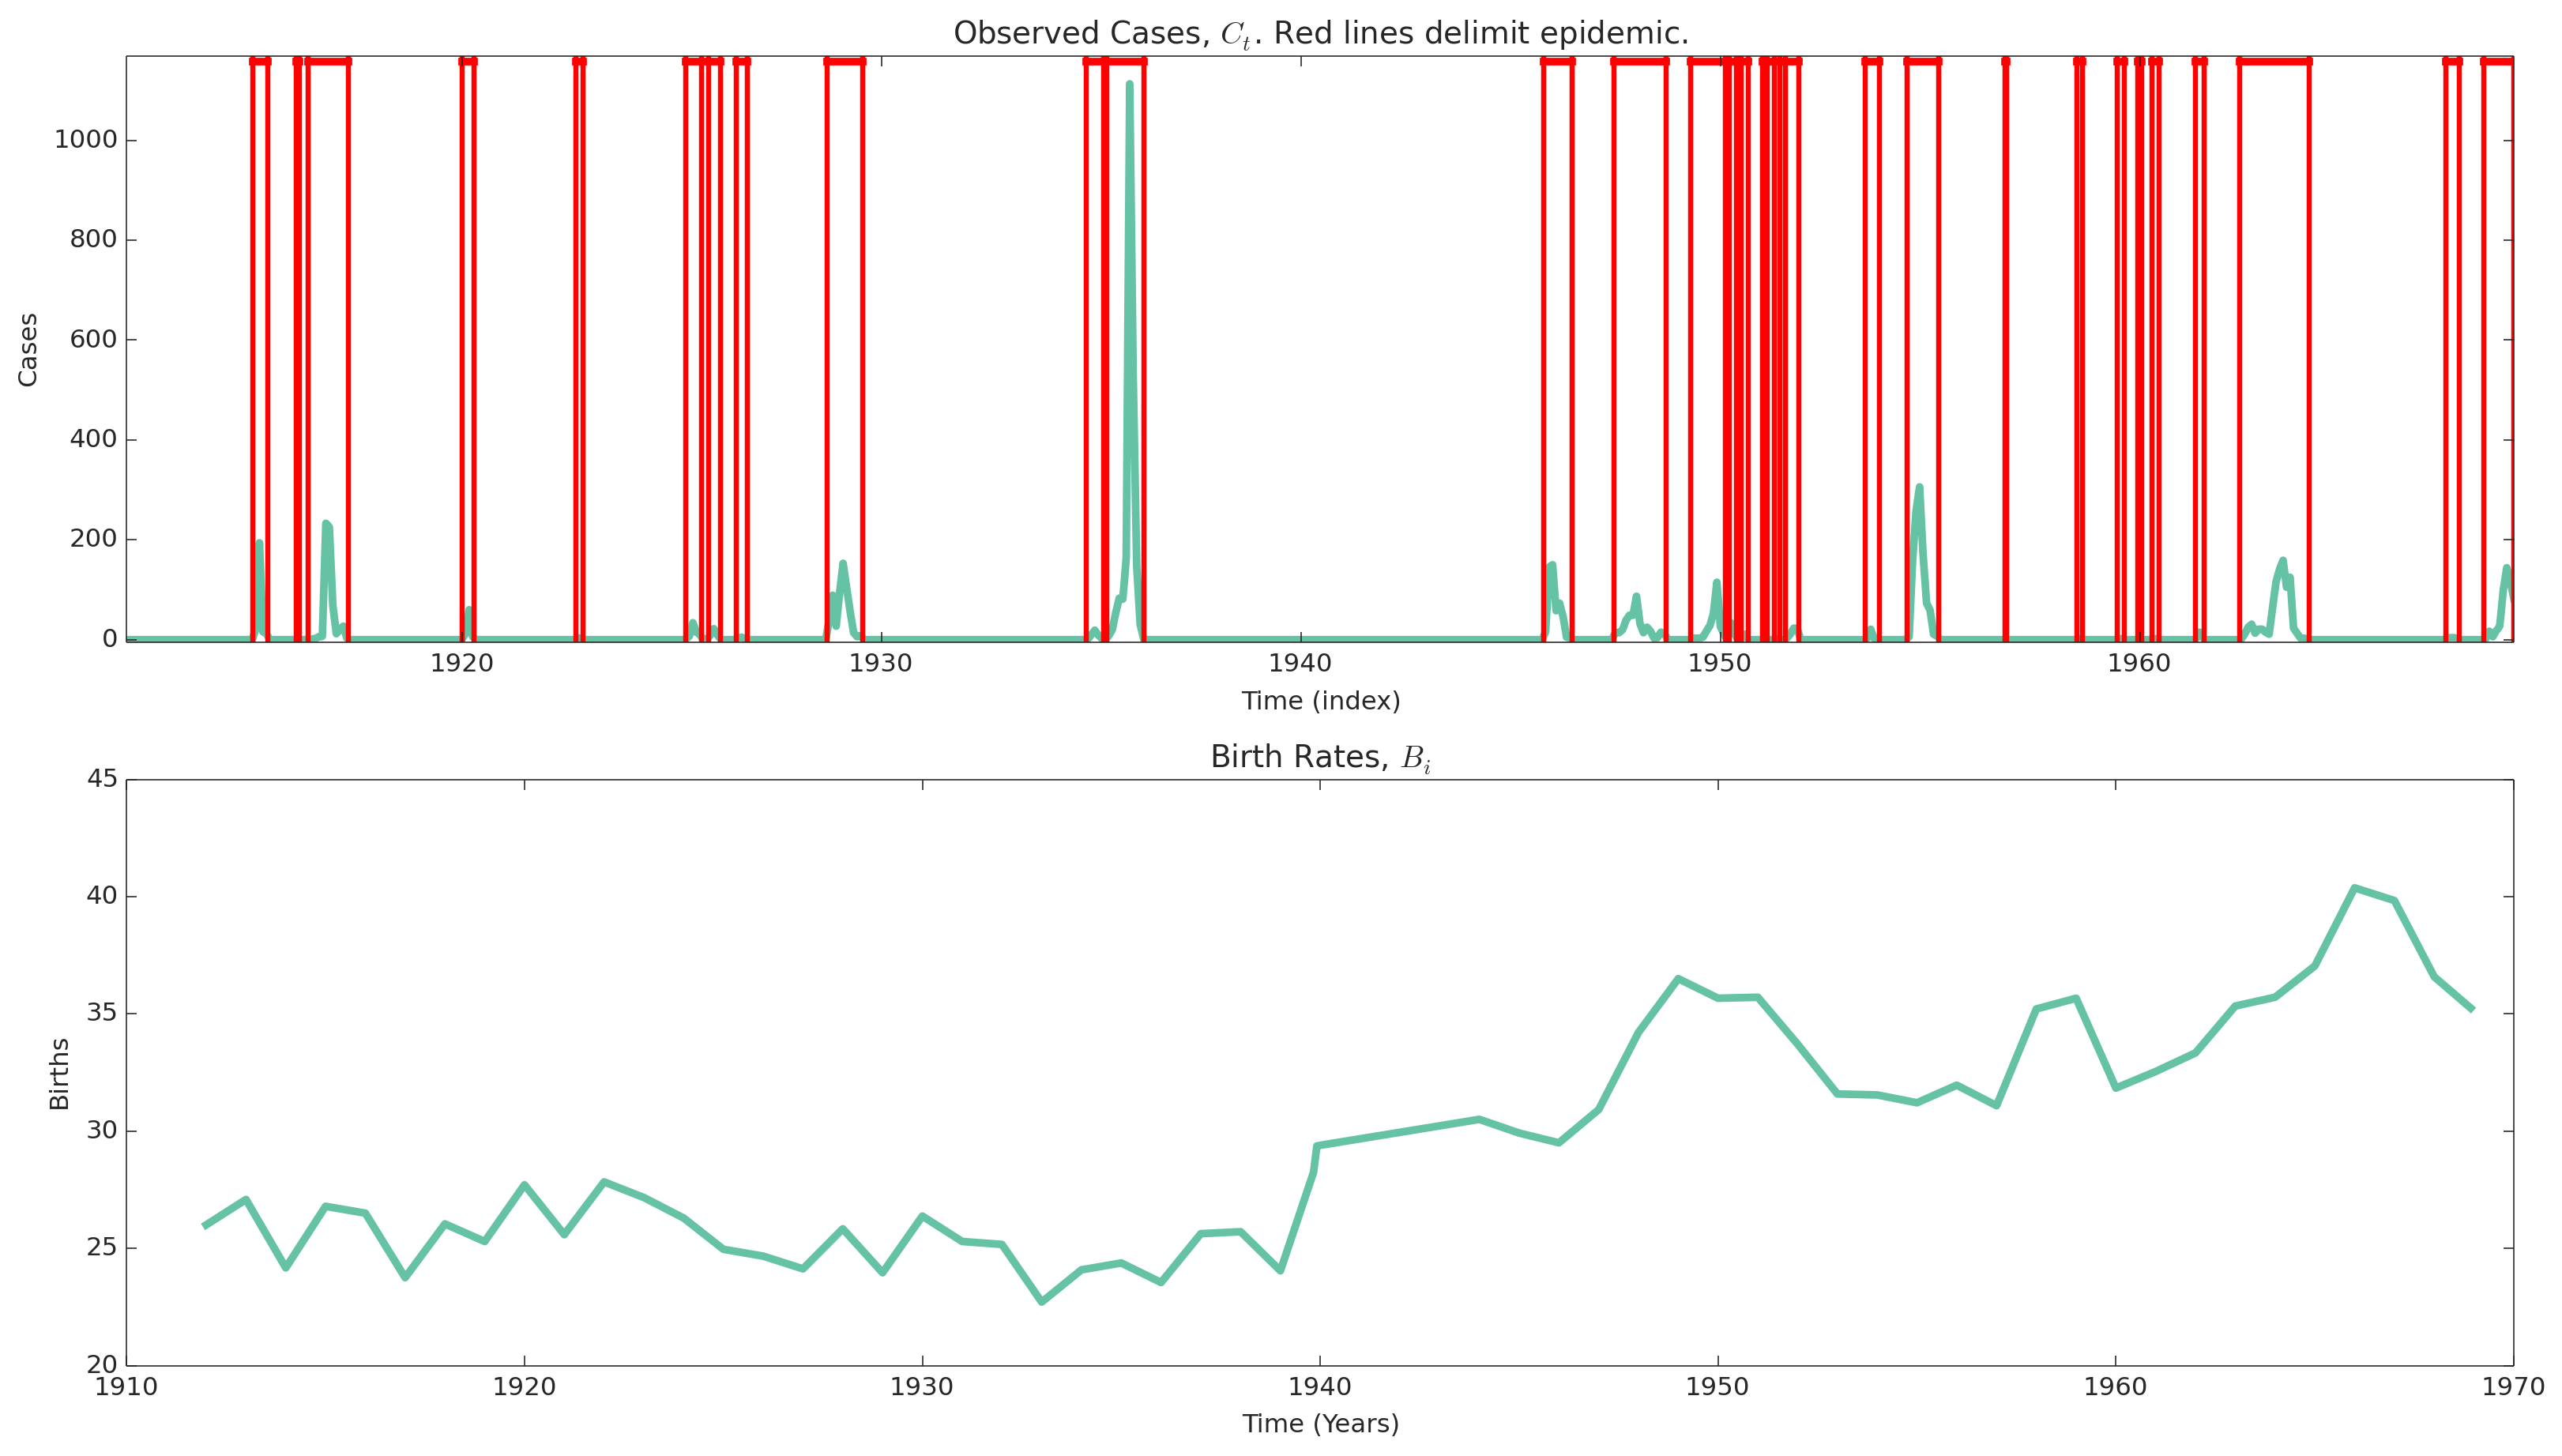
\includegraphics[max size={\textwidth}{\textheight}]{notebook_files/notebook_6_0.png}
    \par
    \end{center}
    
            \end{InvisibleVerbatim}
            
        
    


    % Make sure that atleast 4 lines are below the HR
    \needspace{4\baselineskip}

    
        \vspace{6pt}
        \makebox[0.1\linewidth]{\smaller\hfill\tt\color{nbframe-in-prompt}In\hspace{4pt}{[}13{]}:\hspace{4pt}}\\*
        \vspace{-2.65\baselineskip}
        \begin{ColorVerbatim}
            \vspace{-0.7\baselineskip}
            \begin{Verbatim}[commandchars=\\\{\}]
\PY{n}{np}\PY{o}{.}\PY{n}{sum}\PY{p}{(}\PY{n}{B}\PY{p}{)}
\end{Verbatim}

            
                \vspace{-0.2\baselineskip}
            
        \end{ColorVerbatim}
    

    

        % If the first block is an image, minipage the image.  Else
        % request a certain amount of space for the input text.
        \needspace{4\baselineskip}
        
        

            % Add document contents.
            
                \makebox[0.1\linewidth]{\smaller\hfill\tt\color{nbframe-out-prompt}Out\hspace{4pt}{[}13{]}:\hspace{4pt}}\\*
                \vspace{-2.55\baselineskip}\begin{InvisibleVerbatim}
                \vspace{-0.5\baselineskip}
\begin{alltt}40324.413507415979\end{alltt}

            \end{InvisibleVerbatim}
            
        
    
\textbf{Susceptible Reconstruction}

We have already defined $C$, the observed cases, and $B$, the
time-series of births. Reconstruction of the susceptible time-series
requires

\[
Y_t = \sum_{i=0}^t B_t, 
\] and \[
X_t = \sum_{i=0}^t C_t.
\]

This will enable us to find the true number of infected individuals :
$I_t = \rho_t \, C_t.$ Here, $\rho_t \ge 1$ is the linked to the
reporting rate by $1/\rho_t$.

We expand the number of susceptibles around its mean, as
$S_t = \bar{S} + Z_t$. Then, without repeating the results present in
the paper, we find that

\[
Y_t = -Z_0 + \rho_t \, X_t + Z_t.
\]

For constant $\rho$, this parameter could be fit using a simple linear
regression between the cumulative cases, $X_t$, and the cumulative
births, $Y_t$. The residuals of regression would then yield $Z_t$, the
dynamics of the susceptibles about their mean $\bar{S}$. When
$\rho = \rho_t$ is allowed to vary, a \emph{locally-linear} regression
must be used; this can be implemented in many ways, such as by fitting
piecewise-linear functions, splines, or the local polynomial regression
technique described in Fan and Gibjels (1996), as used in the paper by
Finkenstadt and Grenfell. Here, we use a polynomial, fitted by Bayesian
ridge regression, to calculate $\hat{Y}_t$, the estimator for $Y_t$, and
fit cubic splines to $\hat{Y}_t(X_t)$ to compute the slope of the
function, and hence, to find $\rho_t$.

    % Make sure that atleast 4 lines are below the HR
    \needspace{4\baselineskip}

    
        \vspace{6pt}
        \makebox[0.1\linewidth]{\smaller\hfill\tt\color{nbframe-in-prompt}In\hspace{4pt}{[}7{]}:\hspace{4pt}}\\*
        \vspace{-2.65\baselineskip}
        \begin{ColorVerbatim}
            \vspace{-0.7\baselineskip}
            \begin{Verbatim}[commandchars=\\\{\}]
\PY{c}{\PYZsh{} Susceptible Reconstruction}

\PY{c}{\PYZsh{} Compute cumulative births and incidence}
\PY{n}{Y} \PY{o}{=} \PY{n}{np}\PY{o}{.}\PY{n}{cumsum}\PY{p}{(}\PY{n}{B}\PY{p}{)}
\PY{n}{X} \PY{o}{=} \PY{n}{np}\PY{o}{.}\PY{n}{cumsum}\PY{p}{(}\PY{n}{C}\PY{p}{)} 


\PY{c}{\PYZsh{} Compute rho ( rate of reporting ) using Bayesian ridge regression with a polynomial}
\PY{n}{reg} \PY{o}{=} \PY{n}{linear\PYZus{}model}\PY{o}{.}\PY{n}{BayesianRidge}\PY{p}{(}\PY{n}{fit\PYZus{}intercept}\PY{o}{=}\PY{n+nb+bp}{False}\PY{p}{,} \PY{n}{compute\PYZus{}score}\PY{o}{=}\PY{n+nb+bp}{True}\PY{p}{)}

\PY{c}{\PYZsh{} Compute the R\PYZca{}2 for a range of polynomials from degree\PYZhy{}1 to degree\PYZhy{}10}
\PY{c}{\PYZsh{} The fit score has a penalty proportional to the square of the degree of the polynomial}
\PY{n}{Ns} \PY{o}{=} \PY{n+nb}{range}\PY{p}{(}\PY{l+m+mi}{2}\PY{p}{,} \PY{l+m+mi}{12}\PY{p}{)}
\PY{n}{scores} \PY{o}{=} \PY{p}{[}\PY{p}{]}
\PY{k}{for} \PY{n}{n} \PY{o+ow}{in} \PY{n}{Ns} \PY{p}{:}
    \PY{n}{reg}\PY{o}{.}\PY{n}{fit}\PY{p}{(}\PY{n}{np}\PY{o}{.}\PY{n}{vander}\PY{p}{(}\PY{n}{X}\PY{p}{,} \PY{n}{n}\PY{p}{)}\PY{p}{,} \PY{n}{Y}\PY{p}{)}
    \PY{n}{scores}\PY{o}{.}\PY{n}{append}\PY{p}{(}\PY{n}{reg}\PY{o}{.}\PY{n}{score}\PY{p}{(}\PY{n}{np}\PY{o}{.}\PY{n}{vander}\PY{p}{(}\PY{n}{X}\PY{p}{,} \PY{n}{n}\PY{p}{)}\PY{p}{,} \PY{n}{Y}\PY{p}{)} \PY{o}{\PYZhy{}} \PY{n}{penalty} \PY{o}{*} \PY{n}{n}\PY{o}{*}\PY{o}{*}\PY{l+m+mi}{2}\PY{p}{)}
    
\PY{c}{\PYZsh{} Use the polynomial that maximised R\PYZca{}2 to compute Yhat}
\PY{n}{Yhat} \PY{o}{=} \PY{n}{reg}\PY{o}{.}\PY{n}{fit}\PY{p}{(}\PY{n}{np}\PY{o}{.}\PY{n}{vander}\PY{p}{(}\PY{n}{X}\PY{p}{,} \PY{n}{Ns}\PY{p}{[}\PY{n}{np}\PY{o}{.}\PY{n}{argmax}\PY{p}{(}\PY{n}{scores}\PY{p}{)}\PY{p}{]}\PY{p}{)}\PY{p}{,} \PY{n}{Y}\PY{p}{)}\PY{o}{.}\PY{n}{predict}\PY{p}{(}\PY{n}{np}\PY{o}{.}\PY{n}{vander}\PY{p}{(}\PY{n}{X}\PY{p}{,} \PY{n}{Ns}\PY{p}{[}\PY{n}{np}\PY{o}{.}\PY{n}{argmax}\PY{p}{(}\PY{n}{scores}\PY{p}{)}\PY{p}{]}\PY{p}{)}\PY{p}{)}

\PY{c}{\PYZsh{} Compute rho as the derivative of the splines that are fit between X and the estimated Y}
\PY{n}{rho} \PY{o}{=} \PY{n}{interp}\PY{o}{.}\PY{n}{UnivariateSpline}\PY{p}{(}\PY{n}{X}\PY{p}{,} \PY{n}{Yhat}\PY{p}{)}\PY{o}{.}\PY{n}{derivative}\PY{p}{(}\PY{p}{)}\PY{p}{(}\PY{n}{X}\PY{p}{)}

\PY{c}{\PYZsh{} Compute Z as the residuals of regression}
\PY{n}{Z} \PY{o}{=} \PY{n}{Y} \PY{o}{\PYZhy{}} \PY{n}{Yhat}



\PY{c}{\PYZsh{} Plots}
\PY{n}{subplot}\PY{p}{(}\PY{l+m+mi}{221}\PY{p}{)}
\PY{n}{plt}\PY{o}{.}\PY{n}{plot}\PY{p}{(}\PY{n}{t}\PY{p}{,} \PY{n}{X}\PY{p}{,} \PY{n}{linewidth}\PY{o}{=}\PY{l+m+mi}{3}\PY{p}{)}
\PY{n}{plt}\PY{o}{.}\PY{n}{plot}\PY{p}{(}\PY{n}{t}\PY{p}{,} \PY{n}{Y}\PY{p}{,} \PY{n}{linewidth}\PY{o}{=}\PY{l+m+mi}{3}\PY{p}{)}
\PY{n}{plt}\PY{o}{.}\PY{n}{plot}\PY{p}{(}\PY{n}{t}\PY{p}{,} \PY{n}{Yhat}\PY{p}{,} \PY{n}{linewidth}\PY{o}{=}\PY{l+m+mi}{3}\PY{p}{)}
\PY{n}{title}\PY{p}{(}\PY{l+s}{\PYZdq{}}\PY{l+s}{Reported and Inferred Cases}\PY{l+s}{\PYZdq{}}\PY{p}{)}
\PY{n}{legend}\PY{p}{(}\PY{p}{[}\PY{l+s}{\PYZdq{}}\PY{l+s}{Reported Cases}\PY{l+s}{\PYZdq{}}\PY{p}{,} \PY{l+s}{\PYZdq{}}\PY{l+s}{Cumulative Births}\PY{l+s}{\PYZdq{}}\PY{p}{,} \PY{l+s}{\PYZdq{}}\PY{l+s}{Inferred Cases}\PY{l+s}{\PYZdq{}}\PY{p}{]}\PY{p}{,} \PY{n}{loc}\PY{o}{=}\PY{l+m+mi}{2}\PY{p}{)}

\PY{n}{subplot}\PY{p}{(}\PY{l+m+mi}{222}\PY{p}{)}
\PY{n}{axhline}\PY{p}{(}\PY{l+m+mf}{1.}\PY{o}{/}\PY{n}{np}\PY{o}{.}\PY{n}{mean}\PY{p}{(}\PY{n}{rho}\PY{p}{)}\PY{p}{,} \PY{n}{color}\PY{o}{=}\PY{l+s}{\PYZdq{}}\PY{l+s}{r}\PY{l+s}{\PYZdq{}}\PY{p}{,} \PY{n}{linewidth}\PY{o}{=}\PY{l+m+mi}{2}\PY{p}{)}
\PY{n}{plt}\PY{o}{.}\PY{n}{plot}\PY{p}{(}\PY{n}{t}\PY{p}{,} \PY{l+m+mf}{1.}\PY{o}{/}\PY{n}{rho}\PY{p}{,} \PY{n}{linewidth}\PY{o}{=}\PY{l+m+mi}{3}\PY{p}{)}
\PY{n}{ylim}\PY{p}{(}\PY{p}{[}\PY{l+m+mi}{0}\PY{p}{,} \PY{l+m+mi}{1}\PY{p}{]}\PY{p}{)}
\PY{n}{title}\PY{p}{(}\PY{l+s}{r\PYZdq{}}\PY{l+s}{Inferred Reporting Rate \PYZdl{}1/}\PY{l+s}{\PYZbs{}}\PY{l+s}{rho\PYZus{}t\PYZdl{}}\PY{l+s}{\PYZdq{}}\PY{p}{)}
\PY{n}{legend}\PY{p}{(}\PY{p}{[}\PY{l+s}{r\PYZdq{}}\PY{l+s}{\PYZdl{}E[1/}\PY{l+s}{\PYZbs{}}\PY{l+s}{rho\PYZus{}t]=\PYZdl{}}\PY{l+s}{\PYZdq{}} \PY{o}{+} \PY{n+nb}{str}\PY{p}{(}\PY{l+m+mf}{1.}\PY{o}{/}\PY{n}{np}\PY{o}{.}\PY{n}{mean}\PY{p}{(}\PY{n}{rho}\PY{p}{)}\PY{p}{)}\PY{p}{]}\PY{p}{)}

\PY{n}{subplot}\PY{p}{(}\PY{l+m+mi}{223}\PY{p}{)}
\PY{n}{plt}\PY{o}{.}\PY{n}{plot}\PY{p}{(}\PY{n}{t}\PY{p}{,} \PY{n}{Z}\PY{p}{,} \PY{n}{linewidth}\PY{o}{=}\PY{l+m+mi}{3}\PY{p}{)}
\PY{n}{title}\PY{p}{(}\PY{l+s}{\PYZdq{}}\PY{l+s}{Susceptible Dynamics \PYZdl{}Z\PYZus{}t\PYZdl{}}\PY{l+s}{\PYZdq{}}\PY{p}{)}
\PY{n}{xlabel}\PY{p}{(}\PY{l+s}{\PYZdq{}}\PY{l+s}{Time (years)}\PY{l+s}{\PYZdq{}}\PY{p}{)}

\PY{n}{subplot}\PY{p}{(}\PY{l+m+mi}{224}\PY{p}{)}
\PY{n}{plt}\PY{o}{.}\PY{n}{plot}\PY{p}{(}\PY{n}{np}\PY{o}{.}\PY{n}{array}\PY{p}{(}\PY{n}{Ns}\PY{p}{)}\PY{o}{\PYZhy{}}\PY{l+m+mi}{1}\PY{p}{,} \PY{n}{scores}\PY{p}{,} \PY{n}{linewidth}\PY{o}{=}\PY{l+m+mi}{3}\PY{p}{)}
\PY{n}{axvline}\PY{p}{(}\PY{n}{Ns}\PY{p}{[}\PY{n}{np}\PY{o}{.}\PY{n}{argmax}\PY{p}{(}\PY{n}{scores}\PY{p}{)}\PY{p}{]}\PY{o}{\PYZhy{}}\PY{l+m+mi}{1}\PY{p}{,} \PY{n}{color}\PY{o}{=}\PY{l+s}{\PYZdq{}}\PY{l+s}{r}\PY{l+s}{\PYZdq{}}\PY{p}{,} \PY{n}{linewidth}\PY{o}{=}\PY{l+m+mi}{2}\PY{p}{)}
\PY{n}{title}\PY{p}{(}\PY{l+s}{\PYZdq{}}\PY{l+s}{Polynomial Model Fit, n = }\PY{l+s}{\PYZdq{}} \PY{o}{+} \PY{n+nb}{str}\PY{p}{(}\PY{n}{Ns}\PY{p}{[}\PY{n}{np}\PY{o}{.}\PY{n}{argmax}\PY{p}{(}\PY{n}{scores}\PY{p}{)}\PY{p}{]}\PY{o}{\PYZhy{}}\PY{l+m+mi}{1}\PY{p}{)}\PY{p}{)}
\PY{n}{xlabel}\PY{p}{(}\PY{l+s}{\PYZdq{}}\PY{l+s}{Polynomial Degree}\PY{l+s}{\PYZdq{}}\PY{p}{)}
\PY{n}{ylabel}\PY{p}{(}\PY{l+s}{\PYZdq{}}\PY{l+s}{Penalised Goodness of Fit}\PY{l+s}{\PYZdq{}}\PY{p}{)}
\end{Verbatim}

            
                \vspace{-0.2\baselineskip}
            
        \end{ColorVerbatim}
    

    

        % If the first block is an image, minipage the image.  Else
        % request a certain amount of space for the input text.
        \needspace{4\baselineskip}
        
        

            % Add document contents.
            
                \makebox[0.1\linewidth]{\smaller\hfill\tt\color{nbframe-out-prompt}Out\hspace{4pt}{[}7{]}:\hspace{4pt}}\\*
                \vspace{-2.55\baselineskip}\begin{InvisibleVerbatim}
                \vspace{-0.5\baselineskip}
\begin{alltt}<matplotlib.text.Text at 0x10d30b110>\end{alltt}

            \end{InvisibleVerbatim}
            
                \begin{InvisibleVerbatim}
                \vspace{-0.5\baselineskip}
    \begin{center}
    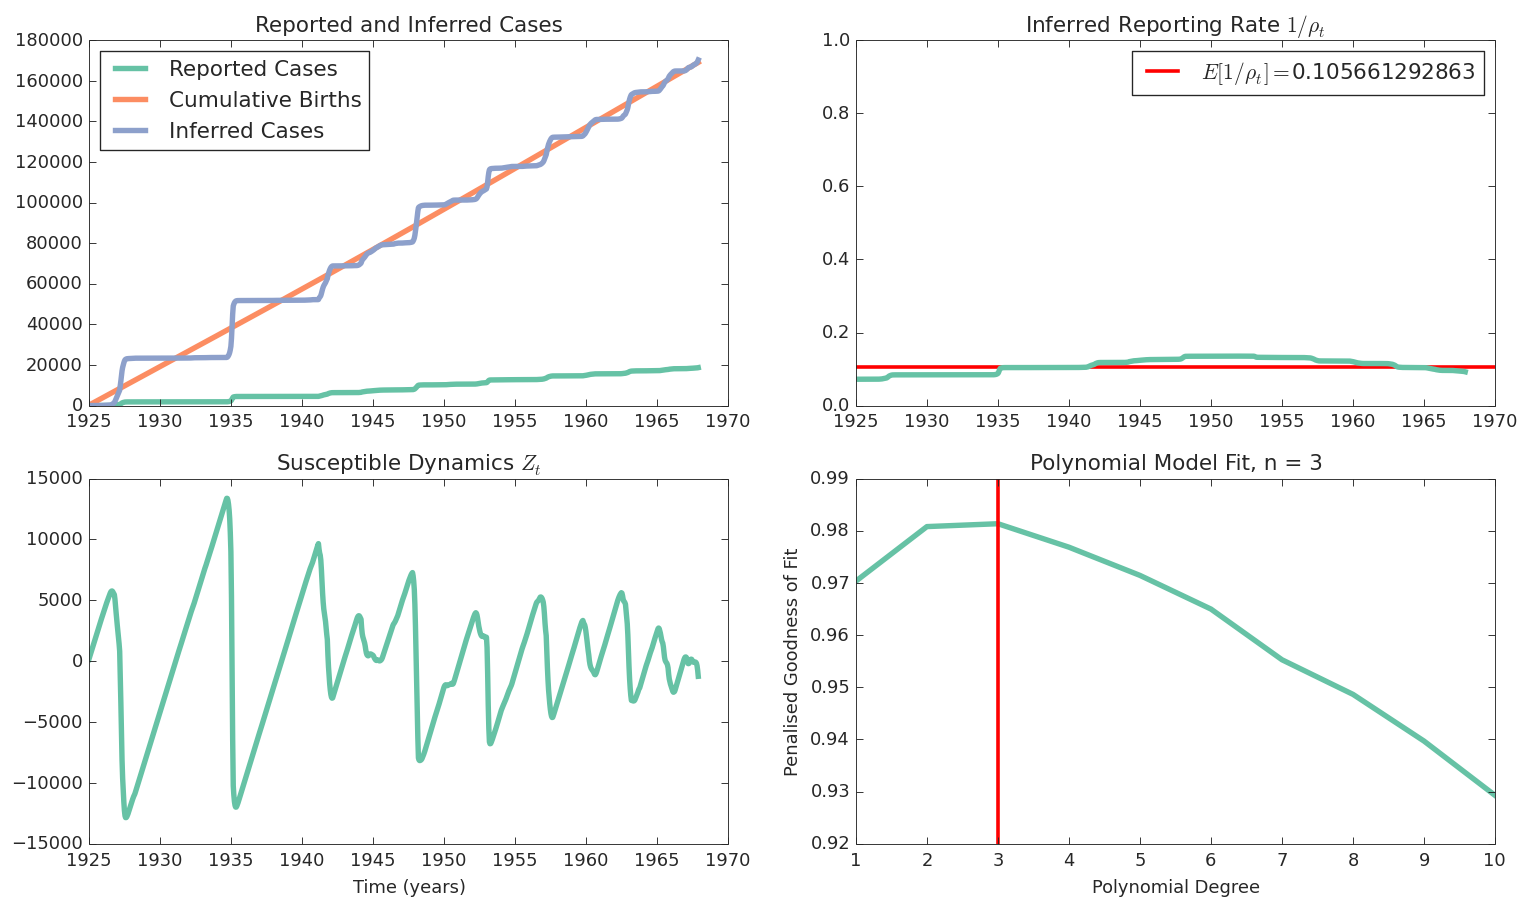
\includegraphics[max size={\textwidth}{\textheight}]{notebook_files/notebook_9_1.png}
    \par
    \end{center}
    
            \end{InvisibleVerbatim}
            
        
    
\textbf{Parameter Inference}

With the susceptible dynamics $Z_t$ reconstructed, we can infer the
contact rate, $r_t$, and the homogeneity parameter, $\alpha$. To do
this, we take logarithms of the main equations of the TSIR model :

\[
\ln(I_{t+1}) = \ln(r_t) + \alpha \ln(I_t) + \ln(S_t),
\] \[
\ln(S_{t+1}) = \ln(B_{t-d}) + \ln(S_t) - \ln(I_t),
\]

after dropping the noise terms. We first impose that $r_t$ be periodic
with a period of one year; if we denote $P$ as the number of time points
in one year, then we impose that
$r_{t\,+\,n\,P} = r_t \; \forall \; n \in \mathrm{Z}^+$. Instead of
assuming a sinusoidal forcing, Finkenstadt and Grenfell allow $r_t$ to
be as general as possible, effectively making the periodic function into
a series of $P$ parameters $r_0, \,\dots,\, r_{P-1}$.

Then, we must find a way to compute $\ln(S_t)$. We take a Taylor
expansion, approximating this term as

\[
\ln(S_t) = \ln(\bar{S}+Z_t) \approx \ln(\bar{S}) + \frac{Z_t}{\bar{S}}.
\]

Substituting this into the previous equation for the number of infected
individuals, we find that

\[
\ln(I_{t+1}) = \ln(\bar{S}\,r_t) + \alpha \ln(I_t) + \frac{Z_t}{\bar{S}}.
\]

Here, we use this approximation to infer the homogeneity parameter,
$\alpha$; the mean number of susceptibles, $\bar{S}$; and hence, the $P$
contact rate parameters, $r_t$, having inferred $\bar{S}\,r_t$.

    % Make sure that atleast 4 lines are below the HR
    \needspace{4\baselineskip}

    
        \vspace{6pt}
        \makebox[0.1\linewidth]{\smaller\hfill\tt\color{nbframe-in-prompt}In\hspace{4pt}{[}248{]}:\hspace{4pt}}\\*
        \vspace{-2.65\baselineskip}
        \begin{ColorVerbatim}
            \vspace{-0.7\baselineskip}
            \begin{Verbatim}[commandchars=\\\{\}]
\PY{c}{\PYZsh{} EQUATION 15}

\PY{c}{\PYZsh{} Fit a linear model to infer periodicity, alpha, and Sbar \PYZhy{} using Z only}

\PY{c}{\PYZsh{} Allocate design matrix}
\PY{n}{A} \PY{o}{=} \PY{n}{np}\PY{o}{.}\PY{n}{zeros}\PY{p}{(}\PY{p}{(}\PY{n+nb}{len}\PY{p}{(}\PY{n}{z}\PY{p}{)}\PY{o}{\PYZhy{}}\PY{l+m+mi}{1}\PY{p}{,} \PY{n}{periodicity}\PY{o}{+}\PY{l+m+mi}{2}\PY{p}{)}\PY{p}{)}

\PY{c}{\PYZsh{} Periodicity indicators for the design matrix}
\PY{k}{for} \PY{n}{i} \PY{o+ow}{in} \PY{n+nb}{range}\PY{p}{(}\PY{n+nb}{len}\PY{p}{(}\PY{n}{z}\PY{p}{)}\PY{o}{\PYZhy{}}\PY{l+m+mi}{1}\PY{p}{)} \PY{p}{:}
    \PY{n}{A}\PY{p}{[}\PY{n}{i}\PY{p}{,} \PY{n}{i} \PY{o}{\PYZpc{}} \PY{n}{periodicity}\PY{p}{]} \PY{o}{=} \PY{l+m+mi}{1}

\PY{c}{\PYZsh{} Set I(t\PYZhy{}1), Z(t\PYZhy{}1)}
\PY{n}{A}\PY{p}{[}\PY{p}{:}\PY{p}{,} \PY{n}{periodicity}\PY{p}{]} \PY{o}{=} \PY{n}{np}\PY{o}{.}\PY{n}{log}\PY{p}{(}\PY{n}{rho}\PY{p}{[}\PY{n}{z}\PY{p}{[}\PY{p}{:}\PY{o}{\PYZhy{}}\PY{l+m+mi}{1}\PY{p}{]}\PY{p}{]} \PY{o}{*} \PY{n}{C}\PY{p}{[}\PY{n}{z}\PY{p}{[}\PY{p}{:}\PY{o}{\PYZhy{}}\PY{l+m+mi}{1}\PY{p}{]}\PY{p}{]}\PY{p}{)}
\PY{n}{A}\PY{p}{[}\PY{p}{:}\PY{p}{,} \PY{n}{periodicity}\PY{o}{+}\PY{l+m+mi}{1}\PY{p}{]} \PY{o}{=} \PY{n}{Z}\PY{p}{[}\PY{n}{z}\PY{p}{[}\PY{p}{:}\PY{o}{\PYZhy{}}\PY{l+m+mi}{1}\PY{p}{]}\PY{p}{]}



\PY{c}{\PYZsh{} Initialise results vector}
\PY{n}{y} \PY{o}{=} \PY{n}{np}\PY{o}{.}\PY{n}{log}\PY{p}{(}\PY{n}{rho}\PY{p}{[}\PY{n}{z}\PY{p}{[}\PY{l+m+mi}{1}\PY{p}{:}\PY{p}{]}\PY{p}{]} \PY{o}{*} \PY{n}{C}\PY{p}{[}\PY{n}{z}\PY{p}{[}\PY{l+m+mi}{1}\PY{p}{:}\PY{p}{]}\PY{p}{]}\PY{p}{)}



\PY{c}{\PYZsh{} Infer parameters using Bayesian ridge regression}
\PY{n}{reg2} \PY{o}{=} \PY{n}{linear\PYZus{}model}\PY{o}{.}\PY{n}{BayesianRidge}\PY{p}{(}\PY{n}{fit\PYZus{}intercept}\PY{o}{=}\PY{n+nb+bp}{False}\PY{p}{)}
\PY{n}{reg2}\PY{o}{.}\PY{n}{fit}\PY{p}{(}\PY{n}{A}\PY{p}{,} \PY{n}{y}\PY{p}{)}


\PY{c}{\PYZsh{} Extract useful parameters}
\PY{n}{rstar} \PY{o}{=} \PY{n}{np}\PY{o}{.}\PY{n}{exp}\PY{p}{(}\PY{n}{reg2}\PY{o}{.}\PY{n}{coef\PYZus{}}\PY{p}{[}\PY{p}{:}\PY{n}{periodicity}\PY{p}{]}\PY{p}{)} \PY{c}{\PYZsh{} Sbar * r\PYZus{}t}
\PY{n}{alphaZ} \PY{o}{=} \PY{n}{reg2}\PY{o}{.}\PY{n}{coef\PYZus{}}\PY{p}{[}\PY{n}{periodicity}\PY{p}{]} \PY{c}{\PYZsh{} alpha}
\PY{n}{zeta} \PY{o}{=} \PY{n}{reg2}\PY{o}{.}\PY{n}{coef\PYZus{}}\PY{p}{[}\PY{n}{periodicity}\PY{o}{+}\PY{l+m+mi}{1}\PY{p}{]} \PY{c}{\PYZsh{} Sbar}

\PY{c}{\PYZsh{}plt.plot(rstar, linewidth=2)}
\PY{c}{\PYZsh{}title(\PYZdq{}Periodicity\PYZdq{})}
\PY{k}{print} \PY{l+s}{\PYZdq{}}\PY{l+s}{Alpha = }\PY{l+s}{\PYZdq{}} \PY{o}{+} \PY{n+nb}{str}\PY{p}{(}\PY{n}{alphaZ}\PY{p}{)}
\PY{k}{print} \PY{l+s}{\PYZdq{}}\PY{l+s}{Sbar = }\PY{l+s}{\PYZdq{}} \PY{o}{+} \PY{n+nb}{str}\PY{p}{(}\PY{l+m+mf}{1.}\PY{o}{/}\PY{n}{zeta}\PY{p}{)}
\PY{k}{if} \PY{o+ow}{not} \PY{p}{(}\PY{n}{LONDON} \PY{o+ow}{or} \PY{n}{ICELAND} \PY{o+ow}{or} \PY{n}{FAROE} \PY{o+ow}{or} \PY{n}{BORNHOLM}\PY{p}{)} \PY{p}{:}
    \PY{k}{print} \PY{l+s}{\PYZdq{}}\PY{l+s}{Real Sbar = }\PY{l+s}{\PYZdq{}} \PY{o}{+} \PY{n+nb}{str}\PY{p}{(}\PY{n}{np}\PY{o}{.}\PY{n}{mean}\PY{p}{(}\PY{n}{S}\PY{p}{)}\PY{p}{)}
    \PY{k}{print} \PY{l+s}{\PYZdq{}}\PY{l+s}{Error in Sbar prediction = }\PY{l+s}{\PYZdq{}} \PY{o}{+} \PY{n+nb}{str}\PY{p}{(}\PY{l+m+mi}{100}\PY{o}{*}\PY{n}{np}\PY{o}{.}\PY{n}{abs}\PY{p}{(}\PY{l+m+mf}{1.}\PY{o}{/}\PY{n}{zeta} \PY{o}{\PYZhy{}} \PY{n}{np}\PY{o}{.}\PY{n}{mean}\PY{p}{(}\PY{n}{S}\PY{p}{)}\PY{p}{)}\PY{o}{/}\PY{n}{np}\PY{o}{.}\PY{n}{mean}\PY{p}{(}\PY{n}{S}\PY{p}{)}\PY{p}{)} \PY{o}{+} \PY{n+nb}{str}\PY{p}{(}\PY{l+s}{\PYZdq{}}\PY{l+s}{ }\PY{l+s}{\PYZpc{}}\PY{l+s}{\PYZdq{}}\PY{p}{)}
\end{Verbatim}

            
                \vspace{-0.2\baselineskip}
            
        \end{ColorVerbatim}
    

    

        % If the first block is an image, minipage the image.  Else
        % request a certain amount of space for the input text.
        \needspace{4\baselineskip}
        
        

            % Add document contents.
            
                \begin{InvisibleVerbatim}
                \vspace{-0.5\baselineskip}
\begin{alltt}Alpha = 0.971414089617
Sbar = 8440.35832034
\end{alltt}

            \end{InvisibleVerbatim}
            
        
    
\textbf{Parameter Inference 2}

Instead of using the Taylor expansion of $\ln(\bar{S} + Z_t)$, we can
estimate $\ln(\bar{S})$ by finding the value of $\bar{S}$ that maximises
the likelihood of the main equation.

    % Make sure that atleast 4 lines are below the HR
    \needspace{4\baselineskip}

    
        \vspace{6pt}
        \makebox[0.1\linewidth]{\smaller\hfill\tt\color{nbframe-in-prompt}In\hspace{4pt}{[}249{]}:\hspace{4pt}}\\*
        \vspace{-2.65\baselineskip}
        \begin{ColorVerbatim}
            \vspace{-0.7\baselineskip}
            \begin{Verbatim}[commandchars=\\\{\}]
\PY{c}{\PYZsh{} EQUATION 12}

\PY{c}{\PYZsh{} All possible values of Sbar}
\PY{n}{Svals} \PY{o}{=} \PY{n}{np}\PY{o}{.}\PY{n}{linspace}\PY{p}{(}\PY{n}{np}\PY{o}{.}\PY{n}{abs}\PY{p}{(}\PY{n}{np}\PY{o}{.}\PY{n}{min}\PY{p}{(}\PY{n}{Z}\PY{p}{)}\PY{p}{)}\PY{o}{+}\PY{l+m+mi}{1}\PY{p}{,} \PY{n}{np}\PY{o}{.}\PY{n}{abs}\PY{p}{(}\PY{n}{np}\PY{o}{.}\PY{n}{min}\PY{p}{(}\PY{n}{Z}\PY{p}{)}\PY{p}{)}\PY{o}{*}\PY{l+m+mi}{13}\PY{p}{,} \PY{l+m+mi}{100}\PY{p}{)}


\PY{c}{\PYZsh{} Likelihood of fit}
\PY{n}{l} \PY{o}{=} \PY{n}{np}\PY{o}{.}\PY{n}{zeros}\PY{p}{(}\PY{n+nb}{len}\PY{p}{(}\PY{n}{Svals}\PY{p}{)}\PY{p}{)}


\PY{c}{\PYZsh{} Define our parameters}
\PY{n}{params} \PY{o}{=} \PY{n}{lmfit}\PY{o}{.}\PY{n}{Parameters}\PY{p}{(}\PY{p}{)}
\PY{n}{params}\PY{o}{.}\PY{n}{add}\PY{p}{(}\PY{l+s}{\PYZdq{}}\PY{l+s}{alpha}\PY{l+s}{\PYZdq{}}\PY{p}{,} \PY{n+nb}{min}\PY{o}{=}\PY{l+m+mf}{0.5}\PY{p}{,} \PY{n+nb}{max}\PY{o}{=}\PY{l+m+mf}{1.}\PY{p}{,} \PY{n}{value}\PY{o}{=}\PY{l+m+mf}{0.95}\PY{p}{)} \PY{c}{\PYZsh{} Alpha}
\PY{k}{for} \PY{n}{i} \PY{o+ow}{in} \PY{n+nb}{range}\PY{p}{(}\PY{n}{periodicity}\PY{p}{)} \PY{p}{:} \PY{c}{\PYZsh{} Seasonalities}
    \PY{n}{params}\PY{o}{.}\PY{n}{add}\PY{p}{(}\PY{l+s}{\PYZdq{}}\PY{l+s}{r}\PY{l+s}{\PYZdq{}} \PY{o}{+} \PY{n+nb}{str}\PY{p}{(}\PY{n}{i}\PY{p}{)}\PY{p}{,} \PY{n}{value}\PY{o}{=}\PY{l+m+mf}{0.}\PY{p}{)}
\PY{n}{rstr} \PY{o}{=} \PY{p}{[}\PY{l+s}{\PYZdq{}}\PY{l+s}{r}\PY{l+s}{\PYZdq{}} \PY{o}{+} \PY{n+nb}{str}\PY{p}{(}\PY{n}{i} \PY{o}{\PYZpc{}} \PY{n}{periodicity}\PY{p}{)} \PY{k}{for} \PY{n}{i} \PY{o+ow}{in} \PY{n+nb}{list}\PY{p}{(}\PY{n}{itertools}\PY{o}{.}\PY{n}{chain}\PY{o}{.}\PY{n}{from\PYZus{}iterable}\PY{p}{(}\PY{n}{epi}\PY{p}{)}\PY{p}{)}\PY{p}{]}\PY{p}{[}\PY{p}{:}\PY{o}{\PYZhy{}}\PY{l+m+mi}{1}\PY{p}{]}
\PY{c}{\PYZsh{}if }
    
\PY{c}{\PYZsh{} Objective function}
\PY{k}{def} \PY{n+nf}{profile\PYZus{}residuals}\PY{p}{(}\PY{n}{params}\PY{p}{,} \PY{n}{rho}\PY{p}{,} \PY{n}{C}\PY{p}{,} \PY{n}{Z}\PY{p}{,} \PY{n}{z}\PY{p}{,} \PY{n}{Sestimate}\PY{p}{)} \PY{p}{:}
    \PY{n}{alphafit} \PY{o}{=} \PY{n}{params}\PY{p}{[}\PY{l+s}{\PYZdq{}}\PY{l+s}{alpha}\PY{l+s}{\PYZdq{}}\PY{p}{]}\PY{o}{.}\PY{n}{value}
    \PY{n}{r} \PY{o}{=} \PY{p}{[}\PY{n}{params}\PY{p}{[}\PY{n}{i}\PY{p}{]}\PY{o}{.}\PY{n}{value} \PY{k}{for} \PY{n}{i} \PY{o+ow}{in} \PY{n}{rstr}\PY{p}{]}
    \PY{k}{if} \PY{n}{isnan}\PY{p}{(}\PY{n}{Sestimate}\PY{p}{)} \PY{p}{:}
        \PY{n}{Sestimate} \PY{o}{=} \PY{n}{params}\PY{p}{[}\PY{l+s}{\PYZdq{}}\PY{l+s}{Sest}\PY{l+s}{\PYZdq{}}\PY{p}{]}\PY{o}{.}\PY{n}{value}
    \PY{k}{return} \PY{n}{alphafit} \PY{o}{*} \PY{n}{np}\PY{o}{.}\PY{n}{log}\PY{p}{(}\PY{n}{rho}\PY{p}{[}\PY{n}{z}\PY{p}{[}\PY{p}{:}\PY{o}{\PYZhy{}}\PY{l+m+mi}{1}\PY{p}{]}\PY{p}{]}\PY{o}{*}\PY{n}{C}\PY{p}{[}\PY{n}{z}\PY{p}{[}\PY{p}{:}\PY{o}{\PYZhy{}}\PY{l+m+mi}{1}\PY{p}{]}\PY{p}{]}\PY{p}{)} \PY{o}{+} \PY{n}{r} \PY{o}{+} \PY{n}{np}\PY{o}{.}\PY{n}{log}\PY{p}{(}\PY{n}{Sestimate} \PY{o}{+} \PY{n}{Z}\PY{p}{[}\PY{n}{z}\PY{p}{[}\PY{p}{:}\PY{o}{\PYZhy{}}\PY{l+m+mi}{1}\PY{p}{]}\PY{p}{]}\PY{p}{)} \PY{o}{\PYZhy{}} \PY{n}{np}\PY{o}{.}\PY{n}{log}\PY{p}{(}\PY{n}{rho}\PY{p}{[}\PY{n}{z}\PY{p}{[}\PY{l+m+mi}{1}\PY{p}{:}\PY{p}{]}\PY{p}{]}\PY{o}{*}\PY{n}{C}\PY{p}{[}\PY{n}{z}\PY{p}{[}\PY{l+m+mi}{1}\PY{p}{:}\PY{p}{]}\PY{p}{]}\PY{p}{)}
    

    
    
    
    
    
\PY{c}{\PYZsh{} Compute best fit for each possible Sbar}
\PY{k}{for} \PY{n}{i}\PY{p}{,} \PY{n}{Sestimate} \PY{o+ow}{in} \PY{n+nb}{enumerate}\PY{p}{(}\PY{n}{Svals}\PY{p}{)} \PY{p}{:}
    \PY{n}{l}\PY{p}{[}\PY{n}{i}\PY{p}{]} \PY{o}{=} \PY{n}{lmfit}\PY{o}{.}\PY{n}{minimize}\PY{p}{(}\PY{n}{profile\PYZus{}residuals}\PY{p}{,} \PY{n}{params}\PY{p}{,} \PY{n}{args}\PY{o}{=}\PY{p}{(}\PY{n}{rho}\PY{p}{,} \PY{n}{C}\PY{p}{,} \PY{n}{Z}\PY{p}{,} \PY{n}{z}\PY{p}{,} \PY{n}{Sestimate}\PY{p}{)}\PY{p}{,} \PY{n}{method}\PY{o}{=}\PY{l+s}{\PYZdq{}}\PY{l+s}{leastsq}\PY{l+s}{\PYZdq{}}\PY{p}{)}\PY{o}{.}\PY{n}{chisqr}
    
    
\PY{c}{\PYZsh{} Fit window}
\PY{n}{fitwindow} \PY{o}{=} \PY{l+m+mi}{15}
\PY{n}{fitwindowL} \PY{o}{=} \PY{n}{np}\PY{o}{.}\PY{n}{min}\PY{p}{(}\PY{p}{[}\PY{n}{fitwindow}\PY{p}{,} \PY{n}{np}\PY{o}{.}\PY{n}{argmin}\PY{p}{(}\PY{n}{l}\PY{p}{)}\PY{p}{]}\PY{p}{)}
\PY{n}{fitwindowR} \PY{o}{=} \PY{n}{np}\PY{o}{.}\PY{n}{min}\PY{p}{(}\PY{p}{[}\PY{n}{fitwindow}\PY{p}{,} \PY{n+nb}{len}\PY{p}{(}\PY{n}{Svals}\PY{p}{)} \PY{o}{\PYZhy{}} \PY{n}{np}\PY{o}{.}\PY{n}{argmin}\PY{p}{(}\PY{n}{l}\PY{p}{)}\PY{p}{]}\PY{p}{)}
    
\PY{c}{\PYZsh{} Run again using scan estimate}
\PY{n}{params}\PY{o}{.}\PY{n}{add}\PY{p}{(}\PY{l+s}{\PYZdq{}}\PY{l+s}{Sest}\PY{l+s}{\PYZdq{}}\PY{p}{,} \PY{n}{value} \PY{o}{=} \PY{n}{Svals}\PY{p}{[}\PY{n}{np}\PY{o}{.}\PY{n}{argmin}\PY{p}{(}\PY{n}{l}\PY{p}{)}\PY{p}{]}\PY{p}{)}
\PY{n}{L} \PY{o}{=} \PY{n}{lmfit}\PY{o}{.}\PY{n}{minimize}\PY{p}{(}\PY{n}{profile\PYZus{}residuals}\PY{p}{,} \PY{n}{params}\PY{p}{,} \PY{n}{args}\PY{o}{=}\PY{p}{(}\PY{n}{rho}\PY{p}{,} \PY{n}{C}\PY{p}{,} \PY{n}{Z}\PY{p}{,} \PY{n}{z}\PY{p}{,} \PY{n}{np}\PY{o}{.}\PY{n}{nan}\PY{p}{)}\PY{p}{,} \PY{n}{method}\PY{o}{=}\PY{l+s}{\PYZdq{}}\PY{l+s}{leastsq}\PY{l+s}{\PYZdq{}}\PY{p}{)}


\PY{c}{\PYZsh{} Extract parameters and errors}
\PY{n}{Sbar} \PY{o}{=} \PY{n}{L}\PY{o}{.}\PY{n}{params}\PY{p}{[}\PY{l+s}{\PYZdq{}}\PY{l+s}{Sest}\PY{l+s}{\PYZdq{}}\PY{p}{]}\PY{o}{.}\PY{n}{value}
\PY{n}{r} \PY{o}{=} \PY{n}{np}\PY{o}{.}\PY{n}{exp}\PY{p}{(}\PY{p}{[}\PY{n}{L}\PY{o}{.}\PY{n}{params}\PY{p}{[}\PY{l+s}{\PYZdq{}}\PY{l+s}{r}\PY{l+s}{\PYZdq{}} \PY{o}{+} \PY{n+nb}{str}\PY{p}{(}\PY{n}{i}\PY{p}{)}\PY{p}{]}\PY{o}{.}\PY{n}{value} \PY{k}{for} \PY{n}{i} \PY{o+ow}{in} \PY{n+nb}{range}\PY{p}{(}\PY{n}{periodicity}\PY{p}{)}\PY{p}{]}\PY{p}{)}
\PY{n}{alphaSbar} \PY{o}{=} \PY{n}{L}\PY{o}{.}\PY{n}{params}\PY{p}{[}\PY{l+s}{\PYZdq{}}\PY{l+s}{alpha}\PY{l+s}{\PYZdq{}}\PY{p}{]}\PY{o}{.}\PY{n}{value}
\PY{n}{errup} \PY{o}{=} \PY{n}{np}\PY{o}{.}\PY{n}{exp}\PY{p}{(}\PY{n}{np}\PY{o}{.}\PY{n}{log}\PY{p}{(}\PY{n}{r}\PY{p}{)} \PY{o}{+} \PY{p}{[}\PY{l+m+mi}{2}\PY{o}{*}\PY{n}{L}\PY{o}{.}\PY{n}{params}\PY{p}{[}\PY{l+s}{\PYZdq{}}\PY{l+s}{r}\PY{l+s}{\PYZdq{}} \PY{o}{+} \PY{n+nb}{str}\PY{p}{(}\PY{n}{i}\PY{p}{)}\PY{p}{]}\PY{o}{.}\PY{n}{stderr} \PY{k}{for} \PY{n}{i} \PY{o+ow}{in} \PY{n+nb}{range}\PY{p}{(}\PY{n}{periodicity}\PY{p}{)}\PY{p}{]}\PY{p}{)}
\PY{n}{errdn} \PY{o}{=} \PY{n}{np}\PY{o}{.}\PY{n}{exp}\PY{p}{(}\PY{n}{np}\PY{o}{.}\PY{n}{log}\PY{p}{(}\PY{n}{r}\PY{p}{)} \PY{o}{\PYZhy{}} \PY{p}{[}\PY{l+m+mi}{2}\PY{o}{*}\PY{n}{L}\PY{o}{.}\PY{n}{params}\PY{p}{[}\PY{l+s}{\PYZdq{}}\PY{l+s}{r}\PY{l+s}{\PYZdq{}} \PY{o}{+} \PY{n+nb}{str}\PY{p}{(}\PY{n}{i}\PY{p}{)}\PY{p}{]}\PY{o}{.}\PY{n}{stderr} \PY{k}{for} \PY{n}{i} \PY{o+ow}{in} \PY{n+nb}{range}\PY{p}{(}\PY{n}{periodicity}\PY{p}{)}\PY{p}{]}\PY{p}{)}
    
    
    
    
    


\PY{c}{\PYZsh{} Plot}
\PY{n}{subplot}\PY{p}{(}\PY{l+m+mi}{121}\PY{p}{)}
\PY{n}{plt}\PY{o}{.}\PY{n}{axvline}\PY{p}{(}\PY{n}{x}\PY{o}{=}\PY{n}{Sbar}\PY{p}{,} \PY{n}{color}\PY{o}{=}\PY{n}{colours}\PY{p}{[}\PY{l+m+mi}{1}\PY{p}{]}\PY{p}{,} \PY{n}{linewidth}\PY{o}{=}\PY{l+m+mi}{3}\PY{p}{)}
\PY{n}{plt}\PY{o}{.}\PY{n}{axvline}\PY{p}{(}\PY{n}{x}\PY{o}{=}\PY{l+m+mi}{1}\PY{o}{/}\PY{n}{zeta}\PY{p}{,} \PY{n}{color}\PY{o}{=}\PY{n}{colours}\PY{p}{[}\PY{l+m+mi}{2}\PY{p}{]}\PY{p}{,} \PY{n}{linewidth}\PY{o}{=}\PY{l+m+mi}{3}\PY{p}{)}
\PY{n}{plt}\PY{o}{.}\PY{n}{loglog}\PY{p}{(}\PY{n}{Svals}\PY{p}{,} \PY{n}{l}\PY{p}{,} \PY{n}{linewidth}\PY{o}{=}\PY{l+m+mi}{3}\PY{p}{)}
\PY{n}{title}\PY{p}{(}\PY{l+s}{\PYZdq{}}\PY{l+s}{Goodness of Fit}\PY{l+s}{\PYZdq{}}\PY{p}{)}
\PY{n}{xlabel}\PY{p}{(}\PY{l+s}{r\PYZdq{}}\PY{l+s}{\PYZdl{}}\PY{l+s}{\PYZbs{}}\PY{l+s}{bar\PYZob{}S\PYZcb{}\PYZdl{}}\PY{l+s}{\PYZdq{}}\PY{p}{)}
\PY{n}{ylabel}\PY{p}{(}\PY{l+s}{r\PYZdq{}}\PY{l+s}{\PYZdl{}}\PY{l+s}{\PYZbs{}}\PY{l+s}{chi\PYZca{}2\PYZdl{}}\PY{l+s}{\PYZdq{}}\PY{p}{)}
\PY{n}{legend}\PY{p}{(}\PY{p}{[}\PY{l+s}{r\PYZdq{}}\PY{l+s}{Profile Likelihood \PYZdl{}}\PY{l+s}{\PYZbs{}}\PY{l+s}{bar\PYZob{}S\PYZcb{}\PYZdl{} = }\PY{l+s}{\PYZdq{}} \PY{o}{+} \PY{n+nb}{str}\PY{p}{(}\PY{n+nb}{int}\PY{p}{(}\PY{n}{Sbar}\PY{p}{)}\PY{p}{)}\PY{p}{,} \PY{l+s}{r\PYZdq{}}\PY{l+s}{Taylor Expansion \PYZdl{}}\PY{l+s}{\PYZbs{}}\PY{l+s}{bar\PYZob{}S\PYZcb{}\PYZdl{} = }\PY{l+s}{\PYZdq{}} \PY{o}{+} \PY{n+nb}{str}\PY{p}{(}\PY{n+nb}{int}\PY{p}{(}\PY{l+m+mi}{1}\PY{o}{/}\PY{n}{zeta}\PY{p}{)}\PY{p}{)}\PY{p}{]}\PY{p}{)}


\PY{n}{subplot}\PY{p}{(}\PY{l+m+mi}{122}\PY{p}{)}
\PY{c}{\PYZsh{}plt.plot(rstar, linewidth=2)}
\PY{n}{plt}\PY{o}{.}\PY{n}{plot}\PY{p}{(}\PY{n}{r}\PY{p}{,} \PY{n}{linewidth}\PY{o}{=}\PY{l+m+mi}{3}\PY{p}{)}
\PY{n}{plt}\PY{o}{.}\PY{n}{fill\PYZus{}between}\PY{p}{(}\PY{n+nb}{range}\PY{p}{(}\PY{n}{periodicity}\PY{p}{)}\PY{p}{,} \PY{n}{errup}\PY{p}{,} \PY{n}{errdn}\PY{p}{,} \PY{n}{color}\PY{o}{=}\PY{n}{colours}\PY{p}{[}\PY{l+m+mi}{0}\PY{p}{]}\PY{p}{,} \PY{n}{alpha}\PY{o}{=}\PY{l+m+mf}{0.3}\PY{p}{)}
\PY{n}{plt}\PY{o}{.}\PY{n}{plot}\PY{p}{(}\PY{n}{rstar} \PY{o}{*} \PY{n}{zeta}\PY{p}{,} \PY{n}{linewidth}\PY{o}{=}\PY{l+m+mi}{3}\PY{p}{)}
\PY{n}{xlim}\PY{p}{(}\PY{p}{[}\PY{l+m+mi}{0}\PY{p}{,} \PY{n}{periodicity}\PY{p}{]}\PY{p}{)}
\PY{n}{title}\PY{p}{(}\PY{l+s}{\PYZdq{}}\PY{l+s}{Periodicity}\PY{l+s}{\PYZdq{}}\PY{p}{)}
\PY{n}{xlabel}\PY{p}{(}\PY{l+s}{\PYZdq{}}\PY{l+s}{Period}\PY{l+s}{\PYZdq{}}\PY{p}{)}
\PY{n}{legend}\PY{p}{(}\PY{p}{[}\PY{l+s}{\PYZdq{}}\PY{l+s}{Using Full Equation}\PY{l+s}{\PYZdq{}}\PY{p}{,} \PY{l+s}{\PYZdq{}}\PY{l+s}{Using Taylor Expansion}\PY{l+s}{\PYZdq{}}\PY{p}{]}\PY{p}{)}
\PY{n}{tight\PYZus{}layout}\PY{p}{(}\PY{p}{)}
\end{Verbatim}

            
                \vspace{-0.2\baselineskip}
            
        \end{ColorVerbatim}
    

    

        % If the first block is an image, minipage the image.  Else
        % request a certain amount of space for the input text.
        \needspace{4\baselineskip}
        
        

            % Add document contents.
            
                \begin{InvisibleVerbatim}
                \vspace{-0.5\baselineskip}
    \begin{center}
    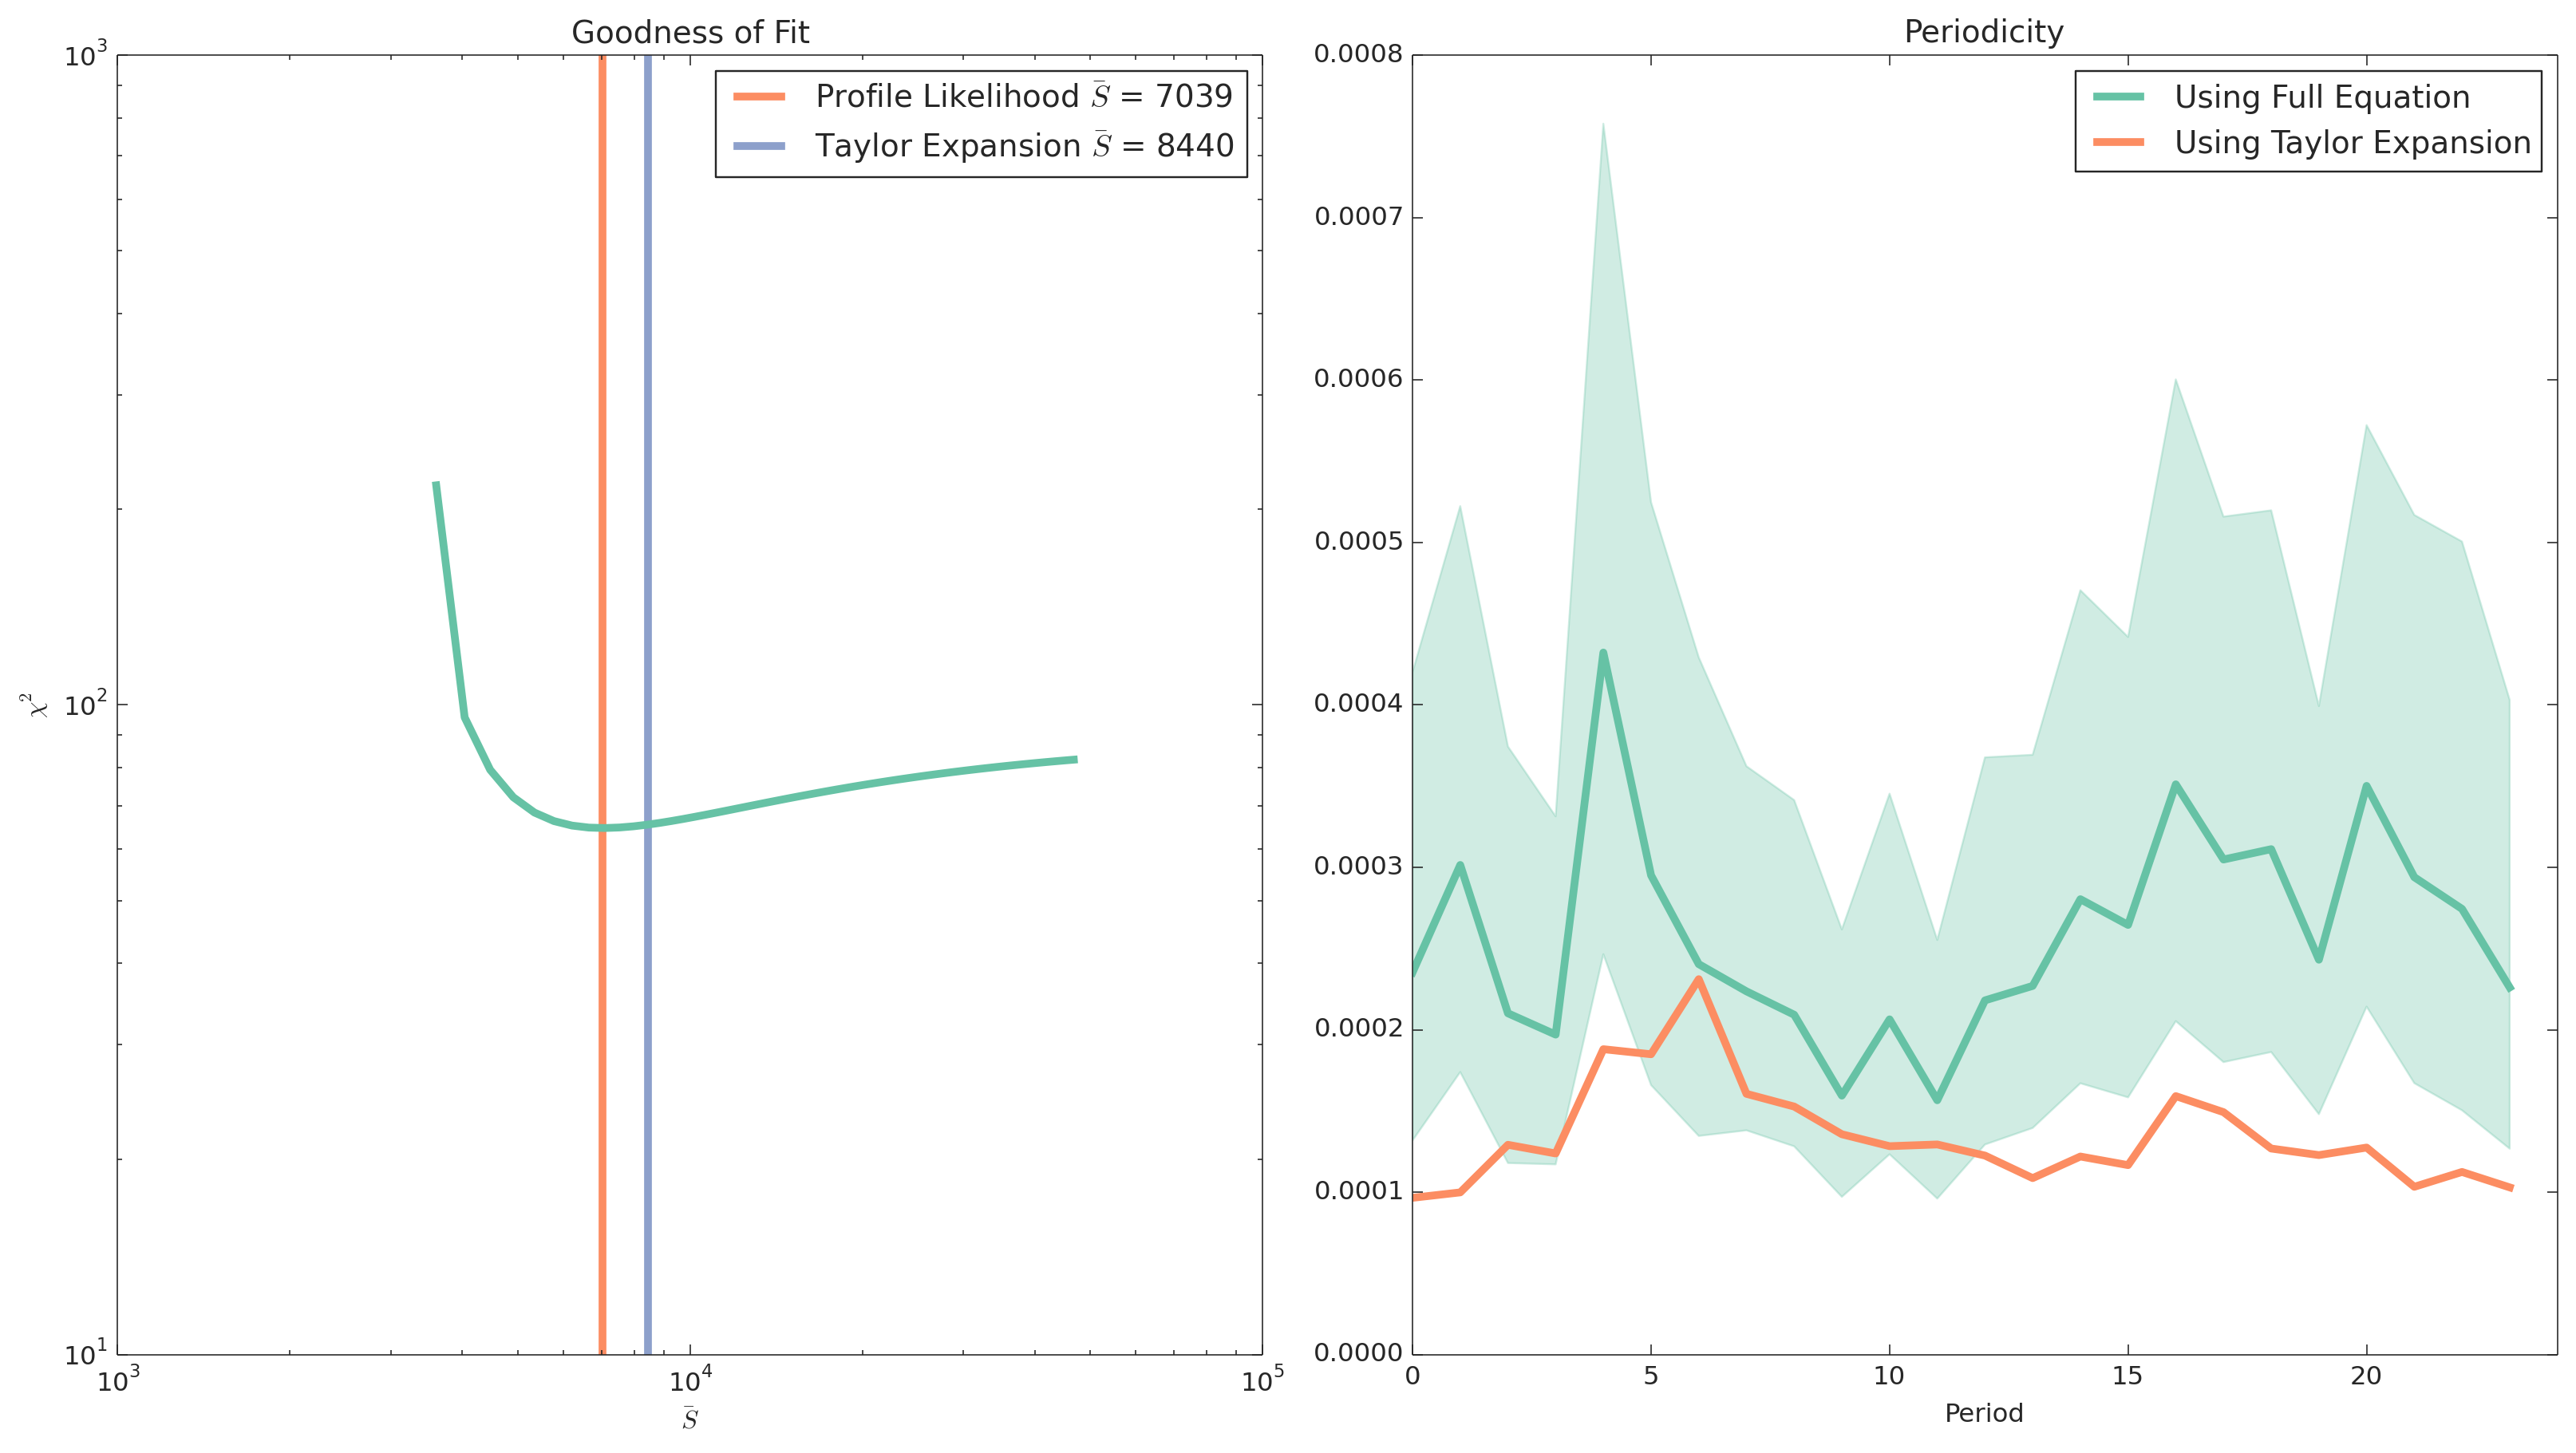
\includegraphics[max size={\textwidth}{\textheight}]{notebook_files/notebook_13_0.png}
    \par
    \end{center}
    
            \end{InvisibleVerbatim}
            
        
    
\textbf{Predictions}

Let $\tau_i^\mathrm{start}$ be the time at which epidemic $i$ begins,
and $\tau_{i}^\mathrm{end}$ the time at which the epidemic ends. We
predict using the main equation in the paper, as first presented here,
using our estimate for
$S_{\tau_i^\mathrm{start}} = \bar{S} + Z_{\tau_i^\mathrm{start}}$ as the
initial number of susceptibles, and
$I_{\tau_i^\mathrm{start}} = \rho_{\tau_i^\mathrm{start}}\,C_{\tau_i^\mathrm{start}}$
as the initial number of infected individuals for each epidemic $i$. We
then predict the dynamics of the infected and susceptible individuals
between $\tau_i^\mathrm{start}$ and $\tau_{i+1}^\mathrm{start}$.

    % Make sure that atleast 4 lines are below the HR
    \needspace{4\baselineskip}

    
        \vspace{6pt}
        \makebox[0.1\linewidth]{\smaller\hfill\tt\color{nbframe-in-prompt}In\hspace{4pt}{[}250{]}:\hspace{4pt}}\\*
        \vspace{-2.65\baselineskip}
        \begin{ColorVerbatim}
            \vspace{-0.7\baselineskip}
            \begin{Verbatim}[commandchars=\\\{\}]
\PY{c}{\PYZsh{} Initialise}
\PY{n}{predI} \PY{o}{=} \PY{n}{np}\PY{o}{.}\PY{n}{zeros\PYZus{}like}\PY{p}{(}\PY{n}{C}\PY{p}{)}
\PY{n}{predS} \PY{o}{=} \PY{n}{np}\PY{o}{.}\PY{n}{zeros\PYZus{}like}\PY{p}{(}\PY{n}{C}\PY{p}{)}

\PY{c}{\PYZsh{} Seed initial epidemic points}
\PY{k}{for} \PY{n}{e} \PY{o+ow}{in} \PY{n}{epi} \PY{p}{:}
    \PY{n}{predI}\PY{p}{[}\PY{n}{e}\PY{p}{[}\PY{l+m+mi}{0}\PY{p}{]}\PY{p}{]} \PY{o}{=} \PY{n}{rho}\PY{p}{[}\PY{n}{e}\PY{p}{[}\PY{l+m+mi}{0}\PY{p}{]}\PY{p}{]} \PY{o}{*} \PY{n}{C}\PY{p}{[}\PY{n}{e}\PY{p}{[}\PY{l+m+mi}{0}\PY{p}{]}\PY{p}{]}
    \PY{n}{predS}\PY{p}{[}\PY{n}{e}\PY{p}{[}\PY{l+m+mi}{0}\PY{p}{]}\PY{p}{]} \PY{o}{=} \PY{n}{Sbar} \PY{o}{+} \PY{n}{Z}\PY{p}{[}\PY{n}{e}\PY{p}{[}\PY{l+m+mi}{0}\PY{p}{]}\PY{p}{]}
    
    \PY{c}{\PYZsh{} Predict between epidemics}
    \PY{k}{for} \PY{n}{i} \PY{o+ow}{in} \PY{n}{e}\PY{p}{[}\PY{l+m+mi}{1}\PY{p}{:}\PY{p}{]} \PY{p}{:}
        \PY{n}{predI}\PY{p}{[}\PY{n}{i}\PY{p}{]} \PY{o}{=} \PY{n}{np}\PY{o}{.}\PY{n}{round}\PY{p}{(}\PY{n}{r}\PY{p}{[}\PY{n}{i} \PY{o}{\PYZpc{}} \PY{n}{periodicity}\PY{p}{]} \PY{o}{*} \PY{p}{(} \PY{n}{predI}\PY{p}{[}\PY{n}{i}\PY{o}{\PYZhy{}}\PY{l+m+mi}{1}\PY{p}{]} \PY{o}{*}\PY{o}{*} \PY{n}{alphaSbar} \PY{p}{)} \PY{o}{*} \PY{n}{predS}\PY{p}{[}\PY{n}{i}\PY{o}{\PYZhy{}}\PY{l+m+mi}{1}\PY{p}{]}\PY{p}{)}
        \PY{n}{predS}\PY{p}{[}\PY{n}{i}\PY{p}{]} \PY{o}{=} \PY{n}{B}\PY{p}{[}\PY{n+nb}{max}\PY{p}{(}\PY{n}{i} \PY{o}{\PYZhy{}} \PY{n}{delay}\PY{p}{,} \PY{l+m+mi}{0}\PY{p}{)}\PY{p}{]} \PY{o}{+} \PY{n}{predS}\PY{p}{[}\PY{n}{i}\PY{o}{\PYZhy{}}\PY{l+m+mi}{1}\PY{p}{]} \PY{o}{\PYZhy{}} \PY{n}{predI}\PY{p}{[}\PY{n}{i}\PY{p}{]}

    
\PY{c}{\PYZsh{} Plot   }
\PY{n}{subplot}\PY{p}{(}\PY{l+m+mi}{311}\PY{p}{)}
\PY{n}{plt}\PY{o}{.}\PY{n}{plot}\PY{p}{(}\PY{n}{C}\PY{o}{*}\PY{n}{rho}\PY{p}{,} \PY{n}{linewidth}\PY{o}{=}\PY{l+m+mi}{3}\PY{p}{)}
\PY{n}{plt}\PY{o}{.}\PY{n}{plot}\PY{p}{(}\PY{n}{predI}\PY{p}{,} \PY{n}{linewidth}\PY{o}{=}\PY{l+m+mi}{3}\PY{p}{)}
\PY{k}{for} \PY{n}{e} \PY{o+ow}{in} \PY{n}{epi}\PY{p}{[}\PY{p}{:}\PY{o}{\PYZhy{}}\PY{l+m+mi}{1}\PY{p}{]} \PY{p}{:}
    \PY{n}{axvline}\PY{p}{(}\PY{n}{e}\PY{p}{[}\PY{l+m+mi}{0}\PY{p}{]}\PY{p}{,} \PY{n}{color}\PY{o}{=}\PY{l+s}{\PYZdq{}}\PY{l+s}{r}\PY{l+s}{\PYZdq{}}\PY{p}{,} \PY{n}{linewidth}\PY{o}{=}\PY{l+m+mi}{2}\PY{p}{)}
\PY{n}{title}\PY{p}{(}\PY{l+s}{\PYZdq{}}\PY{l+s}{Per\PYZhy{}Epidemic Predictions}\PY{l+s}{\PYZdq{}}\PY{p}{)}
\PY{n}{legend}\PY{p}{(}\PY{p}{[}\PY{l+s}{\PYZdq{}}\PY{l+s}{Observed}\PY{l+s}{\PYZdq{}}\PY{p}{,} \PY{l+s}{\PYZdq{}}\PY{l+s}{Predicted}\PY{l+s}{\PYZdq{}}\PY{p}{]}\PY{p}{,} \PY{n}{loc}\PY{o}{=}\PY{l+m+mi}{2}\PY{p}{)}

\PY{n}{subplot}\PY{p}{(}\PY{l+m+mi}{312}\PY{p}{)}
\PY{n}{te} \PY{o}{=} \PY{p}{[}\PY{p}{]}
\PY{k}{for} \PY{n}{e} \PY{o+ow}{in} \PY{n}{epi} \PY{p}{:}
    \PY{n}{plt}\PY{o}{.}\PY{n}{plot}\PY{p}{(}\PY{n+nb}{range}\PY{p}{(}\PY{n+nb}{len}\PY{p}{(}\PY{n}{te}\PY{p}{)}\PY{p}{,} \PY{n+nb}{len}\PY{p}{(}\PY{n}{e}\PY{p}{)}\PY{o}{+}\PY{n+nb}{len}\PY{p}{(}\PY{n}{te}\PY{p}{)}\PY{p}{)}\PY{p}{,} \PY{n}{C}\PY{p}{[}\PY{n}{e}\PY{p}{]} \PY{o}{*} \PY{n}{rho}\PY{p}{[}\PY{n}{e}\PY{p}{]}\PY{p}{,} \PY{n}{color}\PY{o}{=}\PY{n}{colours}\PY{p}{[}\PY{l+m+mi}{0}\PY{p}{]}\PY{p}{,} \PY{n}{linewidth}\PY{o}{=}\PY{l+m+mi}{3}\PY{p}{)}
    \PY{n}{plt}\PY{o}{.}\PY{n}{plot}\PY{p}{(}\PY{n+nb}{range}\PY{p}{(}\PY{n+nb}{len}\PY{p}{(}\PY{n}{te}\PY{p}{)}\PY{p}{,} \PY{n+nb}{len}\PY{p}{(}\PY{n}{e}\PY{p}{)}\PY{o}{+}\PY{n+nb}{len}\PY{p}{(}\PY{n}{te}\PY{p}{)}\PY{p}{)}\PY{p}{,} \PY{n}{predI}\PY{p}{[}\PY{n}{e}\PY{p}{]}\PY{p}{,} \PY{n}{color}\PY{o}{=}\PY{n}{colours}\PY{p}{[}\PY{l+m+mi}{1}\PY{p}{]}\PY{p}{,} \PY{n}{linewidth}\PY{o}{=}\PY{l+m+mi}{3}\PY{p}{)}
    \PY{n}{axvline}\PY{p}{(}\PY{n+nb}{len}\PY{p}{(}\PY{n}{te}\PY{p}{)}\PY{p}{,} \PY{n}{color}\PY{o}{=}\PY{l+s}{\PYZdq{}}\PY{l+s}{r}\PY{l+s}{\PYZdq{}}\PY{p}{,} \PY{n}{linewidth}\PY{o}{=}\PY{l+m+mi}{2}\PY{p}{)}
    \PY{n}{te} \PY{o}{=} \PY{n}{np}\PY{o}{.}\PY{n}{append}\PY{p}{(}\PY{n}{te}\PY{p}{,} \PY{n+nb}{range}\PY{p}{(}\PY{n+nb}{len}\PY{p}{(}\PY{n}{e}\PY{p}{)}\PY{o}{\PYZhy{}}\PY{l+m+mi}{1}\PY{p}{)}\PY{p}{)}
\PY{n}{title}\PY{p}{(}\PY{l+s}{\PYZdq{}}\PY{l+s}{Per\PYZhy{}Epidemic Predictions with zeros removed}\PY{l+s}{\PYZdq{}}\PY{p}{)}
\PY{n}{legend}\PY{p}{(}\PY{p}{[}\PY{l+s}{\PYZdq{}}\PY{l+s}{Observed}\PY{l+s}{\PYZdq{}}\PY{p}{,} \PY{l+s}{\PYZdq{}}\PY{l+s}{Predicted}\PY{l+s}{\PYZdq{}}\PY{p}{]}\PY{p}{,} \PY{n}{loc}\PY{o}{=}\PY{l+m+mi}{2}\PY{p}{)}

\PY{n}{subplot}\PY{p}{(}\PY{l+m+mi}{313}\PY{p}{)}
\PY{n}{plt}\PY{o}{.}\PY{n}{plot}\PY{p}{(}\PY{n}{predI} \PY{o}{\PYZhy{}} \PY{n}{C}\PY{o}{*}\PY{n}{rho}\PY{p}{,} \PY{n}{linewidth}\PY{o}{=}\PY{l+m+mi}{3}\PY{p}{)}
\PY{n}{plt}\PY{o}{.}\PY{n}{axhline}\PY{p}{(}\PY{n}{np}\PY{o}{.}\PY{n}{mean}\PY{p}{(}\PY{n}{predI} \PY{o}{\PYZhy{}} \PY{n}{C} \PY{o}{*} \PY{n}{rho}\PY{p}{)}\PY{p}{,} \PY{n}{linewidth}\PY{o}{=}\PY{l+m+mi}{2}\PY{p}{)}
\PY{n}{title}\PY{p}{(}\PY{l+s}{\PYZdq{}}\PY{l+s}{Errors between actual and prediction. RMSE = }\PY{l+s}{\PYZdq{}} \PY{o}{+} \PY{n+nb}{str}\PY{p}{(}\PY{n}{np}\PY{o}{.}\PY{n}{sqrt}\PY{p}{(}\PY{n}{np}\PY{o}{.}\PY{n}{sum}\PY{p}{(}\PY{p}{(}\PY{p}{(}\PY{n}{predI} \PY{o}{\PYZhy{}} \PY{n}{C}\PY{o}{*}\PY{n}{rho}\PY{p}{)}\PY{o}{*}\PY{o}{*}\PY{l+m+mi}{2}\PY{p}{)}\PY{p}{)}\PY{o}{/}\PY{n+nb}{len}\PY{p}{(}\PY{n}{C}\PY{p}{)}\PY{p}{)}\PY{p}{)}\PY{p}{)}
\PY{n}{tight\PYZus{}layout}\PY{p}{(}\PY{p}{)}
\end{Verbatim}

            
                \vspace{-0.2\baselineskip}
            
        \end{ColorVerbatim}
    

    

        % If the first block is an image, minipage the image.  Else
        % request a certain amount of space for the input text.
        \needspace{4\baselineskip}
        
        

            % Add document contents.
            
                \begin{InvisibleVerbatim}
                \vspace{-0.5\baselineskip}
    \begin{center}
    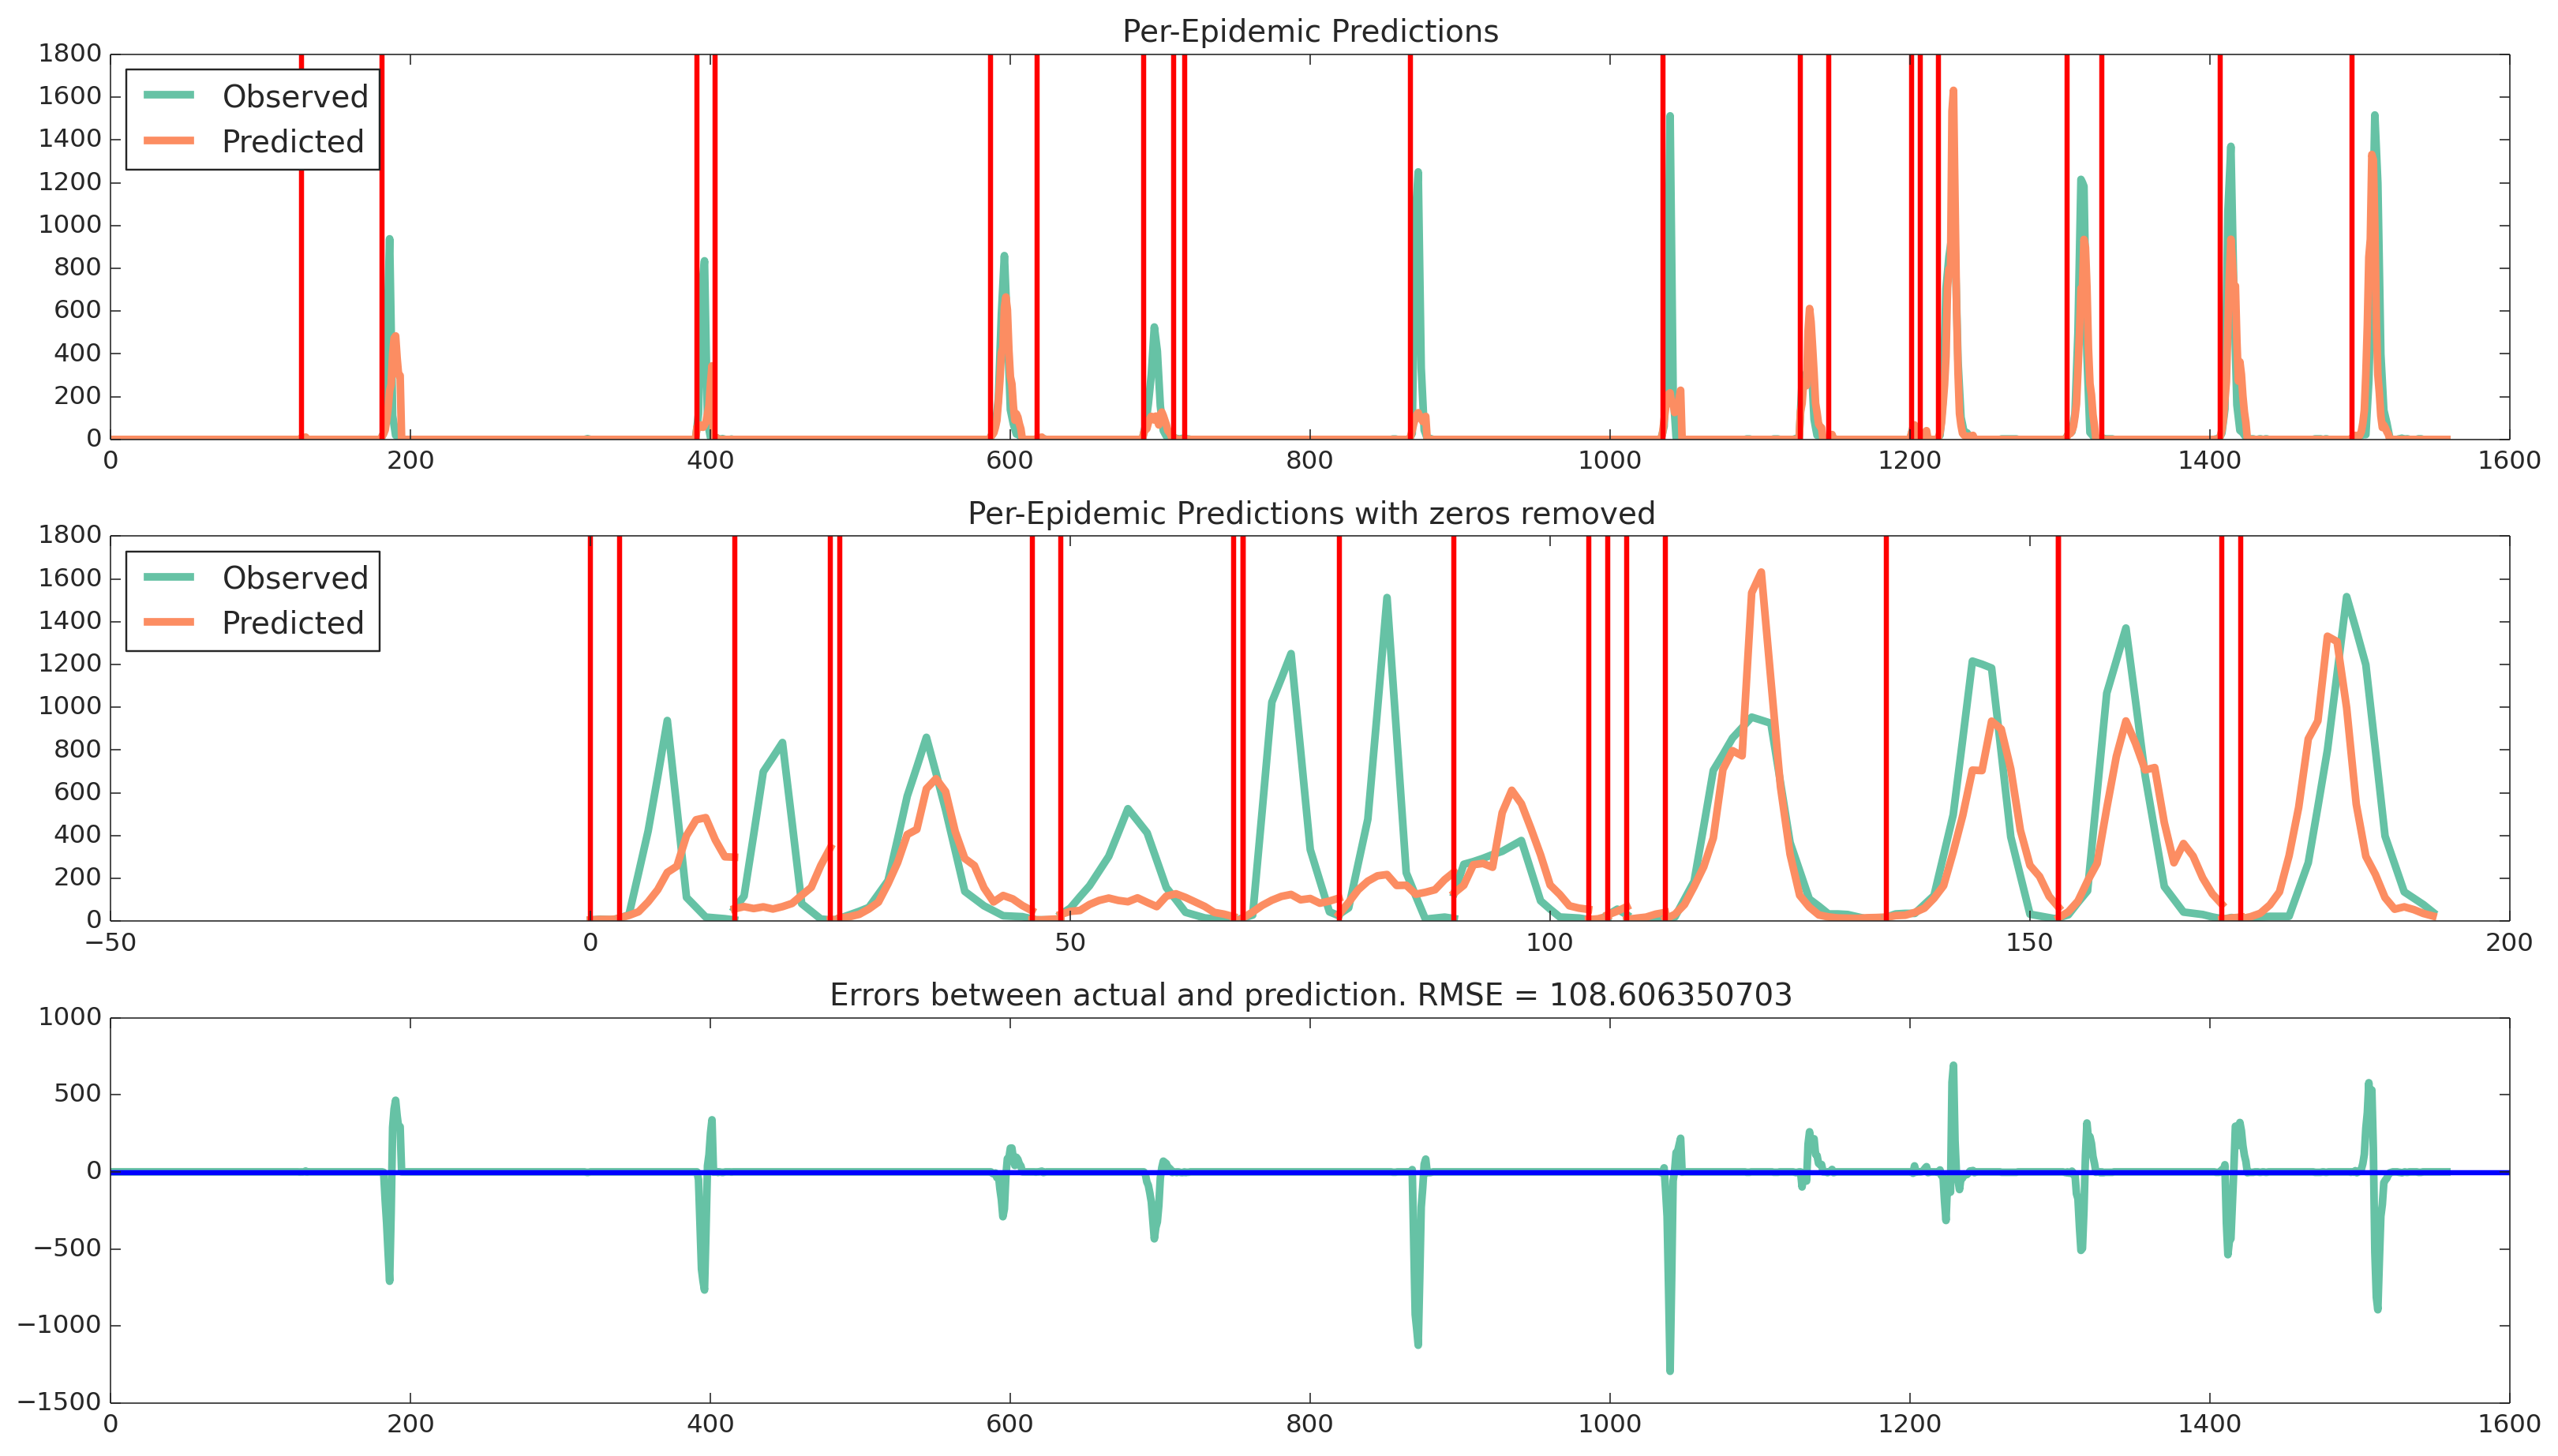
\includegraphics[max size={\textwidth}{\textheight}]{notebook_files/notebook_15_0.png}
    \par
    \end{center}
    
            \end{InvisibleVerbatim}
            
        
    
\textbf{Predicted vs Recorded Epidemic Size}

If the epidemic dynamic cannot be predicted accurately, perhaps the
final size can ? We push prediction forward until the start of the next
epidemic at time $\tau_{i+1}^\mathrm{start}$, rather than ending at
$\tau_i^\mathrm{end}$.

    % Make sure that atleast 4 lines are below the HR
    \needspace{4\baselineskip}

    
        \vspace{6pt}
        \makebox[0.1\linewidth]{\smaller\hfill\tt\color{nbframe-in-prompt}In\hspace{4pt}{[}251{]}:\hspace{4pt}}\\*
        \vspace{-2.65\baselineskip}
        \begin{ColorVerbatim}
            \vspace{-0.7\baselineskip}
            \begin{Verbatim}[commandchars=\\\{\}]
\PY{n}{pp} \PY{o}{=} \PY{n}{np}\PY{o}{.}\PY{n}{zeros}\PY{p}{(}\PY{l+m+mi}{1000}\PY{p}{)}
\PY{n}{sp} \PY{o}{=} \PY{n}{np}\PY{o}{.}\PY{n}{zeros}\PY{p}{(}\PY{l+m+mi}{1000}\PY{p}{)}
\PY{n}{pp}\PY{p}{[}\PY{l+m+mi}{0}\PY{p}{]} \PY{o}{=} \PY{n}{np}\PY{o}{.}\PY{n}{round}\PY{p}{(}\PY{n}{rho}\PY{p}{[}\PY{l+m+mi}{0}\PY{p}{]} \PY{o}{*} \PY{l+m+mi}{1}\PY{p}{)}
\PY{n}{sp}\PY{p}{[}\PY{l+m+mi}{0}\PY{p}{]} \PY{o}{=} \PY{n}{np}\PY{o}{.}\PY{n}{round}\PY{p}{(}\PY{n}{Sbar} \PY{o}{+} \PY{n}{Z}\PY{p}{[}\PY{l+m+mi}{180}\PY{p}{]}\PY{p}{)}

\PY{k}{for} \PY{n}{i} \PY{o+ow}{in} \PY{n+nb}{range}\PY{p}{(}\PY{l+m+mi}{1}\PY{p}{,} \PY{l+m+mi}{1000}\PY{p}{)} \PY{p}{:}
    \PY{n}{pp}\PY{p}{[}\PY{n}{i}\PY{p}{]} \PY{o}{=} \PY{n}{np}\PY{o}{.}\PY{n}{floor}\PY{p}{(}\PY{n}{r}\PY{p}{[}\PY{n}{i} \PY{o}{\PYZpc{}} \PY{n}{periodicity}\PY{p}{]} \PY{o}{*} \PY{p}{(} \PY{n}{pp}\PY{p}{[}\PY{n}{i}\PY{o}{\PYZhy{}}\PY{l+m+mi}{1}\PY{p}{]} \PY{o}{*}\PY{o}{*} \PY{n}{alphaSbar} \PY{p}{)} \PY{o}{*} \PY{n}{sp}\PY{p}{[}\PY{n}{i}\PY{o}{\PYZhy{}}\PY{l+m+mi}{1}\PY{p}{]}\PY{p}{)}
    \PY{n}{sp}\PY{p}{[}\PY{n}{i}\PY{p}{]} \PY{o}{=} \PY{n}{np}\PY{o}{.}\PY{n}{floor}\PY{p}{(}\PY{n}{B}\PY{p}{[}\PY{n}{i}\PY{p}{]} \PY{o}{+} \PY{n}{sp}\PY{p}{[}\PY{n}{i}\PY{o}{\PYZhy{}}\PY{l+m+mi}{1}\PY{p}{]} \PY{o}{\PYZhy{}} \PY{n}{pp}\PY{p}{[}\PY{n}{i}\PY{p}{]}\PY{p}{)}
    
\PY{n}{plt}\PY{o}{.}\PY{n}{plot}\PY{p}{(}\PY{n}{pp}\PY{p}{,} \PY{n}{linewidth}\PY{o}{=}\PY{l+m+mi}{3}\PY{p}{)}
\end{Verbatim}

            
                \vspace{-0.2\baselineskip}
            
        \end{ColorVerbatim}
    

    

        % If the first block is an image, minipage the image.  Else
        % request a certain amount of space for the input text.
        \needspace{4\baselineskip}
        
        

            % Add document contents.
            
                \makebox[0.1\linewidth]{\smaller\hfill\tt\color{nbframe-out-prompt}Out\hspace{4pt}{[}251{]}:\hspace{4pt}}\\*
                \vspace{-2.55\baselineskip}\begin{InvisibleVerbatim}
                \vspace{-0.5\baselineskip}
\begin{alltt}[<matplotlib.lines.Line2D at 0x134d87710>]\end{alltt}

            \end{InvisibleVerbatim}
            
                \begin{InvisibleVerbatim}
                \vspace{-0.5\baselineskip}
    \begin{center}
    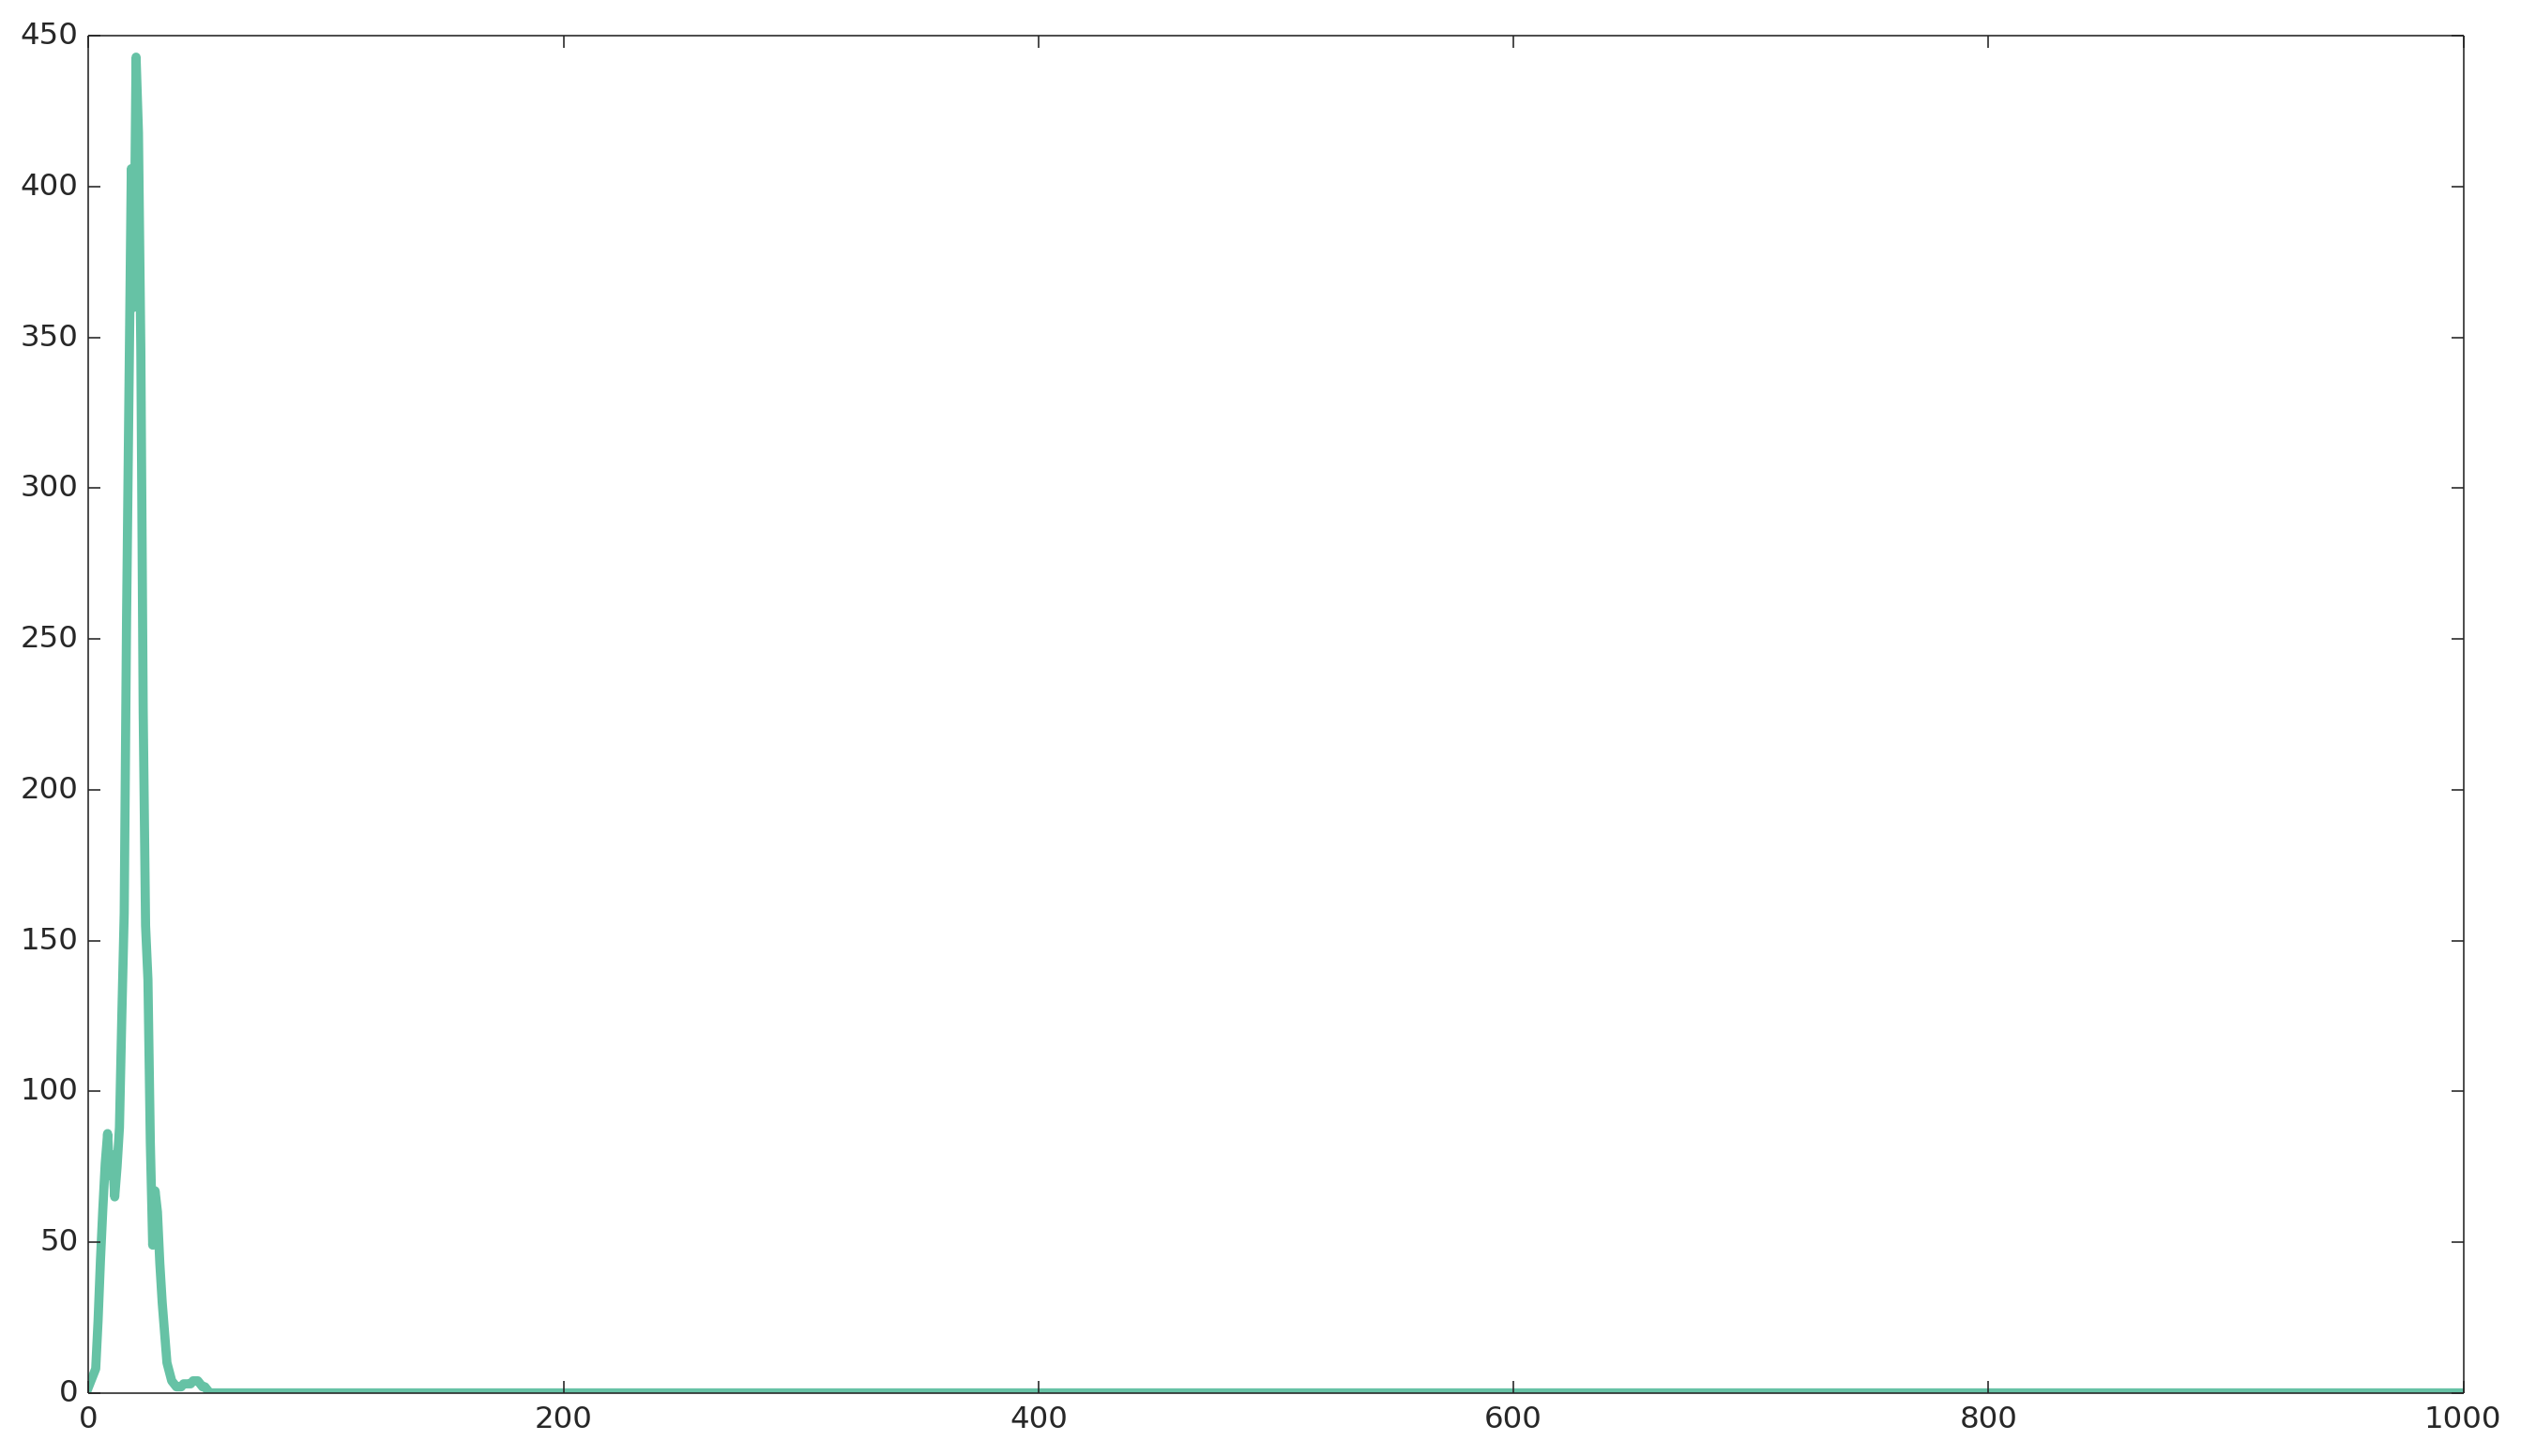
\includegraphics[max size={\textwidth}{\textheight}]{notebook_files/notebook_17_1.png}
    \par
    \end{center}
    
            \end{InvisibleVerbatim}
            
        
    


    % Make sure that atleast 4 lines are below the HR
    \needspace{4\baselineskip}

    
        \vspace{6pt}
        \makebox[0.1\linewidth]{\smaller\hfill\tt\color{nbframe-in-prompt}In\hspace{4pt}{[}253{]}:\hspace{4pt}}\\*
        \vspace{-2.65\baselineskip}
        \begin{ColorVerbatim}
            \vspace{-0.7\baselineskip}
            \begin{Verbatim}[commandchars=\\\{\}]
\PY{c}{\PYZsh{} Find epidemic start times}
\PY{n}{starts} \PY{o}{=} \PY{p}{[}\PY{n}{e}\PY{p}{[}\PY{l+m+mi}{0}\PY{p}{]} \PY{k}{for} \PY{n}{e} \PY{o+ow}{in} \PY{n}{epi}\PY{p}{]}
\PY{n}{starts}\PY{o}{.}\PY{n}{append}\PY{p}{(}\PY{n+nb}{len}\PY{p}{(}\PY{n}{rho}\PY{p}{)}\PY{p}{)} \PY{c}{\PYZsh{} add final time}
\PY{n}{prI} \PY{o}{=} \PY{p}{[}\PY{p}{]}

\PY{c}{\PYZsh{} For each epidemic, predict until the time of the next epidemic}
\PY{k}{for} \PY{n}{i}\PY{p}{,} \PY{n}{time} \PY{o+ow}{in} \PY{n+nb}{enumerate}\PY{p}{(}\PY{n}{starts}\PY{p}{[}\PY{p}{:}\PY{o}{\PYZhy{}}\PY{l+m+mi}{1}\PY{p}{]}\PY{p}{)} \PY{p}{:}
    \PY{c}{\PYZsh{} Seed the epidemic}
    \PY{n}{predI2} \PY{o}{=} \PY{n}{np}\PY{o}{.}\PY{n}{zeros}\PY{p}{(}\PY{n}{starts}\PY{p}{[}\PY{n}{i}\PY{o}{+}\PY{l+m+mi}{1}\PY{p}{]} \PY{o}{\PYZhy{}} \PY{n}{time}\PY{p}{)}
    \PY{n}{predS2} \PY{o}{=} \PY{n}{np}\PY{o}{.}\PY{n}{zeros}\PY{p}{(}\PY{n}{starts}\PY{p}{[}\PY{n}{i}\PY{o}{+}\PY{l+m+mi}{1}\PY{p}{]} \PY{o}{\PYZhy{}} \PY{n}{time}\PY{p}{)}
    \PY{n}{predI2}\PY{p}{[}\PY{l+m+mi}{0}\PY{p}{]} \PY{o}{=} \PY{n}{np}\PY{o}{.}\PY{n}{round}\PY{p}{(}\PY{n}{rho}\PY{p}{[}\PY{n}{time}\PY{p}{]} \PY{o}{*} \PY{n}{C}\PY{p}{[}\PY{n}{time}\PY{p}{]}\PY{p}{)}
    \PY{n}{predS2}\PY{p}{[}\PY{l+m+mi}{0}\PY{p}{]} \PY{o}{=} \PY{n}{np}\PY{o}{.}\PY{n}{round}\PY{p}{(}\PY{n}{Sbar} \PY{o}{+} \PY{n}{Z}\PY{p}{[}\PY{n}{time}\PY{p}{]}\PY{p}{)}
    
    \PY{c}{\PYZsh{} Predict between epidemics}
    \PY{k}{for} \PY{n}{j} \PY{o+ow}{in} \PY{n+nb}{range}\PY{p}{(}\PY{l+m+mi}{1}\PY{p}{,} \PY{n+nb}{len}\PY{p}{(}\PY{n}{predI2}\PY{p}{)}\PY{p}{)} \PY{p}{:}
        \PY{n}{predI2}\PY{p}{[}\PY{n}{j}\PY{p}{]} \PY{o}{=} \PY{n}{np}\PY{o}{.}\PY{n}{round}\PY{p}{(}\PY{n}{r}\PY{p}{[}\PY{p}{(}\PY{n}{time} \PY{o}{+} \PY{n}{j}\PY{p}{)} \PY{o}{\PYZpc{}} \PY{n}{periodicity}\PY{p}{]} \PY{o}{*} \PY{p}{(} \PY{n}{predI2}\PY{p}{[}\PY{n}{j}\PY{o}{\PYZhy{}}\PY{l+m+mi}{1}\PY{p}{]} \PY{o}{*}\PY{o}{*} \PY{n}{alphaSbar} \PY{p}{)} \PY{o}{*} \PY{n}{predS2}\PY{p}{[}\PY{n}{j}\PY{o}{\PYZhy{}}\PY{l+m+mi}{1}\PY{p}{]}\PY{p}{)}
        \PY{n}{predS2}\PY{p}{[}\PY{n}{j}\PY{p}{]} \PY{o}{=} \PY{n}{np}\PY{o}{.}\PY{n}{round}\PY{p}{(}\PY{n}{B}\PY{p}{[}\PY{n+nb}{max}\PY{p}{(}\PY{n}{j} \PY{o}{\PYZhy{}} \PY{n}{delay}\PY{p}{,} \PY{l+m+mi}{0}\PY{p}{)}\PY{p}{]} \PY{o}{+} \PY{n}{predS2}\PY{p}{[}\PY{n}{j}\PY{o}{\PYZhy{}}\PY{l+m+mi}{1}\PY{p}{]} \PY{o}{\PYZhy{}} \PY{n}{predI2}\PY{p}{[}\PY{n}{j}\PY{p}{]}\PY{p}{)}
        
    \PY{c}{\PYZsh{} When the prediction dips below sensitivity, assume the epidemic is extinct}
    \PY{k}{if} \PY{n}{size}\PY{p}{(}\PY{n}{np}\PY{o}{.}\PY{n}{where}\PY{p}{(}\PY{n}{predI2} \PY{o}{\PYZlt{}} \PY{n}{sensitivity}\PY{p}{)}\PY{p}{[}\PY{l+m+mi}{0}\PY{p}{]}\PY{p}{)} \PY{p}{:}
        \PY{n}{predI2}\PY{p}{[}\PY{p}{(}\PY{n}{np}\PY{o}{.}\PY{n}{where}\PY{p}{(}\PY{n}{predI2} \PY{o}{\PYZlt{}} \PY{n}{sensitivity}\PY{p}{)}\PY{p}{[}\PY{l+m+mi}{0}\PY{p}{]}\PY{p}{[}\PY{l+m+mi}{0}\PY{p}{]}\PY{p}{)}\PY{p}{:}\PY{p}{]} \PY{o}{=} \PY{l+m+mi}{0}
    
    \PY{c}{\PYZsh{} Save result}
    \PY{n}{prI}\PY{o}{.}\PY{n}{append}\PY{p}{(}\PY{n}{predI2}\PY{p}{)}
    
    
\PY{c}{\PYZsh{} Calculate epidemic sizes, both predicted and actual}
\PY{n}{actualsizes} \PY{o}{=} \PY{n}{np}\PY{o}{.}\PY{n}{array}\PY{p}{(}\PY{p}{[}\PY{n}{np}\PY{o}{.}\PY{n}{sum}\PY{p}{(}\PY{n}{C}\PY{p}{[}\PY{n}{e}\PY{p}{]} \PY{o}{*} \PY{n}{rho}\PY{p}{[}\PY{n}{e}\PY{p}{]}\PY{p}{)} \PY{k}{for} \PY{n}{e} \PY{o+ow}{in} \PY{n}{epi}\PY{p}{]}\PY{p}{)}\PY{o}{.}\PY{n}{reshape}\PY{p}{(}\PY{n+nb}{len}\PY{p}{(}\PY{n}{epi}\PY{p}{)}\PY{p}{,}\PY{l+m+mi}{1}\PY{p}{)}
\PY{n}{predictedsizes} \PY{o}{=} \PY{p}{[}\PY{n}{np}\PY{o}{.}\PY{n}{sum}\PY{p}{(}\PY{n}{pred}\PY{p}{)} \PY{k}{for} \PY{n}{pred} \PY{o+ow}{in} \PY{n}{prI}\PY{p}{]}

\PY{c}{\PYZsh{} Line of best fit and R\PYZca{}2}
\PY{n}{sizeline} \PY{o}{=} \PY{n}{linear\PYZus{}model}\PY{o}{.}\PY{n}{BayesianRidge}\PY{p}{(}\PY{n}{compute\PYZus{}score}\PY{o}{=}\PY{n+nb+bp}{True}\PY{p}{,} \PY{n}{fit\PYZus{}intercept}\PY{o}{=}\PY{n+nb+bp}{True}\PY{p}{)}
\PY{n}{sizeline}\PY{o}{.}\PY{n}{fit}\PY{p}{(}\PY{n}{actualsizes}\PY{o}{.}\PY{n}{reshape}\PY{p}{(}\PY{n+nb}{len}\PY{p}{(}\PY{n}{actualsizes}\PY{p}{)}\PY{p}{,}\PY{l+m+mi}{1}\PY{p}{)}\PY{p}{,} \PY{n}{predictedsizes}\PY{p}{)}


\PY{c}{\PYZsh{} Plot}
\PY{n}{subplot}\PY{p}{(}\PY{l+m+mi}{211}\PY{p}{)}
\PY{n}{plt}\PY{o}{.}\PY{n}{plot}\PY{p}{(}\PY{n}{C}\PY{o}{*}\PY{n}{rho}\PY{p}{,} \PY{n}{linewidth}\PY{o}{=}\PY{l+m+mi}{3}\PY{p}{)}
\PY{k}{for} \PY{n}{i}\PY{p}{,} \PY{n}{e} \PY{o+ow}{in} \PY{n+nb}{enumerate}\PY{p}{(}\PY{n}{epi}\PY{p}{)} \PY{p}{:}
    \PY{n}{plt}\PY{o}{.}\PY{n}{plot}\PY{p}{(}\PY{n+nb}{range}\PY{p}{(}\PY{n}{e}\PY{p}{[}\PY{l+m+mi}{0}\PY{p}{]}\PY{p}{,} \PY{n}{e}\PY{p}{[}\PY{l+m+mi}{0}\PY{p}{]} \PY{o}{+} \PY{n+nb}{len}\PY{p}{(}\PY{n}{prI}\PY{p}{[}\PY{n}{i}\PY{p}{]}\PY{p}{)}\PY{p}{)} \PY{p}{,} \PY{n}{prI}\PY{p}{[}\PY{n}{i}\PY{p}{]}\PY{p}{,} \PY{n}{color}\PY{o}{=}\PY{n}{colours}\PY{p}{[}\PY{l+m+mi}{1}\PY{p}{]}\PY{p}{,} \PY{n}{linewidth}\PY{o}{=}\PY{l+m+mi}{3}\PY{p}{)}
\PY{c}{\PYZsh{}    axvline(len(te), color=\PYZdq{}r\PYZdq{}, linewidth=2)}
\PY{c}{\PYZsh{}    te = np.append(te, range(len(e)\PYZhy{}1))}
\PY{n}{title}\PY{p}{(}\PY{l+s}{\PYZdq{}}\PY{l+s}{Per\PYZhy{}Epidemic Long Predictions}\PY{l+s}{\PYZdq{}}\PY{p}{)}
\PY{n}{legend}\PY{p}{(}\PY{p}{[}\PY{l+s}{\PYZdq{}}\PY{l+s}{Observed}\PY{l+s}{\PYZdq{}}\PY{p}{,} \PY{l+s}{\PYZdq{}}\PY{l+s}{Predicted}\PY{l+s}{\PYZdq{}}\PY{p}{]}\PY{p}{,} \PY{n}{loc}\PY{o}{=}\PY{l+m+mi}{2}\PY{p}{)}



\PY{n}{subplot}\PY{p}{(}\PY{l+m+mi}{212}\PY{p}{)}
\PY{n}{plt}\PY{o}{.}\PY{n}{scatter}\PY{p}{(}\PY{n}{actualsizes}\PY{p}{,} \PY{n}{predictedsizes}\PY{p}{,} \PY{n}{s}\PY{o}{=}\PY{l+m+mi}{20}\PY{o}{*}\PY{n}{np}\PY{o}{.}\PY{n}{array}\PY{p}{(}\PY{n+nb}{range}\PY{p}{(}\PY{n+nb}{len}\PY{p}{(}\PY{n}{actualsizes}\PY{p}{)}\PY{p}{)}\PY{p}{)}\PY{p}{,} \PY{n}{c}\PY{o}{=}\PY{p}{(}\PY{n}{t}\PY{p}{[}\PY{n}{starts}\PY{p}{[}\PY{p}{:}\PY{o}{\PYZhy{}}\PY{l+m+mi}{1}\PY{p}{]}\PY{p}{]} \PY{o}{\PYZpc{}} \PY{n}{periodicity}\PY{p}{)}\PY{p}{)}
\PY{n}{plt}\PY{o}{.}\PY{n}{plot}\PY{p}{(}\PY{n}{actualsizes}\PY{p}{,} \PY{n}{sizeline}\PY{o}{.}\PY{n}{predict}\PY{p}{(}\PY{n}{actualsizes}\PY{p}{)}\PY{p}{,} \PY{n}{linewidth}\PY{o}{=}\PY{l+m+mi}{3}\PY{p}{)}
\PY{n}{plt}\PY{o}{.}\PY{n}{gray}\PY{p}{(}\PY{p}{)}
\PY{n}{title}\PY{p}{(}\PY{l+s}{\PYZdq{}}\PY{l+s}{Predicted vs Actual Epidemic Sizes. Lighter = Later in Year; Bigger = Later in Time}\PY{l+s}{\PYZdq{}}\PY{p}{)}
\PY{n}{xlabel}\PY{p}{(}\PY{l+s}{\PYZdq{}}\PY{l+s}{Actual Size}\PY{l+s}{\PYZdq{}}\PY{p}{)}
\PY{n}{ylabel}\PY{p}{(}\PY{l+s}{\PYZdq{}}\PY{l+s}{Predicted Size}\PY{l+s}{\PYZdq{}}\PY{p}{)}
\PY{n}{legend}\PY{p}{(}\PY{p}{[}\PY{l+s}{r\PYZdq{}}\PY{l+s}{R\PYZdl{}\PYZca{}2\PYZdl{} = }\PY{l+s}{\PYZdq{}} \PY{o}{+} \PY{n+nb}{str}\PY{p}{(}\PY{n}{sizeline}\PY{o}{.}\PY{n}{score}\PY{p}{(}\PY{n}{actualsizes}\PY{o}{.}\PY{n}{reshape}\PY{p}{(}\PY{n+nb}{len}\PY{p}{(}\PY{n}{actualsizes}\PY{p}{)}\PY{p}{,}\PY{l+m+mi}{1}\PY{p}{)}\PY{p}{,} \PY{n}{predictedsizes}\PY{p}{)}\PY{p}{)}\PY{p}{]}\PY{p}{,} \PY{n}{loc}\PY{o}{=}\PY{l+m+mi}{0}\PY{p}{)}
\PY{n}{xlim}\PY{p}{(}\PY{p}{[}\PY{l+m+mi}{0}\PY{p}{,} \PY{l+m+mf}{1.05}\PY{o}{*}\PY{n}{np}\PY{o}{.}\PY{n}{max}\PY{p}{(}\PY{n}{actualsizes}\PY{p}{)}\PY{p}{]}\PY{p}{)}

\PY{n}{tight\PYZus{}layout}\PY{p}{(}\PY{p}{)}
\end{Verbatim}

            
                \vspace{-0.2\baselineskip}
            
        \end{ColorVerbatim}
    

    

        % If the first block is an image, minipage the image.  Else
        % request a certain amount of space for the input text.
        \needspace{4\baselineskip}
        
        

            % Add document contents.
            
                \begin{InvisibleVerbatim}
                \vspace{-0.5\baselineskip}
    \begin{center}
    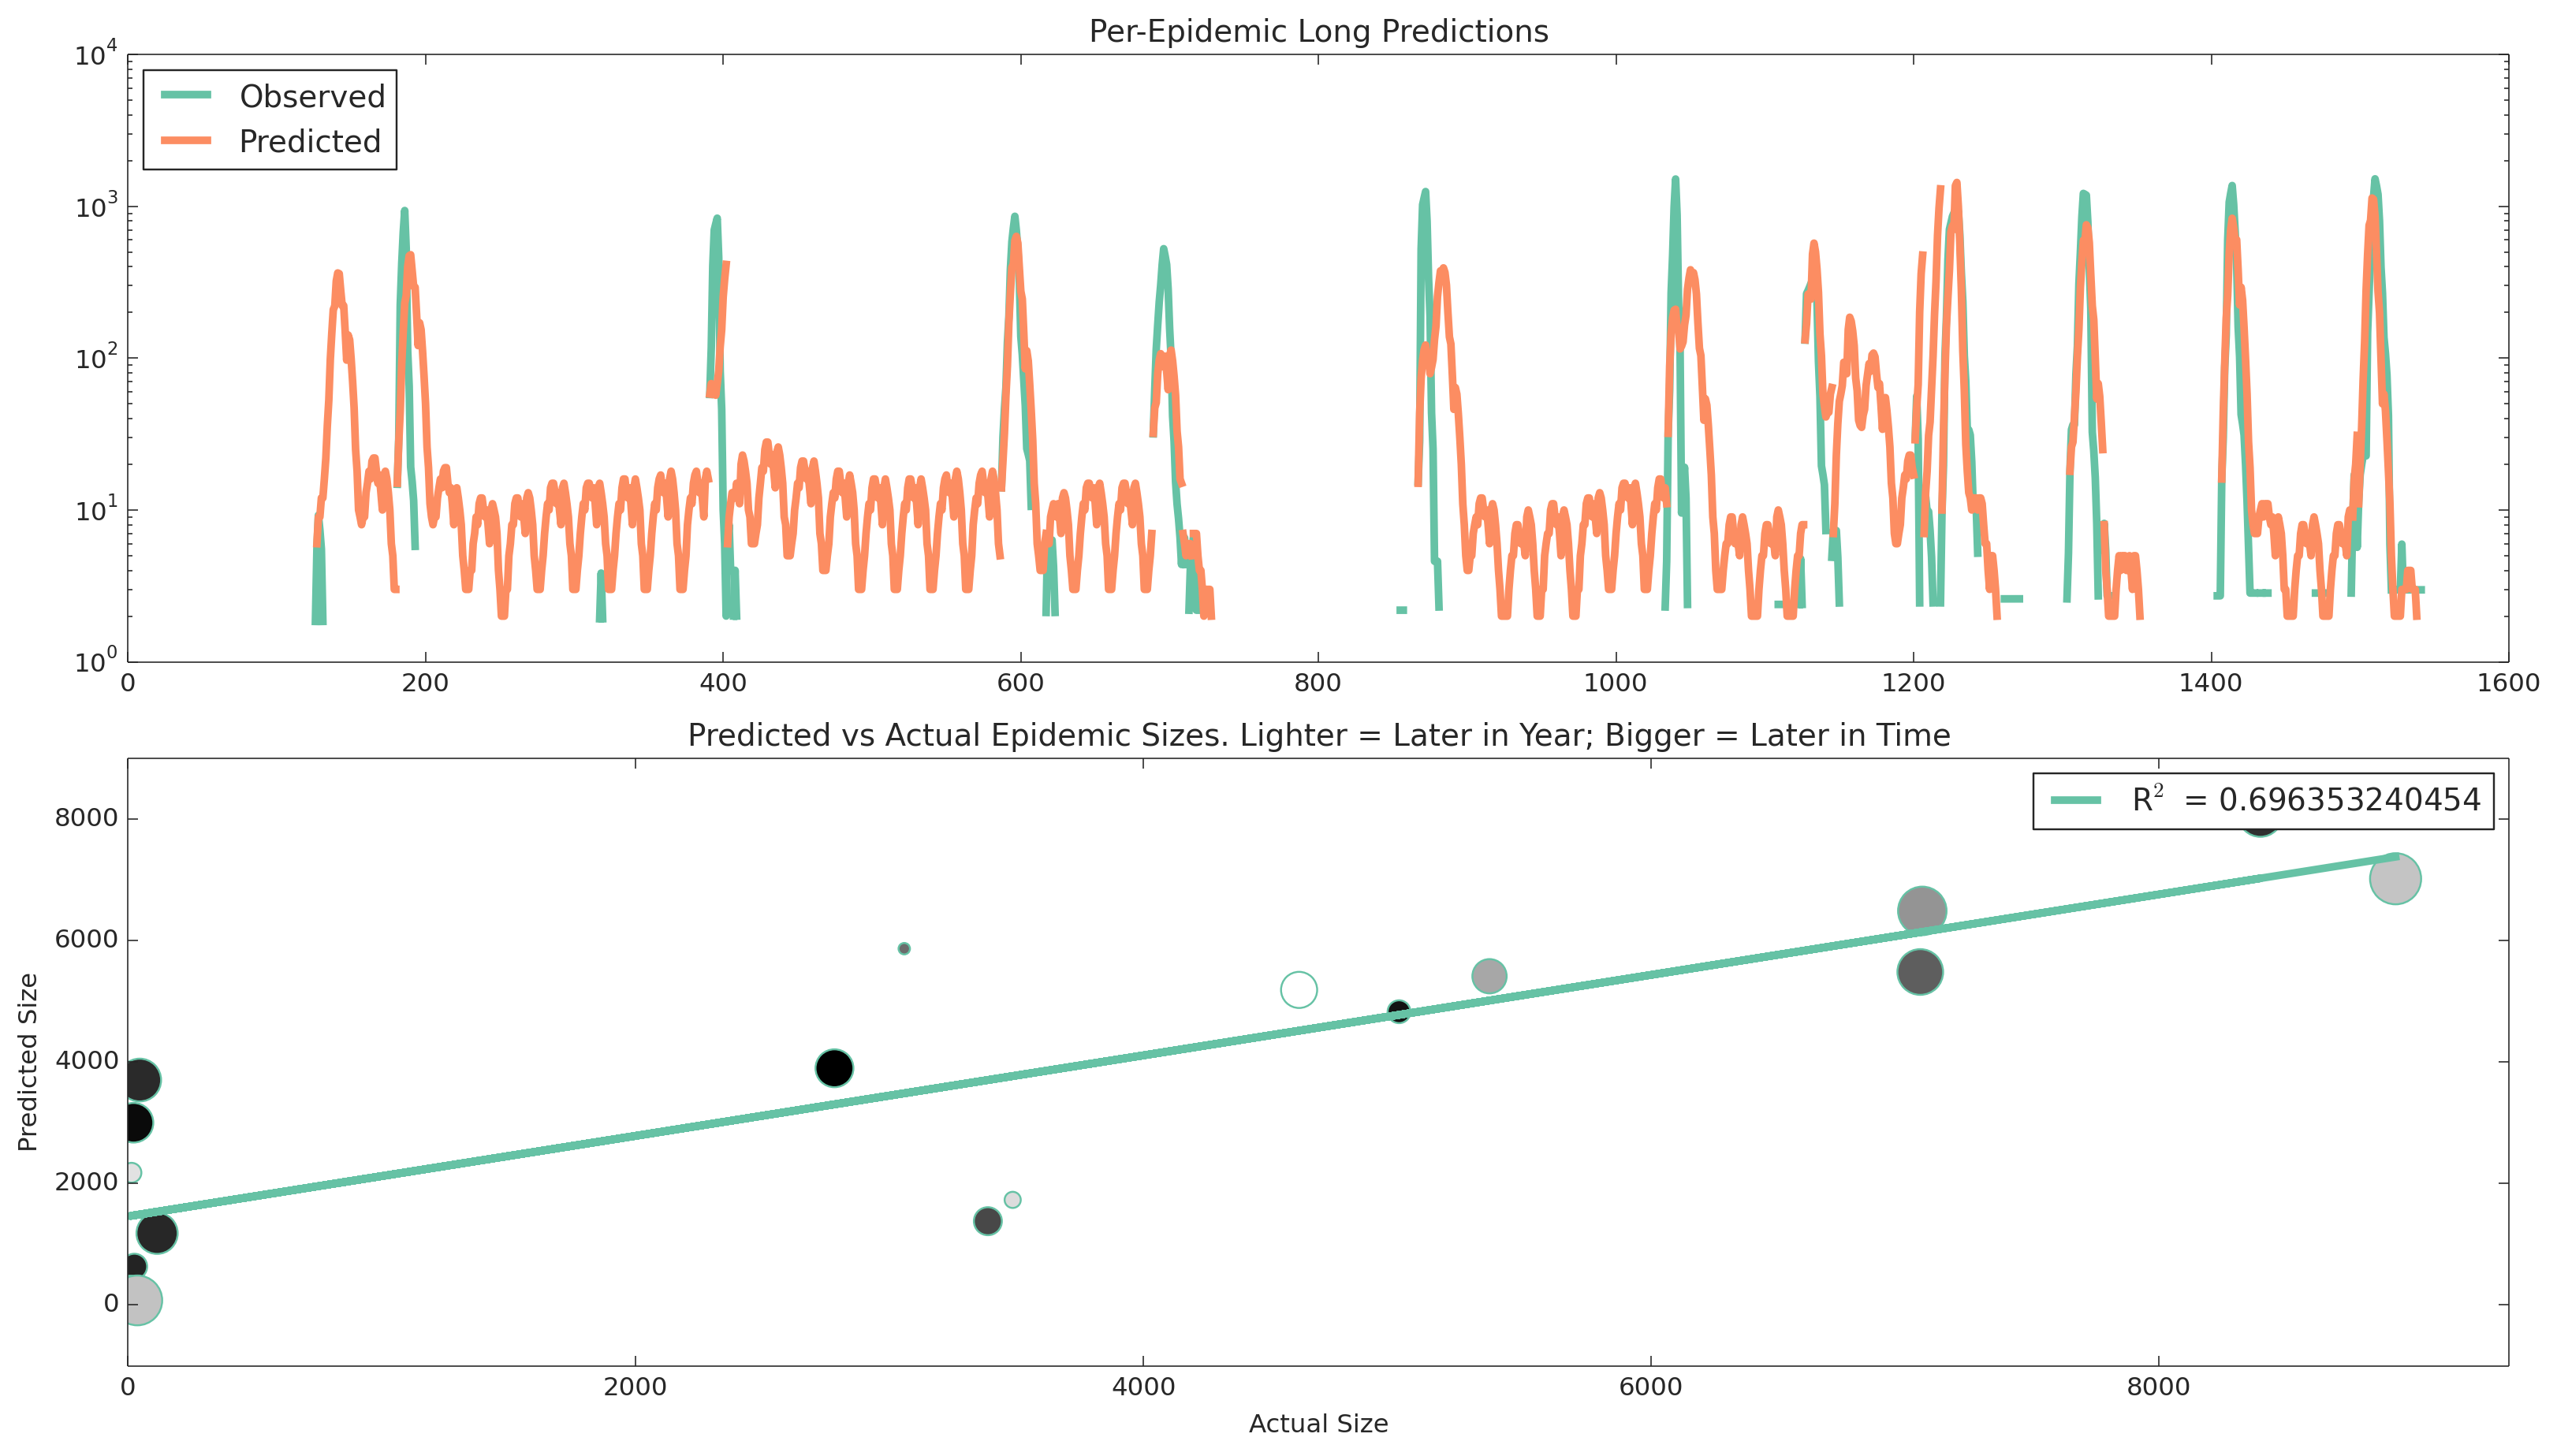
\includegraphics[max size={\textwidth}{\textheight}]{notebook_files/notebook_18_0.png}
    \par
    \end{center}
    
            \end{InvisibleVerbatim}
            
        
    
\textbf{Fraction Infected per Epidemic}

The fraction of the total susceptibles that get infected during an
epidemic can be used as a diagnostic tool against certain numerical
issues. This quantity should be between zero and one, and is defined for
epidemic $i$ as :

\[
F_i = \frac{\displaystyle\int\limits_{\tau_i^\mathrm{start}}^{\tau_i^\mathrm{end}} I_t \,\mathrm{d}t}{\displaystyle S_{\tau_i} + \int\limits_{\tau_i^\mathrm{start}}^{\tau_{i}^\mathrm{end}} B_t \,\mathrm{d}t}.
\]

The numerator here is the total number of infected individuals during
the epidemic, and the denominator is the number of susceptibles at the
beginning of the epidemic, plus the number of births that occur during
the period of the epidemic.

Near-zeros may indicate spurious infections that do not lead to ``real''
epidemics. This may or may not imply that the sensitivity threshold may
be too low.

    % Make sure that atleast 4 lines are below the HR
    \needspace{4\baselineskip}

    
        \vspace{6pt}
        \makebox[0.1\linewidth]{\smaller\hfill\tt\color{nbframe-in-prompt}In\hspace{4pt}{[}254{]}:\hspace{4pt}}\\*
        \vspace{-2.65\baselineskip}
        \begin{ColorVerbatim}
            \vspace{-0.7\baselineskip}
            \begin{Verbatim}[commandchars=\\\{\}]
\PY{c}{\PYZsh{} Calculate F for each epidemic}
\PY{n}{F} \PY{o}{=} \PY{p}{[}\PY{n}{np}\PY{o}{.}\PY{n}{sum}\PY{p}{(}\PY{n}{predI}\PY{p}{[}\PY{n}{e}\PY{p}{]}\PY{p}{)} \PY{o}{/} \PY{p}{(}\PY{n}{Sbar} \PY{o}{+} \PY{n}{Z}\PY{p}{[}\PY{n}{e}\PY{p}{[}\PY{l+m+mi}{0}\PY{p}{]}\PY{p}{]} \PY{o}{+} \PY{n}{np}\PY{o}{.}\PY{n}{sum}\PY{p}{(}\PY{n}{B}\PY{p}{[}\PY{n}{e}\PY{p}{]}\PY{p}{)}\PY{p}{)}\PY{o}{.}\PY{n}{astype}\PY{p}{(}\PY{n+nb}{float}\PY{p}{)} \PY{k}{for} \PY{n}{e} \PY{o+ow}{in} \PY{n}{epi}\PY{p}{]}

\PY{c}{\PYZsh{} Plot}
\PY{n}{plt}\PY{o}{.}\PY{n}{plot}\PY{p}{(}\PY{n}{F}\PY{p}{,} \PY{n}{linewidth}\PY{o}{=}\PY{l+m+mi}{3}\PY{p}{)}
\PY{n}{title}\PY{p}{(}\PY{l+s}{r\PYZdq{}}\PY{l+s}{Fraction \PYZdl{}F\PYZus{}i\PYZdl{} of Susceptibles Infected per Epidemic}\PY{l+s}{\PYZdq{}}\PY{p}{)}
\PY{n}{xlabel}\PY{p}{(}\PY{l+s}{\PYZdq{}}\PY{l+s}{Epidemic}\PY{l+s}{\PYZdq{}}\PY{p}{)}

\PY{c}{\PYZsh{} For the SIR, we can calculate the true value of F by using actual S, and not the reconstruction :}
\PY{k}{if} \PY{o+ow}{not} \PY{p}{(}\PY{n}{LONDON} \PY{o+ow}{or} \PY{n}{ICELAND} \PY{o+ow}{or} \PY{n}{FAROE} \PY{o+ow}{or} \PY{n}{BORNHOLM}\PY{p}{)} \PY{p}{:}
    \PY{n}{F2} \PY{o}{=} \PY{p}{[}\PY{n}{np}\PY{o}{.}\PY{n}{sum}\PY{p}{(}\PY{n}{predI}\PY{p}{[}\PY{n}{e}\PY{p}{]}\PY{p}{)} \PY{o}{/} \PY{p}{(}\PY{n}{S}\PY{p}{[}\PY{n}{e}\PY{p}{[}\PY{l+m+mi}{0}\PY{p}{]}\PY{p}{]} \PY{o}{+} \PY{n}{np}\PY{o}{.}\PY{n}{sum}\PY{p}{(}\PY{n}{B}\PY{p}{[}\PY{n}{e}\PY{p}{]}\PY{p}{)}\PY{p}{)}\PY{o}{.}\PY{n}{astype}\PY{p}{(}\PY{n+nb}{float}\PY{p}{)} \PY{k}{for} \PY{n}{e} \PY{o+ow}{in} \PY{n}{epi}\PY{p}{]}
    \PY{n}{plt}\PY{o}{.}\PY{n}{plot}\PY{p}{(}\PY{n}{F2}\PY{p}{,} \PY{n}{linewidth}\PY{o}{=}\PY{l+m+mi}{3}\PY{p}{)}
    \PY{n}{legend}\PY{p}{(}\PY{p}{[}\PY{l+s}{\PYZdq{}}\PY{l+s}{Using Predicted Susceptibles}\PY{l+s}{\PYZdq{}}\PY{p}{,} \PY{l+s}{\PYZdq{}}\PY{l+s}{Using Real Susceptibles}\PY{l+s}{\PYZdq{}}\PY{p}{]}\PY{p}{)}
\end{Verbatim}

            
                \vspace{-0.2\baselineskip}
            
        \end{ColorVerbatim}
    

    

        % If the first block is an image, minipage the image.  Else
        % request a certain amount of space for the input text.
        \needspace{4\baselineskip}
        
        

            % Add document contents.
            
                \begin{InvisibleVerbatim}
                \vspace{-0.5\baselineskip}
    \begin{center}
    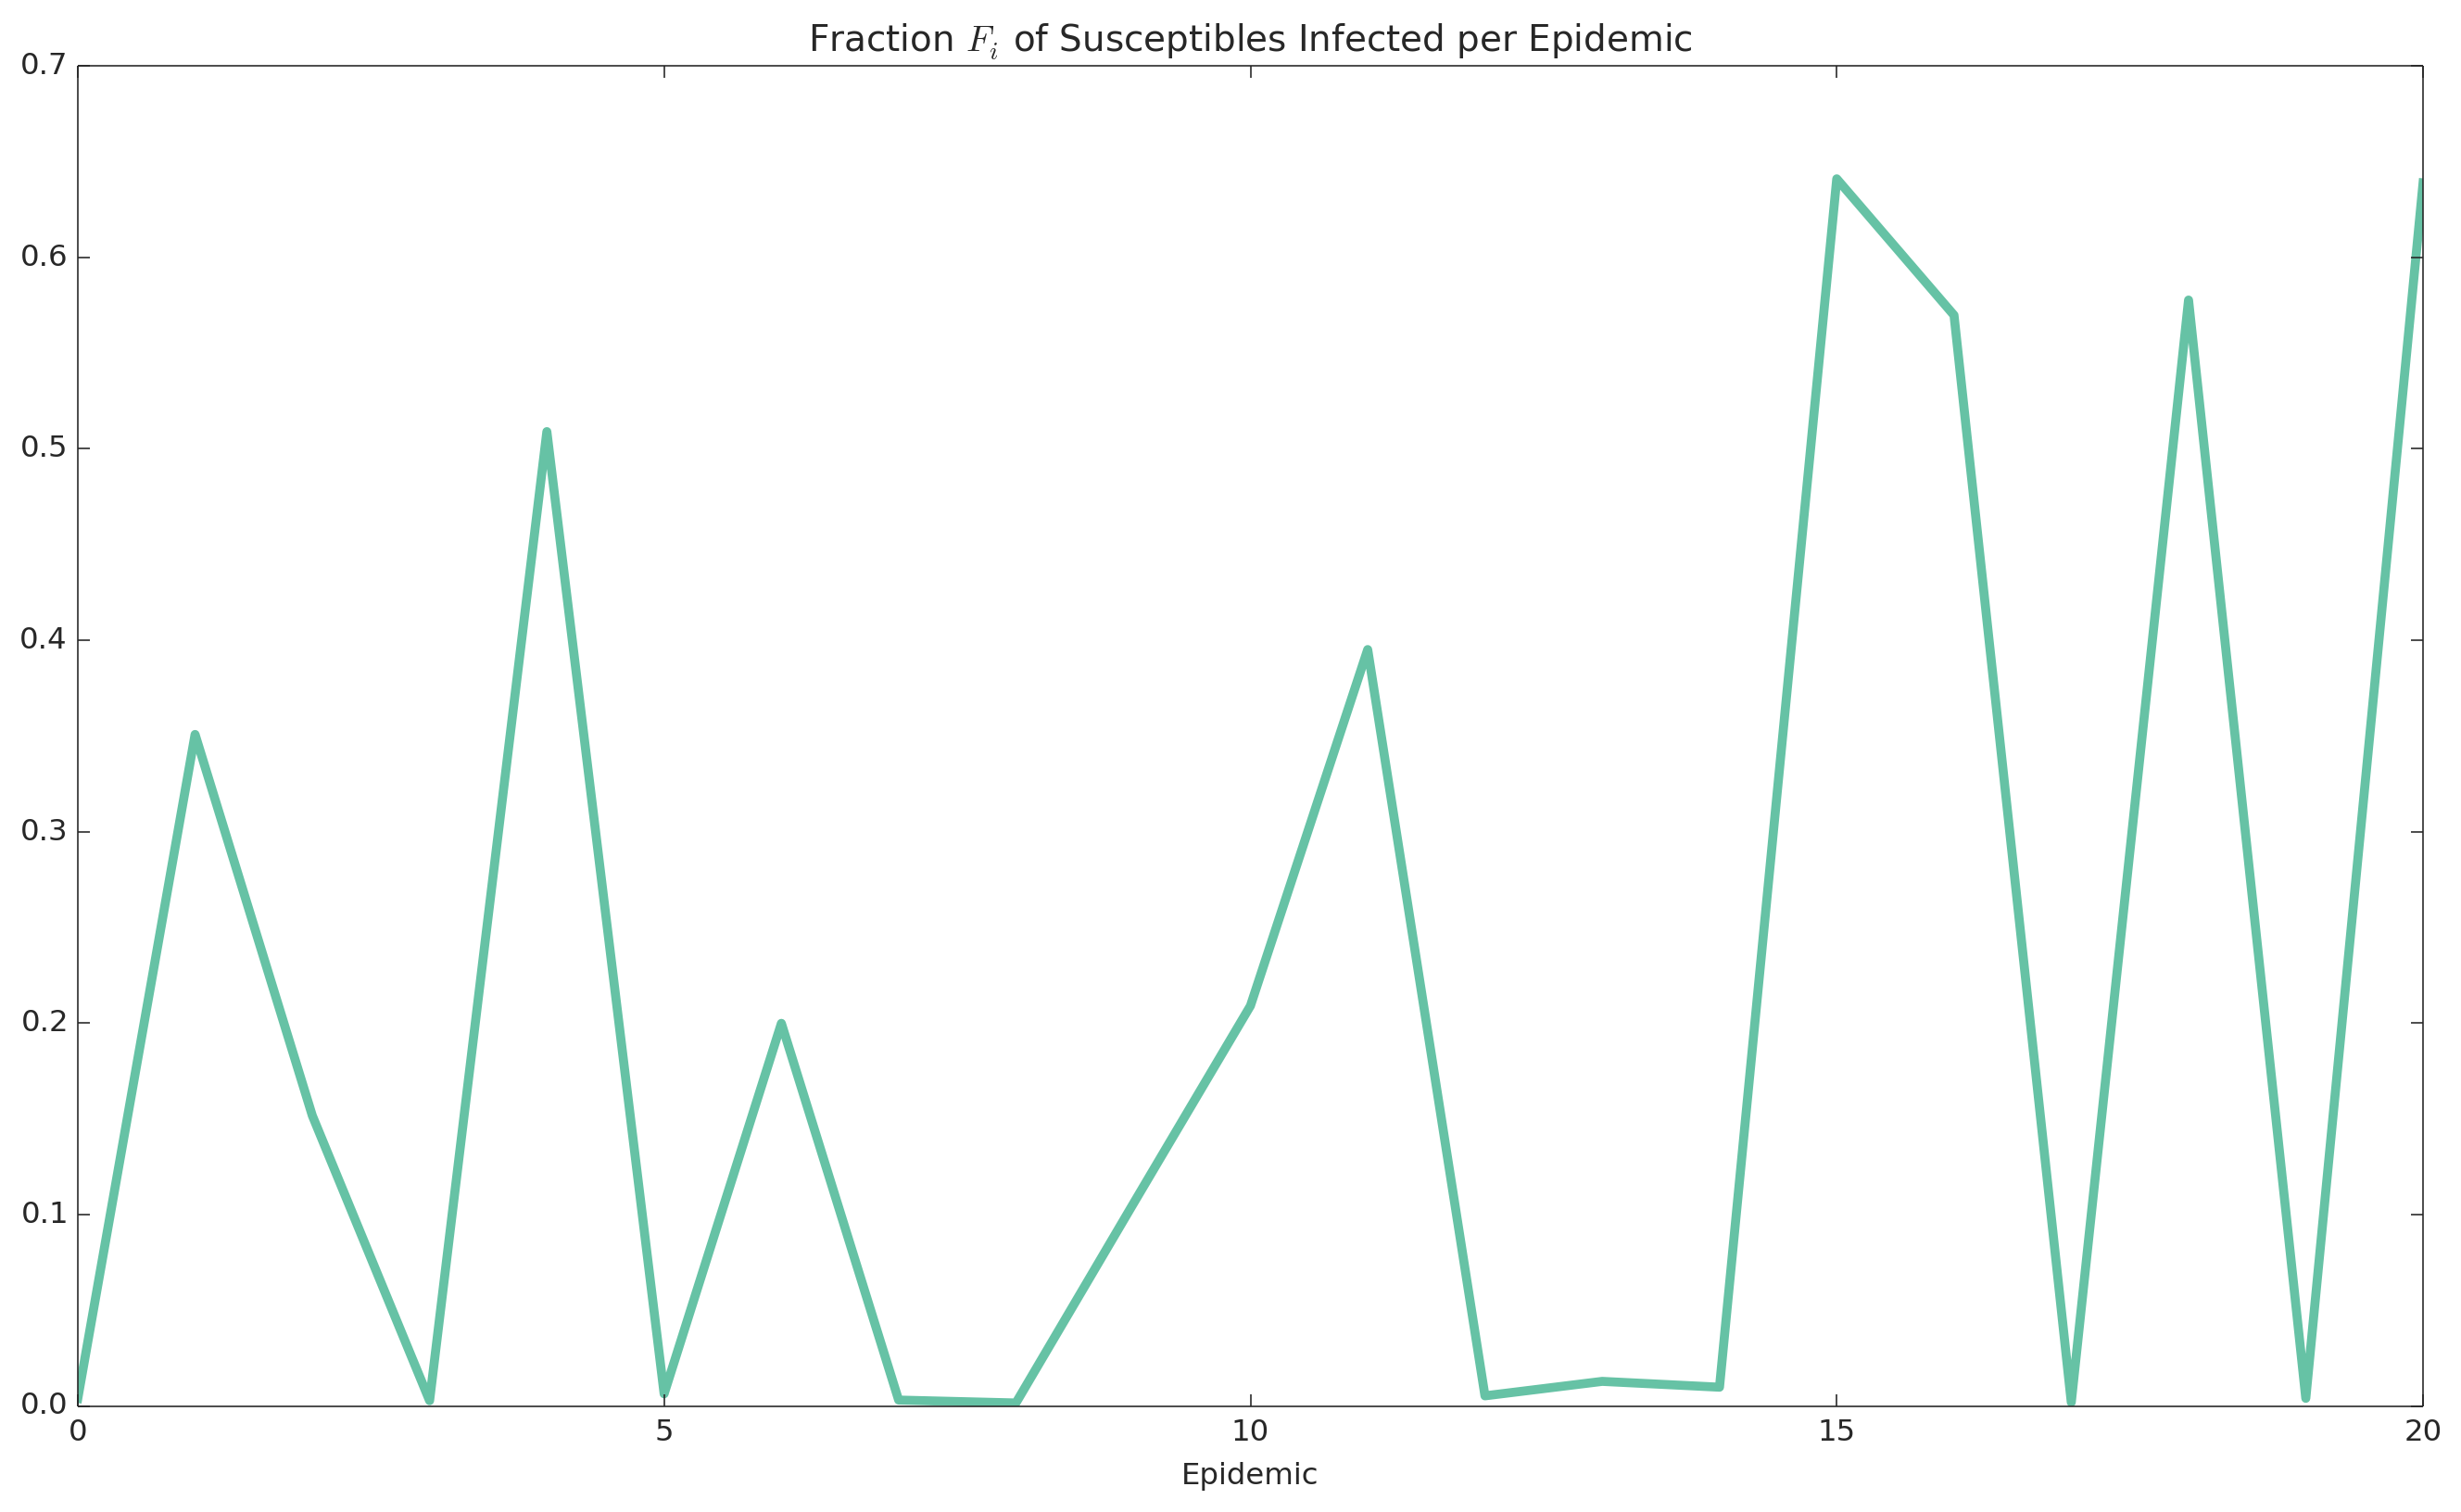
\includegraphics[max size={\textwidth}{\textheight}]{notebook_files/notebook_20_0.png}
    \par
    \end{center}
    
            \end{InvisibleVerbatim}
            
        
    


    % Make sure that atleast 4 lines are below the HR
    \needspace{4\baselineskip}

    
        \vspace{6pt}
        \makebox[0.1\linewidth]{\smaller\hfill\tt\color{nbframe-in-prompt}In\hspace{4pt}{[}233{]}:\hspace{4pt}}\\*
        \vspace{-2.65\baselineskip}
        \begin{ColorVerbatim}
            \vspace{-0.7\baselineskip}
            \begin{Verbatim}[commandchars=\\\{\}]

\end{Verbatim}

            
                \vspace{0.3\baselineskip}
            
        \end{ColorVerbatim}
    
\textbf{Scaling Relations}

As in Rhodes and Anderson (1996) \emph{Nature}, and Rhodes and Anderson
(1996) \emph{Proceedings of the Royal Society B}, we can analyse the
scaling relation of the sizes and the durations of epidemics as a
function of their frequencies. Rhodes and Anderson find power law (
scale-free ) for both size and duration; if that is the case, the bottom
two plots here should be linear, as these are on a log-log scale. The
top two plots are log-linear, and a straight line on these plots implies
an exponential ( scaled ) relationship.

    % Make sure that atleast 4 lines are below the HR
    \needspace{4\baselineskip}

    
        \vspace{6pt}
        \makebox[0.1\linewidth]{\smaller\hfill\tt\color{nbframe-in-prompt}In\hspace{4pt}{[}256{]}:\hspace{4pt}}\\*
        \vspace{-2.65\baselineskip}
        \begin{ColorVerbatim}
            \vspace{-0.7\baselineskip}
            \begin{Verbatim}[commandchars=\\\{\}]
\PY{c}{\PYZsh{} Calculate size and duration of each epidemic}
\PY{n}{sizes} \PY{o}{=} \PY{p}{[}\PY{n}{np}\PY{o}{.}\PY{n}{sum}\PY{p}{(}\PY{n}{C}\PY{p}{[}\PY{n}{e}\PY{p}{]} \PY{o}{*} \PY{n}{rho}\PY{p}{[}\PY{n}{e}\PY{p}{]}\PY{p}{)} \PY{k}{for} \PY{n}{e} \PY{o+ow}{in} \PY{n}{epi}\PY{p}{]}
\PY{n}{durations} \PY{o}{=} \PY{p}{[}\PY{n+nb}{len}\PY{p}{(}\PY{n}{e}\PY{p}{)} \PY{k}{for} \PY{n}{e} \PY{o+ow}{in} \PY{n}{epi}\PY{p}{]}



\PY{c}{\PYZsh{} Sizes of Epidemics}
\PY{n}{xs} \PY{o}{=} \PY{n}{np}\PY{o}{.}\PY{n}{sort}\PY{p}{(}\PY{n}{sizes}\PY{p}{)}\PY{o}{.}\PY{n}{reshape}\PY{p}{(}\PY{n+nb}{len}\PY{p}{(}\PY{n}{sizes}\PY{p}{)}\PY{p}{,} \PY{l+m+mi}{1}\PY{p}{)}
\PY{n}{ys} \PY{o}{=} \PY{n}{np}\PY{o}{.}\PY{n}{arange}\PY{p}{(}\PY{n+nb}{len}\PY{p}{(}\PY{n}{xs}\PY{p}{)}\PY{p}{)}\PY{p}{[}\PY{p}{:}\PY{p}{:}\PY{o}{\PYZhy{}}\PY{l+m+mi}{1}\PY{p}{]} \PY{o}{+} \PY{l+m+mi}{1}
\PY{n}{lxs} \PY{o}{=} \PY{n}{np}\PY{o}{.}\PY{n}{log}\PY{p}{(}\PY{n}{xs}\PY{p}{)}
\PY{n}{lys} \PY{o}{=} \PY{n}{np}\PY{o}{.}\PY{n}{log}\PY{p}{(}\PY{n}{ys}\PY{p}{)}

\PY{c}{\PYZsh{} Durations of Epidemics}
\PY{n}{xd} \PY{o}{=} \PY{n}{np}\PY{o}{.}\PY{n}{sort}\PY{p}{(}\PY{n}{durations}\PY{p}{)}\PY{o}{.}\PY{n}{reshape}\PY{p}{(}\PY{n+nb}{len}\PY{p}{(}\PY{n}{sizes}\PY{p}{)}\PY{p}{,} \PY{l+m+mi}{1}\PY{p}{)}
\PY{n}{yd} \PY{o}{=} \PY{n}{np}\PY{o}{.}\PY{n}{arange}\PY{p}{(}\PY{n+nb}{len}\PY{p}{(}\PY{n}{xd}\PY{p}{)}\PY{p}{)}\PY{p}{[}\PY{p}{:}\PY{p}{:}\PY{o}{\PYZhy{}}\PY{l+m+mi}{1}\PY{p}{]} \PY{o}{+} \PY{l+m+mi}{1}
\PY{n}{lxd} \PY{o}{=} \PY{n}{np}\PY{o}{.}\PY{n}{log}\PY{p}{(}\PY{n}{xd}\PY{p}{)}
\PY{n}{lyd} \PY{o}{=} \PY{n}{np}\PY{o}{.}\PY{n}{log}\PY{p}{(}\PY{n}{yd}\PY{p}{)}



\PY{n}{loglins} \PY{o}{=} \PY{n}{linear\PYZus{}model}\PY{o}{.}\PY{n}{BayesianRidge}\PY{p}{(}\PY{p}{)}
\PY{n}{loglogs} \PY{o}{=} \PY{n}{linear\PYZus{}model}\PY{o}{.}\PY{n}{BayesianRidge}\PY{p}{(}\PY{p}{)}
\PY{n}{loglind} \PY{o}{=} \PY{n}{linear\PYZus{}model}\PY{o}{.}\PY{n}{BayesianRidge}\PY{p}{(}\PY{p}{)}
\PY{n}{loglogd} \PY{o}{=} \PY{n}{linear\PYZus{}model}\PY{o}{.}\PY{n}{BayesianRidge}\PY{p}{(}\PY{p}{)}

\PY{n}{loglins}\PY{o}{.}\PY{n}{fit}\PY{p}{(}\PY{n}{xs}\PY{p}{,} \PY{n}{lys}\PY{p}{)}
\PY{n}{loglogs}\PY{o}{.}\PY{n}{fit}\PY{p}{(}\PY{n}{lxs}\PY{p}{,} \PY{n}{lys}\PY{p}{)}
\PY{n}{loglind}\PY{o}{.}\PY{n}{fit}\PY{p}{(}\PY{n}{xd}\PY{p}{,} \PY{n}{lyd}\PY{p}{)}
\PY{n}{loglogd}\PY{o}{.}\PY{n}{fit}\PY{p}{(}\PY{n}{lxd}\PY{p}{,} \PY{n}{lyd}\PY{p}{)}



\PY{n}{subplot}\PY{p}{(}\PY{l+m+mi}{221}\PY{p}{)}
\PY{n}{plt}\PY{o}{.}\PY{n}{semilogy}\PY{p}{(}\PY{n}{xs}\PY{p}{,} \PY{n}{ys}\PY{p}{,} \PY{l+s}{\PYZdq{}}\PY{l+s}{k.}\PY{l+s}{\PYZdq{}}\PY{p}{,} \PY{n}{ms}\PY{o}{=}\PY{l+m+mi}{12}\PY{p}{)}
\PY{n}{plt}\PY{o}{.}\PY{n}{semilogy}\PY{p}{(}\PY{n}{xs}\PY{p}{,} \PY{n}{np}\PY{o}{.}\PY{n}{exp}\PY{p}{(}\PY{n}{loglins}\PY{o}{.}\PY{n}{predict}\PY{p}{(}\PY{n}{xs}\PY{p}{)}\PY{p}{)}\PY{p}{,} \PY{n}{linewidth}\PY{o}{=}\PY{l+m+mi}{3}\PY{p}{)}
\PY{n}{title}\PY{p}{(}\PY{l+s}{\PYZdq{}}\PY{l+s}{Size}\PY{l+s}{\PYZdq{}}\PY{p}{)}
\PY{n}{ylabel}\PY{p}{(}\PY{l+s}{\PYZdq{}}\PY{l+s}{Log\PYZhy{}Linear}\PY{l+s}{\PYZdq{}}\PY{p}{)}

\PY{n}{subplot}\PY{p}{(}\PY{l+m+mi}{222}\PY{p}{)}
\PY{n}{plt}\PY{o}{.}\PY{n}{semilogy}\PY{p}{(}\PY{n}{xd}\PY{p}{,} \PY{n}{yd}\PY{p}{,} \PY{l+s}{\PYZdq{}}\PY{l+s}{k.}\PY{l+s}{\PYZdq{}}\PY{p}{,} \PY{n}{ms}\PY{o}{=}\PY{l+m+mi}{12}\PY{p}{)}
\PY{n}{plt}\PY{o}{.}\PY{n}{semilogy}\PY{p}{(}\PY{n}{xd}\PY{p}{,} \PY{n}{np}\PY{o}{.}\PY{n}{exp}\PY{p}{(}\PY{n}{loglind}\PY{o}{.}\PY{n}{predict}\PY{p}{(}\PY{n}{xd}\PY{p}{)}\PY{p}{)}\PY{p}{,} \PY{n}{linewidth}\PY{o}{=}\PY{l+m+mi}{3}\PY{p}{)}
\PY{n}{title}\PY{p}{(}\PY{l+s}{\PYZdq{}}\PY{l+s}{Duration}\PY{l+s}{\PYZdq{}}\PY{p}{)}

\PY{n}{subplot}\PY{p}{(}\PY{l+m+mi}{223}\PY{p}{)}
\PY{n}{plt}\PY{o}{.}\PY{n}{loglog}\PY{p}{(}\PY{n}{xs}\PY{p}{,} \PY{n}{ys}\PY{p}{,} \PY{l+s}{\PYZdq{}}\PY{l+s}{k.}\PY{l+s}{\PYZdq{}}\PY{p}{,} \PY{n}{ms}\PY{o}{=}\PY{l+m+mi}{12}\PY{p}{)}
\PY{n}{plt}\PY{o}{.}\PY{n}{loglog}\PY{p}{(}\PY{n}{np}\PY{o}{.}\PY{n}{exp}\PY{p}{(}\PY{n}{lxs}\PY{p}{)}\PY{p}{,} \PY{n}{np}\PY{o}{.}\PY{n}{exp}\PY{p}{(}\PY{n}{loglogs}\PY{o}{.}\PY{n}{predict}\PY{p}{(}\PY{n}{lxs}\PY{p}{)}\PY{p}{)}\PY{p}{,} \PY{n}{linewidth}\PY{o}{=}\PY{l+m+mi}{3}\PY{p}{)}
\PY{n}{ylabel}\PY{p}{(}\PY{l+s}{\PYZdq{}}\PY{l+s}{Log\PYZhy{}Log}\PY{l+s}{\PYZdq{}}\PY{p}{)}

\PY{n}{subplot}\PY{p}{(}\PY{l+m+mi}{224}\PY{p}{)}
\PY{n}{plt}\PY{o}{.}\PY{n}{loglog}\PY{p}{(}\PY{n}{xd}\PY{p}{,} \PY{n}{yd}\PY{p}{,} \PY{l+s}{\PYZdq{}}\PY{l+s}{k.}\PY{l+s}{\PYZdq{}}\PY{p}{,} \PY{n}{ms}\PY{o}{=}\PY{l+m+mi}{12}\PY{p}{)}
\PY{n}{plt}\PY{o}{.}\PY{n}{loglog}\PY{p}{(}\PY{n}{np}\PY{o}{.}\PY{n}{exp}\PY{p}{(}\PY{n}{lxd}\PY{p}{)}\PY{p}{,} \PY{n}{np}\PY{o}{.}\PY{n}{exp}\PY{p}{(}\PY{n}{loglogd}\PY{o}{.}\PY{n}{predict}\PY{p}{(}\PY{n}{lxd}\PY{p}{)}\PY{p}{)}\PY{p}{,} \PY{n}{linewidth}\PY{o}{=}\PY{l+m+mi}{3}\PY{p}{)}

\PY{c}{\PYZsh{}plt.scatter(sizes, durations)}
\end{Verbatim}

            
                \vspace{-0.2\baselineskip}
            
        \end{ColorVerbatim}
    

    

        % If the first block is an image, minipage the image.  Else
        % request a certain amount of space for the input text.
        \needspace{4\baselineskip}
        
        

            % Add document contents.
            
                \makebox[0.1\linewidth]{\smaller\hfill\tt\color{nbframe-out-prompt}Out\hspace{4pt}{[}256{]}:\hspace{4pt}}\\*
                \vspace{-2.55\baselineskip}\begin{InvisibleVerbatim}
                \vspace{-0.5\baselineskip}
\begin{alltt}[<matplotlib.lines.Line2D at 0x138d7f990>]\end{alltt}

            \end{InvisibleVerbatim}
            
                \begin{InvisibleVerbatim}
                \vspace{-0.5\baselineskip}
    \begin{center}
    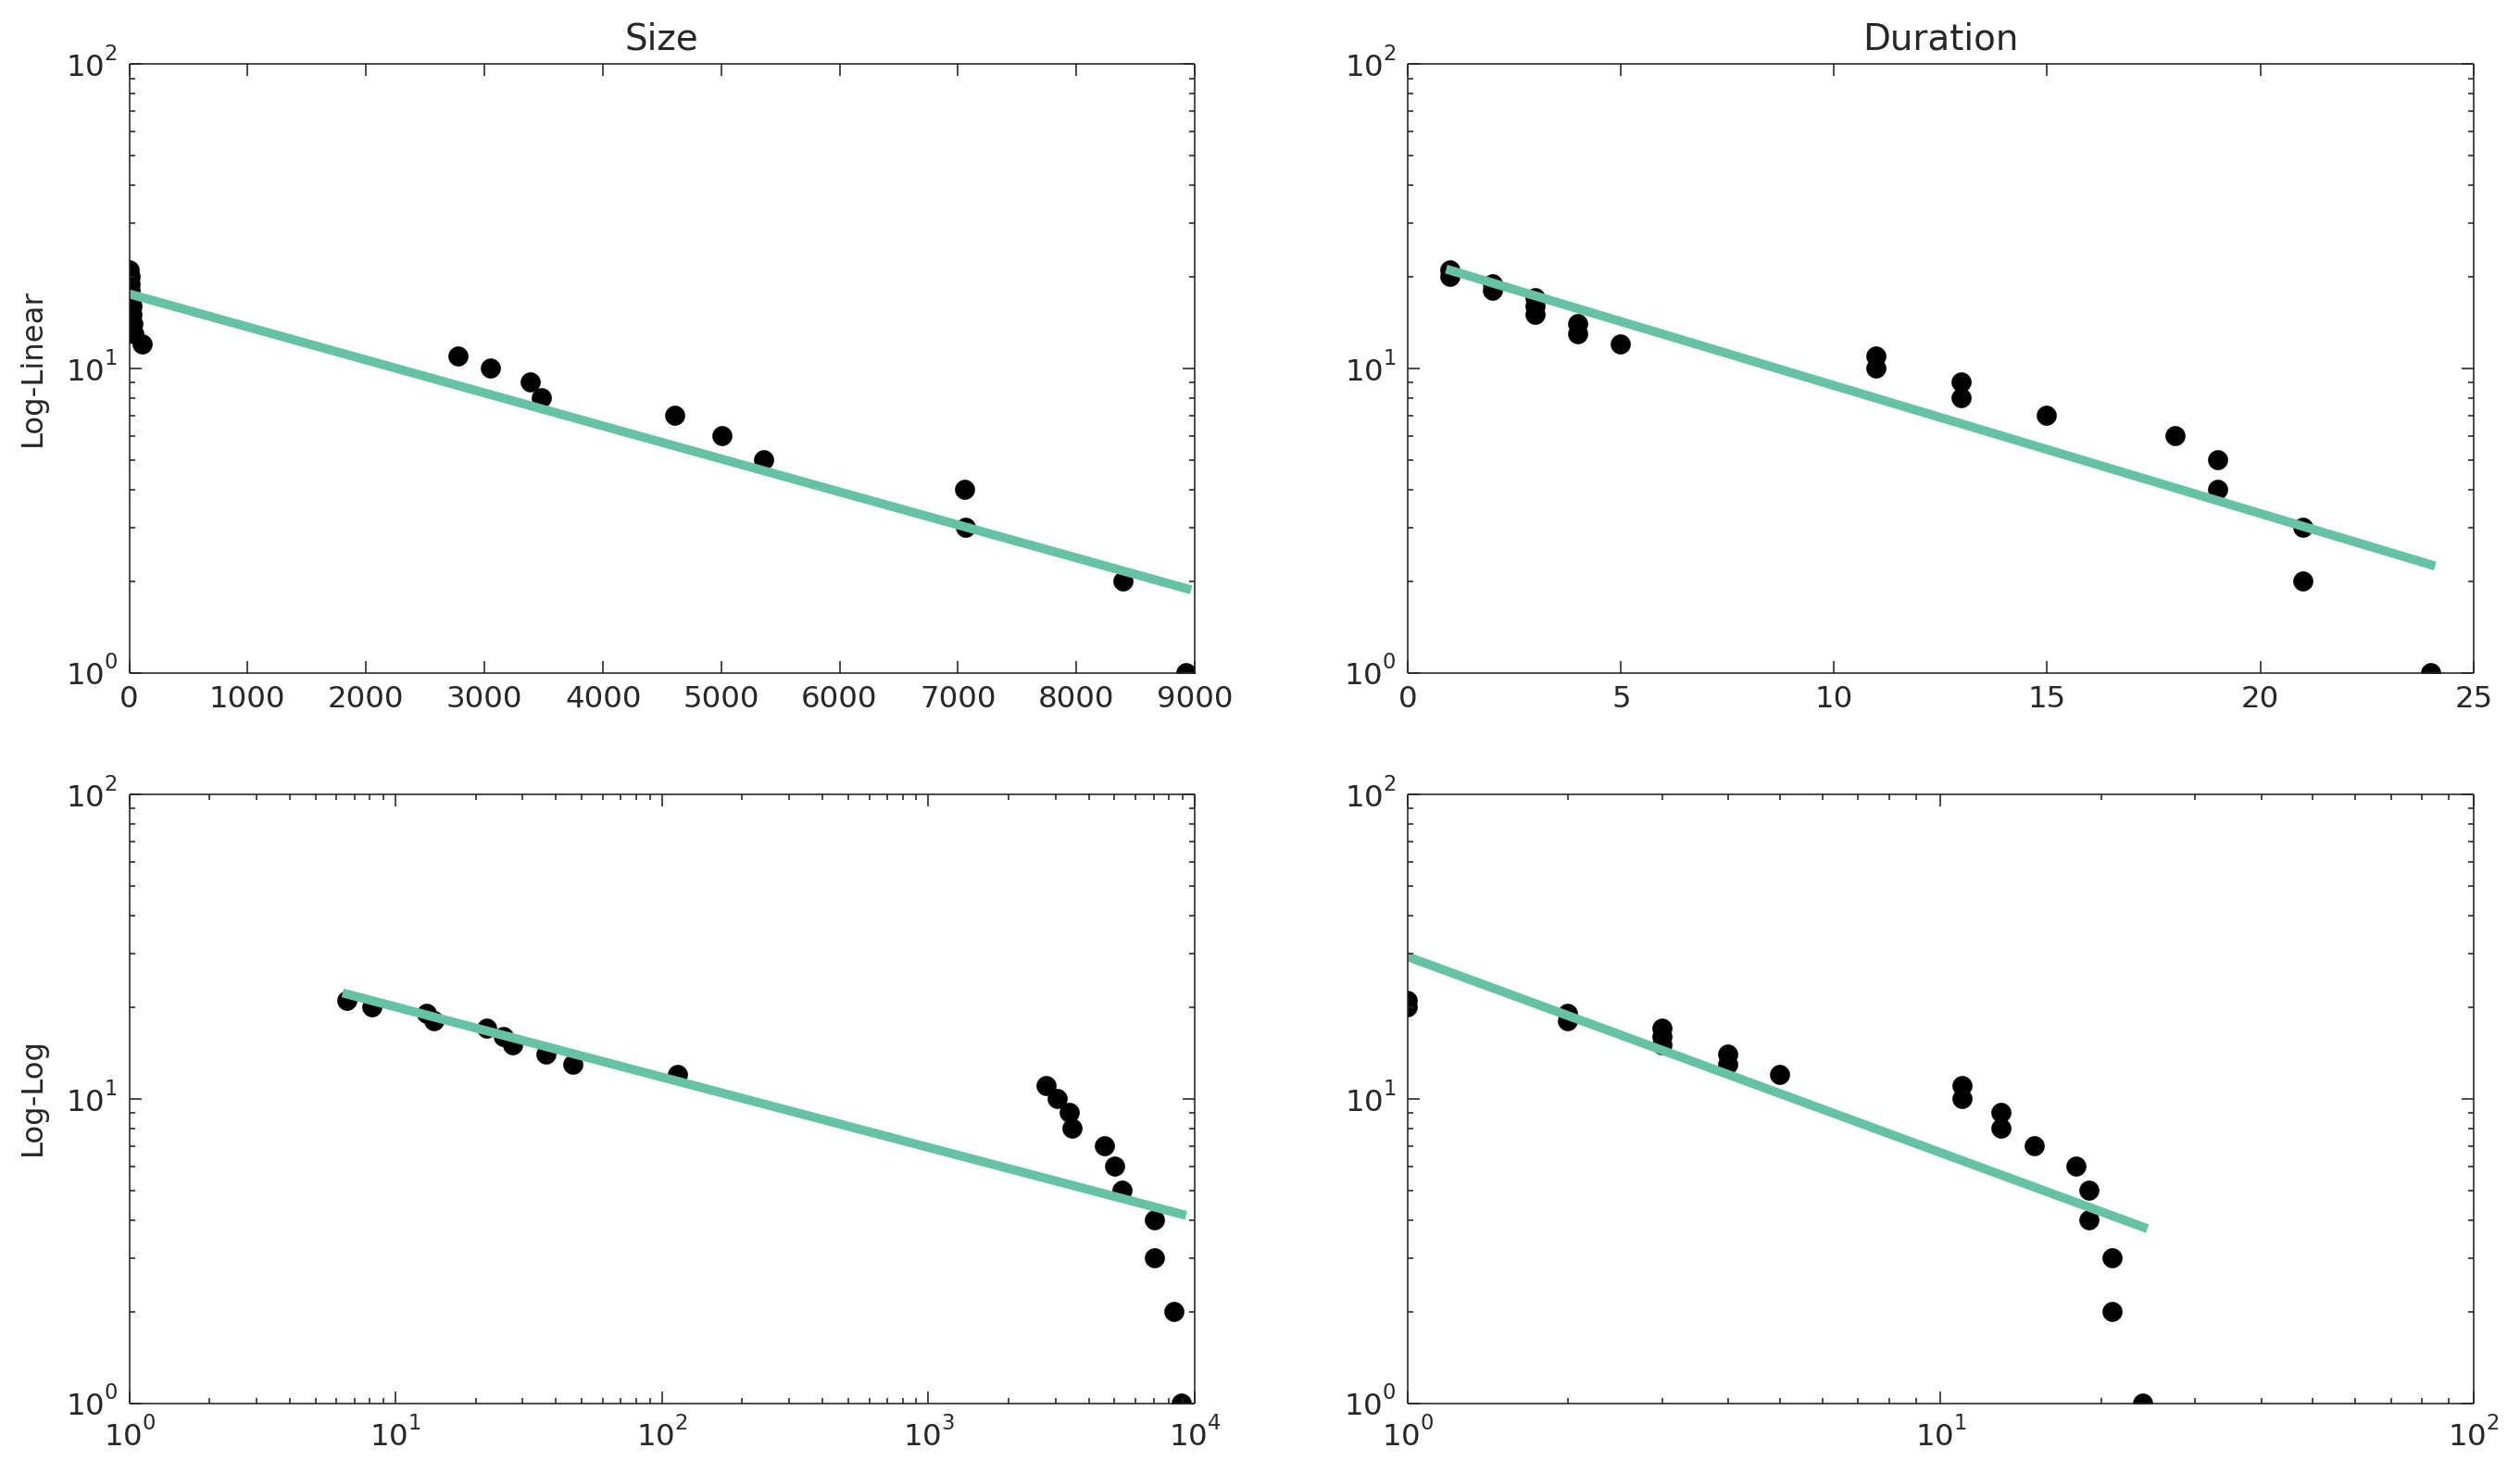
\includegraphics[max size={\textwidth}{\textheight}]{notebook_files/notebook_23_1.png}
    \par
    \end{center}
    
            \end{InvisibleVerbatim}
            
        
    
\textbf{TSIR Fitting on Simulated Data}

We have all relevant parameters to simulate a new set of epidemics using
the TSIR model, assuming small populations. If the above system is for a
large population, this cell will do nothing.

In order to spark the epidemics, we need to infer the rate of
importation of cases into the population. We will separate this into two
processes : a low-mean Poisson rate of importation, which will determine
the \emph{timing} of the imports, and a beta distribution of import
\emph{sizes}.

As before, we're assuming that the epidemic goes extinct once it drops
below sensitivity. If this is not assumed, we get very small
oscillations and the disease looks to be endemic - the same happens if
we fit a the TSIR to the observed data above and predict.

This cell runs most of the code above. After generating simulated data,
it fits it and calculates predictions in the same manner. All plots are
skipped, except the one of predicted vs actual epidemic size.

    % Make sure that atleast 4 lines are below the HR
    \needspace{4\baselineskip}

    
        \vspace{6pt}
        \makebox[0.1\linewidth]{\smaller\hfill\tt\color{nbframe-in-prompt}In\hspace{4pt}{[}234{]}:\hspace{4pt}}\\*
        \vspace{-2.65\baselineskip}
        \begin{ColorVerbatim}
            \vspace{-0.7\baselineskip}
            \begin{Verbatim}[commandchars=\\\{\}]

\end{Verbatim}

            
                \vspace{0.3\baselineskip}
            
        \end{ColorVerbatim}
    


    % Make sure that atleast 4 lines are below the HR
    \needspace{4\baselineskip}

    
        \vspace{6pt}
        \makebox[0.1\linewidth]{\smaller\hfill\tt\color{nbframe-in-prompt}In\hspace{4pt}{[}235{]}:\hspace{4pt}}\\*
        \vspace{-2.65\baselineskip}
        \begin{ColorVerbatim}
            \vspace{-0.7\baselineskip}
            \begin{Verbatim}[commandchars=\\\{\}]
\PY{c}{\PYZsh{} If we\PYZsq{}re in a small population }
\PY{k}{if} \PY{p}{(}\PY{n}{np}\PY{o}{.}\PY{n}{sum}\PY{p}{(}\PY{n}{C} \PY{o}{\PYZlt{}}\PY{o}{=} \PY{n}{sensitivity}\PY{p}{)}\PY{o}{.}\PY{n}{astype}\PY{p}{(}\PY{n+nb}{float}\PY{p}{)} \PY{o}{/} \PY{n+nb}{len}\PY{p}{(}\PY{n}{C}\PY{p}{)}\PY{p}{)} \PY{o}{\PYZgt{}} \PY{l+m+mf}{0.5} \PY{p}{:}
        
    \PY{c}{\PYZsh{} Let\PYZsq{}s generate a Poisson realisation with the same parameterisation}
    \PY{c}{\PYZsh{} We\PYZsq{}ll make it longer than the previous series, to allow it to equilibriate}
    \PY{n}{simpoi} \PY{o}{=} \PY{n}{np}\PY{o}{.}\PY{n}{array}\PY{p}{(}\PY{n}{st}\PY{o}{.}\PY{n}{poisson}\PY{p}{(}\PY{n+nb}{float}\PY{p}{(}\PY{n+nb}{len}\PY{p}{(}\PY{n}{epi}\PY{p}{)}\PY{p}{)} \PY{o}{/} \PY{n+nb}{len}\PY{p}{(}\PY{n}{C}\PY{p}{)}\PY{p}{)}\PY{o}{.}\PY{n}{rvs}\PY{p}{(}\PY{n+nb}{len}\PY{p}{(}\PY{n}{C}\PY{p}{)} \PY{o}{*} \PY{l+m+mi}{20}\PY{p}{)}\PY{p}{)}\PY{o}{.}\PY{n}{astype}\PY{p}{(}\PY{n+nb}{float}\PY{p}{)}
    
    
    
    \PY{c}{\PYZsh{} Next, let\PYZsq{}s find the distribution of import sizes, assumed to be exponential}
    \PY{c}{\PYZsh{} First, let\PYZsq{}s collect the size of each spark}
    \PY{n}{obsbeta} \PY{o}{=} \PY{p}{[}\PY{n}{C}\PY{p}{[}\PY{n}{i}\PY{p}{[}\PY{l+m+mi}{0}\PY{p}{]}\PY{p}{]} \PY{k}{for} \PY{n}{i} \PY{o+ow}{in} \PY{n}{epi}\PY{p}{]}
    
    \PY{c}{\PYZsh{} Next, fit to an exponential using maximum likelihood}
    \PY{c}{\PYZsh{} WARNING : the statistical power here is going to be dubious at best, with such a small amount of data...}
    \PY{n}{betafit} \PY{o}{=} \PY{n}{st}\PY{o}{.}\PY{n}{beta}\PY{o}{.}\PY{n}{fit}\PY{p}{(}\PY{n}{obsbeta}\PY{p}{)}
    
    \PY{c}{\PYZsh{} We can now generate some random variables to give sizes to our imports}
    \PY{n}{simbeta} \PY{o}{=} \PY{n}{st}\PY{o}{.}\PY{n}{beta}\PY{p}{(}\PY{n}{betafit}\PY{p}{[}\PY{l+m+mi}{0}\PY{p}{]}\PY{p}{,} \PY{n}{betafit}\PY{p}{[}\PY{l+m+mi}{1}\PY{p}{]}\PY{p}{,} \PY{n}{loc}\PY{o}{=}\PY{n}{betafit}\PY{p}{[}\PY{l+m+mi}{2}\PY{p}{]}\PY{p}{,} \PY{n}{scale}\PY{o}{=}\PY{n}{betafit}\PY{p}{[}\PY{l+m+mi}{3}\PY{p}{]}\PY{p}{)}\PY{o}{.}\PY{n}{rvs}\PY{p}{(}\PY{n}{np}\PY{o}{.}\PY{n}{sum}\PY{p}{(}\PY{n}{simpoi}\PY{p}{)}\PY{p}{)}
    
    
    
    \PY{c}{\PYZsh{} Putting them together :}
    \PY{n}{starts2} \PY{o}{=} \PY{n}{np}\PY{o}{.}\PY{n}{where}\PY{p}{(}\PY{n}{simpoi} \PY{o}{==} \PY{l+m+mi}{1}\PY{p}{)}\PY{p}{[}\PY{l+m+mi}{0}\PY{p}{]}
    \PY{k}{for} \PY{n}{i}\PY{p}{,} \PY{n}{j} \PY{o+ow}{in} \PY{n+nb}{enumerate}\PY{p}{(}\PY{n}{starts2}\PY{p}{)} \PY{p}{:}
        \PY{n}{simpoi}\PY{p}{[}\PY{n}{j}\PY{p}{]} \PY{o}{=} \PY{n}{simbeta}\PY{p}{[}\PY{n}{i}\PY{p}{]} \PY{c}{\PYZsh{}/ 10.\PYZsh{}np.mean(rho)}
    
    \PY{n}{subplot}\PY{p}{(}\PY{l+m+mi}{311}\PY{p}{)}
    \PY{n}{plt}\PY{o}{.}\PY{n}{plot}\PY{p}{(}\PY{n}{simpoi}\PY{p}{[}\PY{o}{\PYZhy{}}\PY{l+m+mi}{10}\PY{o}{*}\PY{n+nb}{len}\PY{p}{(}\PY{n}{C}\PY{p}{)}\PY{p}{:}\PY{p}{]}\PY{p}{,} \PY{n}{linewidth}\PY{o}{=}\PY{l+m+mi}{3}\PY{p}{)}
    \PY{n}{title}\PY{p}{(}\PY{l+s}{\PYZdq{}}\PY{l+s}{Seeded Epidemic Sparks}\PY{l+s}{\PYZdq{}}\PY{p}{)}
        
    
    \PY{c}{\PYZsh{} Let\PYZsq{}s predict a TSIR based on this series of imports}
    \PY{c}{\PYZsh{} Initialise S, with the first value at Sbar}
    \PY{n}{simS} \PY{o}{=} \PY{n}{np}\PY{o}{.}\PY{n}{zeros\PYZus{}like}\PY{p}{(}\PY{n}{simpoi}\PY{p}{)}
    \PY{n}{simS}\PY{p}{[}\PY{l+m+mi}{0}\PY{p}{]} \PY{o}{=} \PY{n+nb}{float}\PY{p}{(}\PY{n}{Sbar}\PY{p}{)}
    
    \PY{c}{\PYZsh{} We need to extrapolate births. Just for the first test, we\PYZsq{}ll just keep any future values at the last known value}
    \PY{n}{BB} \PY{o}{=} \PY{n}{np}\PY{o}{.}\PY{n}{append}\PY{p}{(}\PY{n}{B}\PY{p}{,} \PY{n}{np}\PY{o}{.}\PY{n}{ones}\PY{p}{(}\PY{n+nb}{len}\PY{p}{(}\PY{n}{B}\PY{p}{)}\PY{o}{*}\PY{l+m+mi}{19}\PY{p}{)} \PY{o}{*} \PY{n}{B}\PY{p}{[}\PY{o}{\PYZhy{}}\PY{l+m+mi}{1}\PY{p}{]}\PY{p}{)}

    \PY{c}{\PYZsh{} Simulating ...}
    \PY{k}{for} \PY{n}{i} \PY{o+ow}{in} \PY{n+nb}{range}\PY{p}{(}\PY{l+m+mi}{1}\PY{p}{,} \PY{n+nb}{len}\PY{p}{(}\PY{n}{C}\PY{p}{)}\PY{o}{*}\PY{l+m+mi}{20}\PY{p}{)} \PY{p}{:}
        
        \PY{c}{\PYZsh{} If we\PYZsq{}re not forcing imports}
        \PY{k}{if} \PY{n}{i} \PY{o+ow}{not} \PY{o+ow}{in} \PY{n}{starts2} \PY{p}{:}
            \PY{n}{simpoi}\PY{p}{[}\PY{n}{i}\PY{p}{]} \PY{o}{=} \PY{n}{r}\PY{p}{[}\PY{n}{i} \PY{o}{\PYZpc{}} \PY{n}{periodicity}\PY{p}{]} \PY{o}{*} \PY{p}{(} \PY{n}{simpoi}\PY{p}{[}\PY{n}{i}\PY{o}{\PYZhy{}}\PY{l+m+mi}{1}\PY{p}{]} \PY{o}{*}\PY{o}{*} \PY{n}{alphaSbar} \PY{p}{)} \PY{o}{*} \PY{n}{simS}\PY{p}{[}\PY{n}{i}\PY{o}{\PYZhy{}}\PY{l+m+mi}{1}\PY{p}{]}
        
            \PY{k}{if} \PY{n}{simpoi}\PY{p}{[}\PY{n}{i}\PY{p}{]} \PY{o}{\PYZlt{}} \PY{n}{sensitivity} \PY{p}{:}
                \PY{n}{simpoi}\PY{p}{[}\PY{n}{i}\PY{p}{]} \PY{o}{=} \PY{l+m+mi}{0}
        
        \PY{n}{simS}\PY{p}{[}\PY{n}{i}\PY{p}{]} \PY{o}{=} \PY{n}{BB}\PY{p}{[}\PY{n+nb}{max}\PY{p}{(}\PY{n}{i} \PY{o}{\PYZhy{}} \PY{n}{delay}\PY{p}{,} \PY{l+m+mi}{0}\PY{p}{)}\PY{p}{]} \PY{o}{+} \PY{n}{simS}\PY{p}{[}\PY{n}{i}\PY{o}{\PYZhy{}}\PY{l+m+mi}{1}\PY{p}{]} \PY{o}{\PYZhy{}} \PY{n}{simpoi}\PY{p}{[}\PY{n}{i}\PY{p}{]}
        
    \PY{l+s+sd}{\PYZdq{}\PYZdq{}\PYZdq{}    }
\PY{l+s+sd}{    \PYZsh{} Plots}
\PY{l+s+sd}{    subplot(312)}
\PY{l+s+sd}{    plt.plot(simpoi[\PYZhy{}len(C):], linewidth=3)}
\PY{l+s+sd}{    title(\PYZdq{}Simulated Epidemics After Equilibration\PYZdq{})}
\PY{l+s+sd}{    }
\PY{l+s+sd}{    subplot(313)}
\PY{l+s+sd}{    plt.plot(simS[\PYZhy{}len(C):], linewidth=3)}
\PY{l+s+sd}{    axhline(Sbar, color=\PYZdq{}red\PYZdq{}, linewidth=2)}
\PY{l+s+sd}{    title(\PYZdq{}Susceptibles\PYZdq{})}
\PY{l+s+sd}{    legend([\PYZdq{}Susceptibles\PYZdq{}, \PYZdq{}Original Sbar\PYZdq{}])}
\PY{l+s+sd}{    }
\PY{l+s+sd}{    tight\PYZus{}layout()}
\PY{l+s+sd}{    \PYZdq{}\PYZdq{}\PYZdq{}}

    
    
    \PY{c}{\PYZsh{} With the data generated, let\PYZsq{}s fit a TSIR to it ( discarding the first half as burn\PYZhy{}in )}
    \PY{c}{\PYZsh{} We should fine perfect reporting, so rho = 1}
     
    \PY{n}{D} \PY{o}{=} \PY{n}{simpoi}\PY{p}{[}\PY{n+nb}{len}\PY{p}{(}\PY{n}{simpoi}\PY{p}{)}\PY{o}{/}\PY{l+m+mi}{2}\PY{p}{:}\PY{p}{]}
        
    \PY{c}{\PYZsh{} Where are the epidemics ?}
    \PY{n}{epis} \PY{o}{=} \PY{p}{[}\PY{p}{]}
    
    \PY{c}{\PYZsh{} If there are many zeros ( here, we say at least 50\PYZpc{} ), we can cut epidemics naturally at non\PYZhy{}zeros}
    \PY{k}{if} \PY{p}{(}\PY{n}{np}\PY{o}{.}\PY{n}{sum}\PY{p}{(}\PY{n}{D} \PY{o}{\PYZlt{}}\PY{o}{=} \PY{n}{sensitivity}\PY{p}{)}\PY{o}{.}\PY{n}{astype}\PY{p}{(}\PY{n+nb}{float}\PY{p}{)} \PY{o}{/} \PY{n+nb}{len}\PY{p}{(}\PY{n}{D}\PY{p}{)}\PY{p}{)} \PY{o}{\PYZgt{}} \PY{l+m+mf}{0.5} \PY{p}{:}
        \PY{n}{zs} \PY{o}{=} \PY{n}{np}\PY{o}{.}\PY{n}{where}\PY{p}{(}\PY{n}{D} \PY{o}{\PYZgt{}} \PY{n}{sensitivity}\PY{p}{)}\PY{p}{[}\PY{l+m+mi}{0}\PY{p}{]} \PY{c}{\PYZsh{} Find epidemics over sensitivity threshold}
        \PY{n}{dzs} \PY{o}{=} \PY{n}{np}\PY{o}{.}\PY{n}{where}\PY{p}{(}\PY{n}{np}\PY{o}{.}\PY{n}{append}\PY{p}{(}\PY{n}{np}\PY{o}{.}\PY{n}{insert}\PY{p}{(}\PY{n}{np}\PY{o}{.}\PY{n}{diff}\PY{p}{(}\PY{n}{zs}\PY{p}{)}\PY{p}{,} \PY{l+m+mi}{0}\PY{p}{,} \PY{l+m+mi}{0}\PY{p}{)}\PY{p}{,} \PY{o}{\PYZhy{}}\PY{l+m+mi}{1}\PY{p}{)} \PY{o}{!=} \PY{l+m+mi}{1}\PY{p}{)}\PY{p}{[}\PY{l+m+mi}{0}\PY{p}{]}
        \PY{k}{for} \PY{n}{i} \PY{o+ow}{in} \PY{n+nb}{range}\PY{p}{(}\PY{n+nb}{len}\PY{p}{(}\PY{n}{dzs}\PY{p}{)}\PY{o}{\PYZhy{}}\PY{l+m+mi}{1}\PY{p}{)} \PY{p}{:}
            \PY{n}{epis}\PY{o}{.}\PY{n}{append}\PY{p}{(}\PY{n}{zs}\PY{p}{[}\PY{n}{dzs}\PY{p}{[}\PY{n}{i}\PY{p}{]}\PY{p}{:}\PY{n}{dzs}\PY{p}{[}\PY{n}{i}\PY{o}{+}\PY{l+m+mi}{1}\PY{p}{]}\PY{p}{]}\PY{p}{)}
          
    \PY{k}{else} \PY{p}{:} \PY{c}{\PYZsh{} Otherwise, slice at local minima using smoothed zero\PYZhy{}crossings in the derivative}
        \PY{n}{zs} \PY{o}{=} \PY{n+nb}{range}\PY{p}{(}\PY{n+nb}{len}\PY{p}{(}\PY{n}{simpoi}\PY{p}{)}\PY{p}{)}
        \PY{n}{z2s} \PY{o}{=} \PY{n}{np}\PY{o}{.}\PY{n}{diff}\PY{p}{(}\PY{n}{np}\PY{o}{.}\PY{n}{convolve}\PY{p}{(}\PY{n}{D}\PY{p}{,} \PY{n}{np}\PY{o}{.}\PY{n}{hanning}\PY{p}{(}\PY{l+m+mi}{19}\PY{p}{)}\PY{p}{,} \PY{l+s}{\PYZdq{}}\PY{l+s}{same}\PY{l+s}{\PYZdq{}}\PY{p}{)}\PY{p}{)}
        \PY{n}{dzs} \PY{o}{=} \PY{n}{np}\PY{o}{.}\PY{n}{append}\PY{p}{(}\PY{n}{np}\PY{o}{.}\PY{n}{insert}\PY{p}{(}\PY{p}{(}\PY{n}{np}\PY{o}{.}\PY{n}{where}\PY{p}{(}\PY{p}{(}\PY{n}{z2s}\PY{p}{[}\PY{p}{:}\PY{o}{\PYZhy{}}\PY{l+m+mi}{1}\PY{p}{]} \PY{o}{\PYZlt{}} \PY{l+m+mi}{0}\PY{p}{)} \PY{o}{*} \PY{p}{(}\PY{n}{z2s}\PY{p}{[}\PY{l+m+mi}{1}\PY{p}{:}\PY{p}{]} \PY{o}{\PYZgt{}} \PY{l+m+mi}{0}\PY{p}{)} \PY{o}{==} \PY{n+nb+bp}{True}\PY{p}{)}\PY{p}{[}\PY{l+m+mi}{0}\PY{p}{]}\PY{p}{)}\PY{p}{,} \PY{l+m+mi}{0}\PY{p}{,} \PY{l+m+mi}{0}\PY{p}{)}\PY{p}{,} \PY{n+nb}{len}\PY{p}{(}\PY{n}{D}\PY{p}{)}\PY{p}{)}
        \PY{k}{for} \PY{n}{i} \PY{o+ow}{in} \PY{n+nb}{range}\PY{p}{(}\PY{n+nb}{len}\PY{p}{(}\PY{n}{dzs}\PY{p}{)}\PY{o}{\PYZhy{}}\PY{l+m+mi}{1}\PY{p}{)} \PY{p}{:}
            \PY{n}{epis}\PY{o}{.}\PY{n}{append}\PY{p}{(}\PY{n+nb}{range}\PY{p}{(}\PY{n}{dzs}\PY{p}{[}\PY{n}{i}\PY{p}{]}\PY{p}{,} \PY{n}{dzs}\PY{p}{[}\PY{n}{i}\PY{o}{+}\PY{l+m+mi}{1}\PY{p}{]}\PY{p}{)}\PY{p}{)}
    
    \PY{n}{epis} \PY{o}{=} \PY{n}{np}\PY{o}{.}\PY{n}{array}\PY{p}{(}\PY{n}{epis}\PY{p}{)}
    
    
    
    \PY{n}{Ys} \PY{o}{=} \PY{n}{np}\PY{o}{.}\PY{n}{cumsum}\PY{p}{(}\PY{n}{BB}\PY{p}{[}\PY{o}{\PYZhy{}}\PY{n+nb}{len}\PY{p}{(}\PY{n}{D}\PY{p}{)}\PY{p}{:}\PY{p}{]}\PY{p}{)}
    \PY{n}{Xs} \PY{o}{=} \PY{n}{np}\PY{o}{.}\PY{n}{cumsum}\PY{p}{(}\PY{n}{D}\PY{p}{)} 
    
    
    \PY{c}{\PYZsh{} Compute rho ( rate of reporting ) using Bayesian ridge regression with a polynomial}
    \PY{n}{regs} \PY{o}{=} \PY{n}{linear\PYZus{}model}\PY{o}{.}\PY{n}{BayesianRidge}\PY{p}{(}\PY{n}{fit\PYZus{}intercept}\PY{o}{=}\PY{n+nb+bp}{False}\PY{p}{,} \PY{n}{compute\PYZus{}score}\PY{o}{=}\PY{n+nb+bp}{True}\PY{p}{)}
    
    \PY{c}{\PYZsh{} Compute the R\PYZca{}2 for a range of polynomials from degree\PYZhy{}1 to degree\PYZhy{}10}
    \PY{c}{\PYZsh{} The fit score has a penalty proportional to the square of the degree of the polynomial}
    \PY{n}{Ns} \PY{o}{=} \PY{n+nb}{range}\PY{p}{(}\PY{l+m+mi}{2}\PY{p}{,} \PY{l+m+mi}{12}\PY{p}{)}
    \PY{n}{scores} \PY{o}{=} \PY{p}{[}\PY{p}{]}
    \PY{k}{for} \PY{n}{n} \PY{o+ow}{in} \PY{n}{Ns} \PY{p}{:}
        \PY{n}{reg}\PY{o}{.}\PY{n}{fit}\PY{p}{(}\PY{n}{np}\PY{o}{.}\PY{n}{vander}\PY{p}{(}\PY{n}{Xs}\PY{p}{,} \PY{n}{n}\PY{p}{)}\PY{p}{,} \PY{n}{Ys}\PY{p}{)}
        \PY{n}{scores}\PY{o}{.}\PY{n}{append}\PY{p}{(}\PY{n}{reg}\PY{o}{.}\PY{n}{score}\PY{p}{(}\PY{n}{np}\PY{o}{.}\PY{n}{vander}\PY{p}{(}\PY{n}{Xs}\PY{p}{,} \PY{n}{n}\PY{p}{)}\PY{p}{,} \PY{n}{Ys}\PY{p}{)} \PY{o}{\PYZhy{}} \PY{n}{penalty} \PY{o}{*} \PY{n}{n}\PY{o}{*}\PY{o}{*}\PY{l+m+mi}{2}\PY{p}{)}
        
    \PY{c}{\PYZsh{} Use the polynomial that maximised R\PYZca{}2 to compute Yhat}
    \PY{n}{Yhats} \PY{o}{=} \PY{n}{reg}\PY{o}{.}\PY{n}{fit}\PY{p}{(}\PY{n}{np}\PY{o}{.}\PY{n}{vander}\PY{p}{(}\PY{n}{Xs}\PY{p}{,} \PY{n}{Ns}\PY{p}{[}\PY{n}{np}\PY{o}{.}\PY{n}{argmax}\PY{p}{(}\PY{n}{scores}\PY{p}{)}\PY{p}{]}\PY{p}{)}\PY{p}{,} \PY{n}{Ys}\PY{p}{)}\PY{o}{.}\PY{n}{predict}\PY{p}{(}\PY{n}{np}\PY{o}{.}\PY{n}{vander}\PY{p}{(}\PY{n}{Xs}\PY{p}{,} \PY{n}{Ns}\PY{p}{[}\PY{n}{np}\PY{o}{.}\PY{n}{argmax}\PY{p}{(}\PY{n}{scores}\PY{p}{)}\PY{p}{]}\PY{p}{)}\PY{p}{)}
    
    \PY{c}{\PYZsh{} Compute rho as the derivative of the splines that are fit between X and the estimated Y}
    \PY{n}{rhos} \PY{o}{=} \PY{n}{interp}\PY{o}{.}\PY{n}{UnivariateSpline}\PY{p}{(}\PY{n}{Xs}\PY{p}{,} \PY{n}{Yhats}\PY{p}{)}\PY{o}{.}\PY{n}{derivative}\PY{p}{(}\PY{p}{)}\PY{p}{(}\PY{n}{Xs}\PY{p}{)}
    
    \PY{c}{\PYZsh{} Compute Z as the residuals of regression}
    \PY{n}{Zs} \PY{o}{=} \PY{n}{Ys} \PY{o}{\PYZhy{}} \PY{n}{Yhats}
    
    
    \PY{l+s+sd}{\PYZdq{}\PYZdq{}\PYZdq{}}
\PY{l+s+sd}{    \PYZsh{} Plots}
\PY{l+s+sd}{    subplot(221)}
\PY{l+s+sd}{    plt.plot(Xs, linewidth=3)}
\PY{l+s+sd}{    plt.plot(Ys, linewidth=3)}
\PY{l+s+sd}{    plt.plot(Yhats, linewidth=3)}
\PY{l+s+sd}{    title(\PYZdq{}Reported and Inferred Cases\PYZdq{})}
\PY{l+s+sd}{    legend([\PYZdq{}Reported Cases\PYZdq{}, \PYZdq{}Cumulative Births\PYZdq{}, \PYZdq{}Inferred Cases\PYZdq{}], loc=2)}
\PY{l+s+sd}{    }
\PY{l+s+sd}{    subplot(222)}
\PY{l+s+sd}{    axhline(1./np.mean(rhos), color=\PYZdq{}r\PYZdq{}, linewidth=2)}
\PY{l+s+sd}{    plt.plot(1./rhos, linewidth=3)}
\PY{l+s+sd}{    ylim([0, 1])}
\PY{l+s+sd}{    title(r\PYZdq{}Inferred Reporting Rate \PYZdl{}1/\PYZbs{}rho\PYZus{}t\PYZdl{}\PYZdq{})}
\PY{l+s+sd}{    legend([r\PYZdq{}\PYZdl{}E[1/\PYZbs{}rho\PYZus{}t]=\PYZdl{}\PYZdq{} + str(1./np.mean(rhos))])}
\PY{l+s+sd}{    }
\PY{l+s+sd}{    subplot(223)}
\PY{l+s+sd}{    plt.plot(Zs, linewidth=3)}
\PY{l+s+sd}{    title(\PYZdq{}Susceptible Dynamics \PYZdl{}Z\PYZus{}t\PYZdl{}\PYZdq{})}
\PY{l+s+sd}{    xlabel(\PYZdq{}Time (years)\PYZdq{})}
\PY{l+s+sd}{    }
\PY{l+s+sd}{    subplot(224)}
\PY{l+s+sd}{    plt.plot(np.array(Ns)\PYZhy{}1, scores, linewidth=3)}
\PY{l+s+sd}{    axvline(Ns[np.argmax(scores)]\PYZhy{}1, color=\PYZdq{}r\PYZdq{}, linewidth=2)}
\PY{l+s+sd}{    title(\PYZdq{}Polynomial Model Fit, n = \PYZdq{} + str(Ns[np.argmax(scores)]\PYZhy{}1))}
\PY{l+s+sd}{    xlabel(\PYZdq{}Polynomial Degree\PYZdq{})}
\PY{l+s+sd}{    ylabel(\PYZdq{}Penalised Goodness of Fit\PYZdq{})}
\PY{l+s+sd}{    \PYZdq{}\PYZdq{}\PYZdq{}}
    
    
    
    
    
    
    \PY{c}{\PYZsh{} EQUATION 15}
    
    \PY{c}{\PYZsh{} Fit a linear model to infer periodicity, alpha, and Sbar \PYZhy{} using Z only}
    
    \PY{c}{\PYZsh{} Allocate design matrix}
    \PY{n}{As} \PY{o}{=} \PY{n}{np}\PY{o}{.}\PY{n}{zeros}\PY{p}{(}\PY{p}{(}\PY{n+nb}{len}\PY{p}{(}\PY{n}{zs}\PY{p}{)}\PY{o}{\PYZhy{}}\PY{l+m+mi}{1}\PY{p}{,} \PY{n}{periodicity}\PY{o}{+}\PY{l+m+mi}{2}\PY{p}{)}\PY{p}{)}
    
    \PY{c}{\PYZsh{} Periodicity indicators for the design matrix}
    \PY{k}{for} \PY{n}{i} \PY{o+ow}{in} \PY{n+nb}{range}\PY{p}{(}\PY{n+nb}{len}\PY{p}{(}\PY{n}{zs}\PY{p}{)}\PY{o}{\PYZhy{}}\PY{l+m+mi}{1}\PY{p}{)} \PY{p}{:}
        \PY{n}{As}\PY{p}{[}\PY{n}{i}\PY{p}{,} \PY{n}{i} \PY{o}{\PYZpc{}} \PY{n}{periodicity}\PY{p}{]} \PY{o}{=} \PY{l+m+mi}{1}
    
    \PY{c}{\PYZsh{} Set I(t\PYZhy{}1), Z(t\PYZhy{}1)}
    \PY{n}{As}\PY{p}{[}\PY{p}{:}\PY{p}{,} \PY{n}{periodicity}\PY{p}{]} \PY{o}{=} \PY{n}{np}\PY{o}{.}\PY{n}{log}\PY{p}{(}\PY{n}{rhos}\PY{p}{[}\PY{n}{zs}\PY{p}{[}\PY{p}{:}\PY{o}{\PYZhy{}}\PY{l+m+mi}{1}\PY{p}{]}\PY{p}{]} \PY{o}{*} \PY{n}{D}\PY{p}{[}\PY{n}{zs}\PY{p}{[}\PY{p}{:}\PY{o}{\PYZhy{}}\PY{l+m+mi}{1}\PY{p}{]}\PY{p}{]}\PY{p}{)}
    \PY{n}{As}\PY{p}{[}\PY{p}{:}\PY{p}{,} \PY{n}{periodicity}\PY{o}{+}\PY{l+m+mi}{1}\PY{p}{]} \PY{o}{=} \PY{n}{Zs}\PY{p}{[}\PY{n}{zs}\PY{p}{[}\PY{p}{:}\PY{o}{\PYZhy{}}\PY{l+m+mi}{1}\PY{p}{]}\PY{p}{]}
    
    
    
    \PY{c}{\PYZsh{} Initialise results vector}
    \PY{n}{ys} \PY{o}{=} \PY{n}{np}\PY{o}{.}\PY{n}{log}\PY{p}{(}\PY{n}{rhos}\PY{p}{[}\PY{n}{zs}\PY{p}{[}\PY{l+m+mi}{1}\PY{p}{:}\PY{p}{]}\PY{p}{]} \PY{o}{*} \PY{n}{D}\PY{p}{[}\PY{n}{zs}\PY{p}{[}\PY{l+m+mi}{1}\PY{p}{:}\PY{p}{]}\PY{p}{]}\PY{p}{)}
    
    
    
    \PY{c}{\PYZsh{} Infer parameters using Bayesian ridge regression}
    \PY{n}{reg2s} \PY{o}{=} \PY{n}{linear\PYZus{}model}\PY{o}{.}\PY{n}{BayesianRidge}\PY{p}{(}\PY{n}{fit\PYZus{}intercept}\PY{o}{=}\PY{n+nb+bp}{False}\PY{p}{)}
    \PY{n}{reg2s}\PY{o}{.}\PY{n}{fit}\PY{p}{(}\PY{n}{As}\PY{p}{,} \PY{n}{ys}\PY{p}{)}
    
    
    \PY{c}{\PYZsh{} Extract useful parameters}
    \PY{n}{rstars} \PY{o}{=} \PY{n}{np}\PY{o}{.}\PY{n}{exp}\PY{p}{(}\PY{n}{reg2s}\PY{o}{.}\PY{n}{coef\PYZus{}}\PY{p}{[}\PY{p}{:}\PY{n}{periodicity}\PY{p}{]}\PY{p}{)} \PY{c}{\PYZsh{} Sbar * r\PYZus{}t}
    \PY{n}{alphaZs} \PY{o}{=} \PY{n}{reg2s}\PY{o}{.}\PY{n}{coef\PYZus{}}\PY{p}{[}\PY{n}{periodicity}\PY{p}{]} \PY{c}{\PYZsh{} alpha}
    \PY{n}{zetas} \PY{o}{=} \PY{n}{reg2s}\PY{o}{.}\PY{n}{coef\PYZus{}}\PY{p}{[}\PY{n}{periodicity}\PY{o}{+}\PY{l+m+mi}{1}\PY{p}{]} \PY{c}{\PYZsh{} Sbar}
    
    \PY{c}{\PYZsh{}plt.plot(rstar, linewidth=2)}
    \PY{c}{\PYZsh{}title(\PYZdq{}Periodicity\PYZdq{})}
    \PY{k}{print} \PY{l+s}{\PYZdq{}}\PY{l+s}{Alpha = }\PY{l+s}{\PYZdq{}} \PY{o}{+} \PY{n+nb}{str}\PY{p}{(}\PY{n}{alphaZs}\PY{p}{)}
    \PY{k}{print} \PY{l+s}{\PYZdq{}}\PY{l+s}{Sbar = }\PY{l+s}{\PYZdq{}} \PY{o}{+} \PY{n+nb}{str}\PY{p}{(}\PY{l+m+mf}{1.}\PY{o}{/}\PY{n}{zetas}\PY{p}{)}
    \PY{k}{print} \PY{l+s}{\PYZdq{}}\PY{l+s}{Real Sbar = }\PY{l+s}{\PYZdq{}} \PY{o}{+} \PY{n+nb}{str}\PY{p}{(}\PY{n}{Sbar}\PY{p}{)}
    
    
    
    \PY{c}{\PYZsh{} EQUATION 12}
    
    \PY{c}{\PYZsh{} All possible values of Sbar}
    \PY{n}{Svalss} \PY{o}{=} \PY{n}{np}\PY{o}{.}\PY{n}{linspace}\PY{p}{(}\PY{n}{np}\PY{o}{.}\PY{n}{abs}\PY{p}{(}\PY{n}{np}\PY{o}{.}\PY{n}{min}\PY{p}{(}\PY{n}{Zs}\PY{p}{)}\PY{p}{)}\PY{o}{+}\PY{l+m+mi}{1}\PY{p}{,} \PY{n}{np}\PY{o}{.}\PY{n}{abs}\PY{p}{(}\PY{n}{np}\PY{o}{.}\PY{n}{min}\PY{p}{(}\PY{n}{Zs}\PY{p}{)}\PY{p}{)}\PY{o}{*}\PY{l+m+mi}{13}\PY{p}{,} \PY{l+m+mi}{100}\PY{p}{)}
    
    
    \PY{c}{\PYZsh{} Likelihood of fit}
    \PY{n}{ls} \PY{o}{=} \PY{n}{np}\PY{o}{.}\PY{n}{zeros}\PY{p}{(}\PY{n+nb}{len}\PY{p}{(}\PY{n}{Svals}\PY{p}{)}\PY{p}{)}
    
    
    \PY{c}{\PYZsh{} Define our parameters}
    \PY{n}{paramss} \PY{o}{=} \PY{n}{lmfit}\PY{o}{.}\PY{n}{Parameters}\PY{p}{(}\PY{p}{)}
    \PY{n}{paramss}\PY{o}{.}\PY{n}{add}\PY{p}{(}\PY{l+s}{\PYZdq{}}\PY{l+s}{alpha}\PY{l+s}{\PYZdq{}}\PY{p}{,} \PY{n+nb}{min}\PY{o}{=}\PY{l+m+mf}{0.5}\PY{p}{,} \PY{n+nb}{max}\PY{o}{=}\PY{l+m+mf}{1.}\PY{p}{,} \PY{n}{value}\PY{o}{=}\PY{l+m+mf}{0.95}\PY{p}{)} \PY{c}{\PYZsh{} Alpha}
    \PY{k}{for} \PY{n}{i} \PY{o+ow}{in} \PY{n+nb}{range}\PY{p}{(}\PY{n}{periodicity}\PY{p}{)} \PY{p}{:} \PY{c}{\PYZsh{} Seasonalities}
        \PY{n}{paramss}\PY{o}{.}\PY{n}{add}\PY{p}{(}\PY{l+s}{\PYZdq{}}\PY{l+s}{r}\PY{l+s}{\PYZdq{}} \PY{o}{+} \PY{n+nb}{str}\PY{p}{(}\PY{n}{i}\PY{p}{)}\PY{p}{,} \PY{n}{value}\PY{o}{=}\PY{l+m+mf}{0.}\PY{p}{)}
    \PY{n}{rstrs} \PY{o}{=} \PY{p}{[}\PY{l+s}{\PYZdq{}}\PY{l+s}{r}\PY{l+s}{\PYZdq{}} \PY{o}{+} \PY{n+nb}{str}\PY{p}{(}\PY{n}{i} \PY{o}{\PYZpc{}} \PY{n}{periodicity}\PY{p}{)} \PY{k}{for} \PY{n}{i} \PY{o+ow}{in} \PY{n+nb}{list}\PY{p}{(}\PY{n}{itertools}\PY{o}{.}\PY{n}{chain}\PY{o}{.}\PY{n}{from\PYZus{}iterable}\PY{p}{(}\PY{n}{epis}\PY{p}{)}\PY{p}{)}\PY{p}{]}\PY{p}{[}\PY{p}{:}\PY{o}{\PYZhy{}}\PY{l+m+mi}{1}\PY{p}{]}
    \PY{c}{\PYZsh{}if }
        
    \PY{c}{\PYZsh{} Objective function}
    \PY{k}{def} \PY{n+nf}{profile\PYZus{}residuals}\PY{p}{(}\PY{n}{params}\PY{p}{,} \PY{n}{rho}\PY{p}{,} \PY{n}{C}\PY{p}{,} \PY{n}{Z}\PY{p}{,} \PY{n}{z}\PY{p}{,} \PY{n}{Sestimate}\PY{p}{)} \PY{p}{:}
        \PY{n}{alphafit} \PY{o}{=} \PY{n}{params}\PY{p}{[}\PY{l+s}{\PYZdq{}}\PY{l+s}{alpha}\PY{l+s}{\PYZdq{}}\PY{p}{]}\PY{o}{.}\PY{n}{value}
        \PY{n}{r} \PY{o}{=} \PY{p}{[}\PY{n}{params}\PY{p}{[}\PY{n}{i}\PY{p}{]}\PY{o}{.}\PY{n}{value} \PY{k}{for} \PY{n}{i} \PY{o+ow}{in} \PY{n}{rstrs}\PY{p}{]}
        \PY{k}{if} \PY{n}{isnan}\PY{p}{(}\PY{n}{Sestimate}\PY{p}{)} \PY{p}{:}
            \PY{n}{Sestimate} \PY{o}{=} \PY{n}{params}\PY{p}{[}\PY{l+s}{\PYZdq{}}\PY{l+s}{Sest}\PY{l+s}{\PYZdq{}}\PY{p}{]}\PY{o}{.}\PY{n}{value}
        \PY{k}{return} \PY{n}{alphafit} \PY{o}{*} \PY{n}{np}\PY{o}{.}\PY{n}{log}\PY{p}{(}\PY{n}{rho}\PY{p}{[}\PY{n}{z}\PY{p}{[}\PY{p}{:}\PY{o}{\PYZhy{}}\PY{l+m+mi}{1}\PY{p}{]}\PY{p}{]}\PY{o}{*}\PY{n}{C}\PY{p}{[}\PY{n}{z}\PY{p}{[}\PY{p}{:}\PY{o}{\PYZhy{}}\PY{l+m+mi}{1}\PY{p}{]}\PY{p}{]}\PY{p}{)} \PY{o}{+} \PY{n}{r} \PY{o}{+} \PY{n}{np}\PY{o}{.}\PY{n}{log}\PY{p}{(}\PY{n}{Sestimate} \PY{o}{+} \PY{n}{Z}\PY{p}{[}\PY{n}{z}\PY{p}{[}\PY{p}{:}\PY{o}{\PYZhy{}}\PY{l+m+mi}{1}\PY{p}{]}\PY{p}{]}\PY{p}{)} \PY{o}{\PYZhy{}} \PY{n}{np}\PY{o}{.}\PY{n}{log}\PY{p}{(}\PY{n}{rho}\PY{p}{[}\PY{n}{z}\PY{p}{[}\PY{l+m+mi}{1}\PY{p}{:}\PY{p}{]}\PY{p}{]}\PY{o}{*}\PY{n}{C}\PY{p}{[}\PY{n}{z}\PY{p}{[}\PY{l+m+mi}{1}\PY{p}{:}\PY{p}{]}\PY{p}{]}\PY{p}{)}
        
    
        
        
        
        
        
    \PY{c}{\PYZsh{} Compute best fit for each possible Sbar}
    \PY{k}{for} \PY{n}{i}\PY{p}{,} \PY{n}{Sestimate} \PY{o+ow}{in} \PY{n+nb}{enumerate}\PY{p}{(}\PY{n}{Svalss}\PY{p}{)} \PY{p}{:}
        \PY{n}{ls}\PY{p}{[}\PY{n}{i}\PY{p}{]} \PY{o}{=} \PY{n}{lmfit}\PY{o}{.}\PY{n}{minimize}\PY{p}{(}\PY{n}{profile\PYZus{}residuals}\PY{p}{,} \PY{n}{paramss}\PY{p}{,} \PY{n}{args}\PY{o}{=}\PY{p}{(}\PY{n}{rhos}\PY{p}{,} \PY{n}{D}\PY{p}{,} \PY{n}{Zs}\PY{p}{,} \PY{n}{zs}\PY{p}{,} \PY{n}{Sestimate}\PY{p}{)}\PY{p}{,} \PY{n}{method}\PY{o}{=}\PY{l+s}{\PYZdq{}}\PY{l+s}{leastsq}\PY{l+s}{\PYZdq{}}\PY{p}{)}\PY{o}{.}\PY{n}{chisqr}
        
        
    \PY{c}{\PYZsh{} Fit window}
    \PY{n}{fitwindow} \PY{o}{=} \PY{l+m+mi}{15}
    \PY{n}{fitwindowL} \PY{o}{=} \PY{n}{np}\PY{o}{.}\PY{n}{min}\PY{p}{(}\PY{p}{[}\PY{n}{fitwindow}\PY{p}{,} \PY{n}{np}\PY{o}{.}\PY{n}{argmin}\PY{p}{(}\PY{n}{ls}\PY{p}{)}\PY{p}{]}\PY{p}{)}
    \PY{n}{fitwindowR} \PY{o}{=} \PY{n}{np}\PY{o}{.}\PY{n}{min}\PY{p}{(}\PY{p}{[}\PY{n}{fitwindow}\PY{p}{,} \PY{n+nb}{len}\PY{p}{(}\PY{n}{Svalss}\PY{p}{)} \PY{o}{\PYZhy{}} \PY{n}{np}\PY{o}{.}\PY{n}{argmin}\PY{p}{(}\PY{n}{ls}\PY{p}{)}\PY{p}{]}\PY{p}{)}
        
    \PY{c}{\PYZsh{} Run again using scan estimate}
    \PY{n}{paramss}\PY{o}{.}\PY{n}{add}\PY{p}{(}\PY{l+s}{\PYZdq{}}\PY{l+s}{Sest}\PY{l+s}{\PYZdq{}}\PY{p}{,} \PY{n}{value} \PY{o}{=} \PY{n}{Svalss}\PY{p}{[}\PY{n}{np}\PY{o}{.}\PY{n}{argmin}\PY{p}{(}\PY{n}{ls}\PY{p}{)}\PY{p}{]}\PY{p}{)}
    \PY{n}{Ls} \PY{o}{=} \PY{n}{lmfit}\PY{o}{.}\PY{n}{minimize}\PY{p}{(}\PY{n}{profile\PYZus{}residuals}\PY{p}{,} \PY{n}{paramss}\PY{p}{,} \PY{n}{args}\PY{o}{=}\PY{p}{(}\PY{n}{rhos}\PY{p}{,} \PY{n}{D}\PY{p}{,} \PY{n}{Zs}\PY{p}{,} \PY{n}{zs}\PY{p}{,} \PY{n}{np}\PY{o}{.}\PY{n}{nan}\PY{p}{)}\PY{p}{,} \PY{n}{method}\PY{o}{=}\PY{l+s}{\PYZdq{}}\PY{l+s}{leastsq}\PY{l+s}{\PYZdq{}}\PY{p}{)}
    
    
    \PY{c}{\PYZsh{} Extract parameters and errors}
    \PY{n}{Sbars} \PY{o}{=} \PY{n}{Ls}\PY{o}{.}\PY{n}{params}\PY{p}{[}\PY{l+s}{\PYZdq{}}\PY{l+s}{Sest}\PY{l+s}{\PYZdq{}}\PY{p}{]}\PY{o}{.}\PY{n}{value}
    \PY{n}{rs} \PY{o}{=} \PY{n}{np}\PY{o}{.}\PY{n}{exp}\PY{p}{(}\PY{p}{[}\PY{n}{Ls}\PY{o}{.}\PY{n}{params}\PY{p}{[}\PY{l+s}{\PYZdq{}}\PY{l+s}{r}\PY{l+s}{\PYZdq{}} \PY{o}{+} \PY{n+nb}{str}\PY{p}{(}\PY{n}{i}\PY{p}{)}\PY{p}{]}\PY{o}{.}\PY{n}{value} \PY{k}{for} \PY{n}{i} \PY{o+ow}{in} \PY{n+nb}{range}\PY{p}{(}\PY{n}{periodicity}\PY{p}{)}\PY{p}{]}\PY{p}{)}
    \PY{n}{alphaSbars} \PY{o}{=} \PY{n}{Ls}\PY{o}{.}\PY{n}{params}\PY{p}{[}\PY{l+s}{\PYZdq{}}\PY{l+s}{alpha}\PY{l+s}{\PYZdq{}}\PY{p}{]}\PY{o}{.}\PY{n}{value}
    \PY{n}{errups} \PY{o}{=} \PY{n}{np}\PY{o}{.}\PY{n}{exp}\PY{p}{(}\PY{n}{np}\PY{o}{.}\PY{n}{log}\PY{p}{(}\PY{n}{rs}\PY{p}{)} \PY{o}{+} \PY{p}{[}\PY{l+m+mi}{2}\PY{o}{*}\PY{n}{Ls}\PY{o}{.}\PY{n}{params}\PY{p}{[}\PY{l+s}{\PYZdq{}}\PY{l+s}{r}\PY{l+s}{\PYZdq{}} \PY{o}{+} \PY{n+nb}{str}\PY{p}{(}\PY{n}{i}\PY{p}{)}\PY{p}{]}\PY{o}{.}\PY{n}{stderr} \PY{k}{for} \PY{n}{i} \PY{o+ow}{in} \PY{n+nb}{range}\PY{p}{(}\PY{n}{periodicity}\PY{p}{)}\PY{p}{]}\PY{p}{)}
    \PY{n}{errdns} \PY{o}{=} \PY{n}{np}\PY{o}{.}\PY{n}{exp}\PY{p}{(}\PY{n}{np}\PY{o}{.}\PY{n}{log}\PY{p}{(}\PY{n}{rs}\PY{p}{)} \PY{o}{\PYZhy{}} \PY{p}{[}\PY{l+m+mi}{2}\PY{o}{*}\PY{n}{Ls}\PY{o}{.}\PY{n}{params}\PY{p}{[}\PY{l+s}{\PYZdq{}}\PY{l+s}{r}\PY{l+s}{\PYZdq{}} \PY{o}{+} \PY{n+nb}{str}\PY{p}{(}\PY{n}{i}\PY{p}{)}\PY{p}{]}\PY{o}{.}\PY{n}{stderr} \PY{k}{for} \PY{n}{i} \PY{o+ow}{in} \PY{n+nb}{range}\PY{p}{(}\PY{n}{periodicity}\PY{p}{)}\PY{p}{]}\PY{p}{)}
        
        
        
        
        
    
    \PY{l+s+sd}{\PYZdq{}\PYZdq{}\PYZdq{}}
\PY{l+s+sd}{    \PYZsh{} Plot}
\PY{l+s+sd}{    subplot(121)}
\PY{l+s+sd}{    plt.axvline(x=Sbars, color=colours[1], linewidth=3)}
\PY{l+s+sd}{    plt.axvline(x=1/zetas, color=colours[2], linewidth=3)}
\PY{l+s+sd}{    plt.loglog(Svalss, ls, linewidth=3)}
\PY{l+s+sd}{    title(\PYZdq{}Goodness of Fit\PYZdq{})}
\PY{l+s+sd}{    xlabel(r\PYZdq{}\PYZdl{}\PYZbs{}bar\PYZob{}S\PYZcb{}\PYZdl{}\PYZdq{})}
\PY{l+s+sd}{    ylabel(r\PYZdq{}\PYZdl{}\PYZbs{}chi\PYZca{}2\PYZdl{}\PYZdq{})}
\PY{l+s+sd}{    legend([r\PYZdq{}Profile Likelihood \PYZdl{}\PYZbs{}bar\PYZob{}S\PYZcb{}\PYZdl{} = \PYZdq{} + str(int(Sbars)), r\PYZdq{}Taylor Expansion \PYZdl{}\PYZbs{}bar\PYZob{}S\PYZcb{}\PYZdl{} = \PYZdq{} + str(int(1/zetas))])}
\PY{l+s+sd}{    }
\PY{l+s+sd}{    }
\PY{l+s+sd}{    subplot(122)}
\PY{l+s+sd}{    \PYZsh{}plt.plot(rstar, linewidth=2)}
\PY{l+s+sd}{    plt.plot(rs, linewidth=3)}
\PY{l+s+sd}{    plt.fill\PYZus{}between(range(periodicity), errups, errdns, color=colours[0], alpha=0.3)}
\PY{l+s+sd}{    plt.plot(rstars * zetas, linewidth=3)}
\PY{l+s+sd}{    plt.plot(r, linewidth=3)}
\PY{l+s+sd}{    plt.fill\PYZus{}between(range(periodicity), errup, errdn, color=colours[2], alpha=0.3)}
\PY{l+s+sd}{    xlim([0, periodicity])}
\PY{l+s+sd}{    title(\PYZdq{}Periodicity\PYZdq{})}
\PY{l+s+sd}{    xlabel(\PYZdq{}Period\PYZdq{})}
\PY{l+s+sd}{    legend([\PYZdq{}Using Full Equation\PYZdq{}, \PYZdq{}Using Taylor Expansion\PYZdq{}, \PYZdq{}Real Periodicity\PYZdq{}])}
\PY{l+s+sd}{    tight\PYZus{}layout()}
\PY{l+s+sd}{    \PYZdq{}\PYZdq{}\PYZdq{}}
    
    
    
    
    \PY{c}{\PYZsh{} And finally, predict}
    
    \PY{c}{\PYZsh{} Initialise}
    \PY{n}{predIs} \PY{o}{=} \PY{n}{np}\PY{o}{.}\PY{n}{zeros\PYZus{}like}\PY{p}{(}\PY{n}{D}\PY{p}{)}
    \PY{n}{predSs} \PY{o}{=} \PY{n}{np}\PY{o}{.}\PY{n}{zeros\PYZus{}like}\PY{p}{(}\PY{n}{D}\PY{p}{)}
    \PY{n}{B2} \PY{o}{=} \PY{n}{BB}\PY{p}{[}\PY{o}{\PYZhy{}}\PY{n+nb}{len}\PY{p}{(}\PY{n}{D}\PY{p}{)}\PY{p}{:}\PY{p}{]}
    
    \PY{c}{\PYZsh{} Seed initial epidemic points}
    \PY{k}{for} \PY{n}{e} \PY{o+ow}{in} \PY{n}{epis} \PY{p}{:}
        \PY{n}{predIs}\PY{p}{[}\PY{n}{e}\PY{p}{[}\PY{l+m+mi}{0}\PY{p}{]}\PY{p}{]} \PY{o}{=} \PY{n}{rhos}\PY{p}{[}\PY{n}{e}\PY{p}{[}\PY{l+m+mi}{0}\PY{p}{]}\PY{p}{]} \PY{o}{*} \PY{n}{D}\PY{p}{[}\PY{n}{e}\PY{p}{[}\PY{l+m+mi}{0}\PY{p}{]}\PY{p}{]}
        \PY{n}{predSs}\PY{p}{[}\PY{n}{e}\PY{p}{[}\PY{l+m+mi}{0}\PY{p}{]}\PY{p}{]} \PY{o}{=} \PY{n}{Sbars} \PY{o}{+} \PY{n}{Zs}\PY{p}{[}\PY{n}{e}\PY{p}{[}\PY{l+m+mi}{0}\PY{p}{]}\PY{p}{]}
        
        \PY{c}{\PYZsh{} Predict between epidemics}
        \PY{k}{for} \PY{n}{i} \PY{o+ow}{in} \PY{n}{e}\PY{p}{[}\PY{l+m+mi}{1}\PY{p}{:}\PY{p}{]} \PY{p}{:}
            \PY{n}{predIs}\PY{p}{[}\PY{n}{i}\PY{p}{]} \PY{o}{=} \PY{n}{rs}\PY{p}{[}\PY{n}{i} \PY{o}{\PYZpc{}} \PY{n}{periodicity}\PY{p}{]} \PY{o}{*} \PY{p}{(} \PY{n}{predIs}\PY{p}{[}\PY{n}{i}\PY{o}{\PYZhy{}}\PY{l+m+mi}{1}\PY{p}{]} \PY{o}{*}\PY{o}{*} \PY{n}{alphaSbars} \PY{p}{)} \PY{o}{*} \PY{n}{predSs}\PY{p}{[}\PY{n}{i}\PY{o}{\PYZhy{}}\PY{l+m+mi}{1}\PY{p}{]}
            \PY{n}{predSs}\PY{p}{[}\PY{n}{i}\PY{p}{]} \PY{o}{=} \PY{n}{B2}\PY{p}{[}\PY{n+nb}{max}\PY{p}{(}\PY{n}{i} \PY{o}{\PYZhy{}} \PY{n}{delay}\PY{p}{,} \PY{l+m+mi}{0}\PY{p}{)}\PY{p}{]} \PY{o}{+} \PY{n}{predSs}\PY{p}{[}\PY{n}{i}\PY{o}{\PYZhy{}}\PY{l+m+mi}{1}\PY{p}{]} \PY{o}{\PYZhy{}} \PY{n}{predIs}\PY{p}{[}\PY{n}{i}\PY{p}{]}
    
    \PY{l+s+sd}{\PYZdq{}\PYZdq{}\PYZdq{}    }
\PY{l+s+sd}{    \PYZsh{} Plot   }
\PY{l+s+sd}{    subplot(311)}
\PY{l+s+sd}{    plt.plot(D*rhos, linewidth=3)}
\PY{l+s+sd}{    plt.plot(predIs, linewidth=3)}
\PY{l+s+sd}{    for e in epis[:\PYZhy{}1] :}
\PY{l+s+sd}{        axvline(e[0], color=\PYZdq{}r\PYZdq{}, linewidth=2)}
\PY{l+s+sd}{    title(\PYZdq{}Per\PYZhy{}Epidemic Predictions\PYZdq{})}
\PY{l+s+sd}{    legend([\PYZdq{}Observed\PYZdq{}, \PYZdq{}Predicted\PYZdq{}], loc=2)}
\PY{l+s+sd}{    }
\PY{l+s+sd}{    subplot(312)}
\PY{l+s+sd}{    te = []}
\PY{l+s+sd}{    for e in epis :}
\PY{l+s+sd}{        plt.plot(range(len(te), len(e)+len(te)), D[e] * rhos[e], color=colours[0], linewidth=3)}
\PY{l+s+sd}{        plt.plot(range(len(te), len(e)+len(te)), predIs[e], color=colours[1], linewidth=3)}
\PY{l+s+sd}{        axvline(len(te), color=\PYZdq{}r\PYZdq{}, linewidth=2)}
\PY{l+s+sd}{        te = np.append(te, range(len(e)\PYZhy{}1))}
\PY{l+s+sd}{    title(\PYZdq{}Per\PYZhy{}Epidemic Predictions with zeros removed\PYZdq{})}
\PY{l+s+sd}{    legend([\PYZdq{}Observed\PYZdq{}, \PYZdq{}Predicted\PYZdq{}], loc=2)}
\PY{l+s+sd}{    }
\PY{l+s+sd}{    subplot(313)}
\PY{l+s+sd}{    plt.plot(predIs \PYZhy{} D*rhos, linewidth=3)}
\PY{l+s+sd}{    plt.axhline(np.mean(predIs \PYZhy{} D * rhos), linewidth=2)}
\PY{l+s+sd}{    title(\PYZdq{}Errors between actual and prediction. RMSE = \PYZdq{} + str(np.sqrt(np.sum(((predI \PYZhy{} C*rho)**2))/len(C))))}
\PY{l+s+sd}{    tight\PYZus{}layout()}
\PY{l+s+sd}{    \PYZdq{}\PYZdq{}\PYZdq{}}
    
    
    
    
    \PY{c}{\PYZsh{} Find epidemic start times}
    \PY{n}{startss} \PY{o}{=} \PY{p}{[}\PY{n}{e}\PY{p}{[}\PY{l+m+mi}{0}\PY{p}{]} \PY{k}{for} \PY{n}{e} \PY{o+ow}{in} \PY{n}{epis}\PY{p}{]}
    \PY{n}{startss}\PY{o}{.}\PY{n}{append}\PY{p}{(}\PY{n+nb}{len}\PY{p}{(}\PY{n}{rhos}\PY{p}{)}\PY{p}{)} \PY{c}{\PYZsh{} add final time}
    \PY{n}{prIs} \PY{o}{=} \PY{p}{[}\PY{p}{]}
    
    \PY{c}{\PYZsh{} For each epidemic, predict until the time of the next epidemic}
    \PY{k}{for} \PY{n}{i}\PY{p}{,} \PY{n}{time} \PY{o+ow}{in} \PY{n+nb}{enumerate}\PY{p}{(}\PY{n}{startss}\PY{p}{[}\PY{p}{:}\PY{o}{\PYZhy{}}\PY{l+m+mi}{1}\PY{p}{]}\PY{p}{)} \PY{p}{:}
        \PY{c}{\PYZsh{} Seed the epidemic}
        \PY{n}{predI2s} \PY{o}{=} \PY{n}{np}\PY{o}{.}\PY{n}{zeros}\PY{p}{(}\PY{n}{startss}\PY{p}{[}\PY{n}{i}\PY{o}{+}\PY{l+m+mi}{1}\PY{p}{]} \PY{o}{\PYZhy{}} \PY{n}{time}\PY{p}{)}
        \PY{n}{predS2s} \PY{o}{=} \PY{n}{np}\PY{o}{.}\PY{n}{zeros}\PY{p}{(}\PY{n}{startss}\PY{p}{[}\PY{n}{i}\PY{o}{+}\PY{l+m+mi}{1}\PY{p}{]} \PY{o}{\PYZhy{}} \PY{n}{time}\PY{p}{)}
        \PY{n}{predI2s}\PY{p}{[}\PY{l+m+mi}{0}\PY{p}{]} \PY{o}{=} \PY{n}{rhos}\PY{p}{[}\PY{n}{time}\PY{p}{]} \PY{o}{*} \PY{n}{D}\PY{p}{[}\PY{n}{time}\PY{p}{]}
        \PY{n}{predS2s}\PY{p}{[}\PY{l+m+mi}{0}\PY{p}{]} \PY{o}{=} \PY{n}{Sbars} \PY{o}{+} \PY{n}{Zs}\PY{p}{[}\PY{n}{time}\PY{p}{]}
        
        \PY{c}{\PYZsh{} Predict between epidemics}
        \PY{k}{for} \PY{n}{j} \PY{o+ow}{in} \PY{n+nb}{range}\PY{p}{(}\PY{l+m+mi}{1}\PY{p}{,} \PY{n+nb}{len}\PY{p}{(}\PY{n}{predI2s}\PY{p}{)}\PY{p}{)} \PY{p}{:}
            \PY{n}{predI2s}\PY{p}{[}\PY{n}{j}\PY{p}{]} \PY{o}{=} \PY{n}{rs}\PY{p}{[}\PY{p}{(}\PY{n}{time} \PY{o}{+} \PY{n}{j}\PY{p}{)} \PY{o}{\PYZpc{}} \PY{n}{periodicity}\PY{p}{]} \PY{o}{*} \PY{p}{(} \PY{n}{predI2s}\PY{p}{[}\PY{n}{j}\PY{o}{\PYZhy{}}\PY{l+m+mi}{1}\PY{p}{]} \PY{o}{*}\PY{o}{*} \PY{n}{alphaSbars} \PY{p}{)} \PY{o}{*} \PY{n}{predS2s}\PY{p}{[}\PY{n}{j}\PY{o}{\PYZhy{}}\PY{l+m+mi}{1}\PY{p}{]}
            \PY{n}{predS2s}\PY{p}{[}\PY{n}{j}\PY{p}{]} \PY{o}{=} \PY{n}{B2}\PY{p}{[}\PY{n+nb}{max}\PY{p}{(}\PY{n}{j} \PY{o}{\PYZhy{}} \PY{n}{delay}\PY{p}{,} \PY{l+m+mi}{0}\PY{p}{)}\PY{p}{]} \PY{o}{+} \PY{n}{predS2s}\PY{p}{[}\PY{n}{j}\PY{o}{\PYZhy{}}\PY{l+m+mi}{1}\PY{p}{]} \PY{o}{\PYZhy{}} \PY{n}{predI2s}\PY{p}{[}\PY{n}{j}\PY{p}{]}
            
        \PY{c}{\PYZsh{} When the prediction dips below sensitivity, assume the epidemic is extinct}
        \PY{k}{if} \PY{n}{size}\PY{p}{(}\PY{n}{np}\PY{o}{.}\PY{n}{where}\PY{p}{(}\PY{n}{predI2s} \PY{o}{\PYZlt{}} \PY{n}{sensitivity}\PY{p}{)}\PY{p}{[}\PY{l+m+mi}{0}\PY{p}{]}\PY{p}{)} \PY{p}{:}
            \PY{n}{predI2s}\PY{p}{[}\PY{p}{(}\PY{n}{np}\PY{o}{.}\PY{n}{where}\PY{p}{(}\PY{n}{predI2s} \PY{o}{\PYZlt{}} \PY{n}{sensitivity}\PY{p}{)}\PY{p}{[}\PY{l+m+mi}{0}\PY{p}{]}\PY{p}{[}\PY{l+m+mi}{0}\PY{p}{]}\PY{p}{)}\PY{p}{:}\PY{p}{]} \PY{o}{=} \PY{l+m+mi}{0}
        
        \PY{c}{\PYZsh{} Save result}
        \PY{n}{prIs}\PY{o}{.}\PY{n}{append}\PY{p}{(}\PY{n}{predI2s}\PY{p}{)}
        
        
    \PY{c}{\PYZsh{} Calculate epidemic sizes, both predicted and actual}
    \PY{n}{actualsizess} \PY{o}{=} \PY{n}{np}\PY{o}{.}\PY{n}{array}\PY{p}{(}\PY{p}{[}\PY{n}{np}\PY{o}{.}\PY{n}{sum}\PY{p}{(}\PY{n}{D}\PY{p}{[}\PY{n}{e}\PY{p}{]} \PY{o}{*} \PY{n}{rhos}\PY{p}{[}\PY{n}{e}\PY{p}{]}\PY{p}{)} \PY{k}{for} \PY{n}{e} \PY{o+ow}{in} \PY{n}{epis}\PY{p}{]}\PY{p}{)}\PY{o}{.}\PY{n}{reshape}\PY{p}{(}\PY{n+nb}{len}\PY{p}{(}\PY{n}{epis}\PY{p}{)}\PY{p}{,}\PY{l+m+mi}{1}\PY{p}{)}
    \PY{n}{predictedsizess} \PY{o}{=} \PY{p}{[}\PY{n}{np}\PY{o}{.}\PY{n}{sum}\PY{p}{(}\PY{n}{pred}\PY{p}{)} \PY{k}{for} \PY{n}{pred} \PY{o+ow}{in} \PY{n}{prIs}\PY{p}{]}
    
    \PY{c}{\PYZsh{} Line of best fit and R\PYZca{}2}
    \PY{n}{sizelines} \PY{o}{=} \PY{n}{linear\PYZus{}model}\PY{o}{.}\PY{n}{BayesianRidge}\PY{p}{(}\PY{n}{compute\PYZus{}score}\PY{o}{=}\PY{n+nb+bp}{True}\PY{p}{,} \PY{n}{fit\PYZus{}intercept}\PY{o}{=}\PY{n+nb+bp}{True}\PY{p}{)}
    \PY{n}{sizelines}\PY{o}{.}\PY{n}{fit}\PY{p}{(}\PY{n}{actualsizess}\PY{o}{.}\PY{n}{reshape}\PY{p}{(}\PY{n+nb}{len}\PY{p}{(}\PY{n}{actualsizess}\PY{p}{)}\PY{p}{,}\PY{l+m+mi}{1}\PY{p}{)}\PY{p}{,} \PY{n}{predictedsizess}\PY{p}{)}
    
    
    \PY{c}{\PYZsh{} Plot}
    \PY{n}{subplot}\PY{p}{(}\PY{l+m+mi}{211}\PY{p}{)}
    \PY{n}{plt}\PY{o}{.}\PY{n}{plot}\PY{p}{(}\PY{n}{D}\PY{o}{*}\PY{n}{rhos}\PY{p}{,} \PY{n}{linewidth}\PY{o}{=}\PY{l+m+mi}{3}\PY{p}{)}
    \PY{k}{for} \PY{n}{i}\PY{p}{,} \PY{n}{e} \PY{o+ow}{in} \PY{n+nb}{enumerate}\PY{p}{(}\PY{n}{epis}\PY{p}{)} \PY{p}{:}
        \PY{n}{plt}\PY{o}{.}\PY{n}{plot}\PY{p}{(}\PY{n+nb}{range}\PY{p}{(}\PY{n}{e}\PY{p}{[}\PY{l+m+mi}{0}\PY{p}{]}\PY{p}{,} \PY{n}{e}\PY{p}{[}\PY{l+m+mi}{0}\PY{p}{]} \PY{o}{+} \PY{n+nb}{len}\PY{p}{(}\PY{n}{prIs}\PY{p}{[}\PY{n}{i}\PY{p}{]}\PY{p}{)}\PY{p}{)} \PY{p}{,} \PY{n}{prIs}\PY{p}{[}\PY{n}{i}\PY{p}{]}\PY{p}{,} \PY{n}{color}\PY{o}{=}\PY{n}{colours}\PY{p}{[}\PY{l+m+mi}{1}\PY{p}{]}\PY{p}{,} \PY{n}{linewidth}\PY{o}{=}\PY{l+m+mi}{3}\PY{p}{)}
    \PY{c}{\PYZsh{}    axvline(len(te), color=\PYZdq{}r\PYZdq{}, linewidth=2)}
    \PY{c}{\PYZsh{}    te = np.append(te, range(len(e)\PYZhy{}1))}
    \PY{n}{title}\PY{p}{(}\PY{l+s}{\PYZdq{}}\PY{l+s}{Per\PYZhy{}Epidemic Long Predictions}\PY{l+s}{\PYZdq{}}\PY{p}{)}
    \PY{n}{legend}\PY{p}{(}\PY{p}{[}\PY{l+s}{\PYZdq{}}\PY{l+s}{Observed}\PY{l+s}{\PYZdq{}}\PY{p}{,} \PY{l+s}{\PYZdq{}}\PY{l+s}{Predicted}\PY{l+s}{\PYZdq{}}\PY{p}{]}\PY{p}{,} \PY{n}{loc}\PY{o}{=}\PY{l+m+mi}{2}\PY{p}{)}
    
    
    
    \PY{n}{subplot}\PY{p}{(}\PY{l+m+mi}{212}\PY{p}{)}
    \PY{n}{plt}\PY{o}{.}\PY{n}{scatter}\PY{p}{(}\PY{n}{actualsizess}\PY{p}{,} \PY{n}{predictedsizess}\PY{p}{)}\PY{c}{\PYZsh{}, s=20*np.array(range(len(actualsizess))), c=(t[startss[:\PYZhy{}1]] \PYZpc{} periodicity))}
    \PY{n}{plt}\PY{o}{.}\PY{n}{plot}\PY{p}{(}\PY{n}{actualsizess}\PY{p}{,} \PY{n}{sizelines}\PY{o}{.}\PY{n}{predict}\PY{p}{(}\PY{n}{actualsizess}\PY{p}{)}\PY{p}{,} \PY{n}{linewidth}\PY{o}{=}\PY{l+m+mi}{3}\PY{p}{)}
\PY{c}{\PYZsh{}    plt.gray()}
    \PY{n}{title}\PY{p}{(}\PY{l+s}{\PYZdq{}}\PY{l+s}{Predicted vs Actual Epidemic Sizes. Lighter = Later in Year; Bigger = Later in Time}\PY{l+s}{\PYZdq{}}\PY{p}{)}
    \PY{n}{xlabel}\PY{p}{(}\PY{l+s}{\PYZdq{}}\PY{l+s}{Actual Size}\PY{l+s}{\PYZdq{}}\PY{p}{)}
    \PY{n}{ylabel}\PY{p}{(}\PY{l+s}{\PYZdq{}}\PY{l+s}{Predicted Size}\PY{l+s}{\PYZdq{}}\PY{p}{)}
    \PY{n}{legend}\PY{p}{(}\PY{p}{[}\PY{l+s}{r\PYZdq{}}\PY{l+s}{R\PYZdl{}\PYZca{}2\PYZdl{} = }\PY{l+s}{\PYZdq{}} \PY{o}{+} \PY{n+nb}{str}\PY{p}{(}\PY{n}{sizelines}\PY{o}{.}\PY{n}{score}\PY{p}{(}\PY{n}{actualsizess}\PY{o}{.}\PY{n}{reshape}\PY{p}{(}\PY{n+nb}{len}\PY{p}{(}\PY{n}{actualsizess}\PY{p}{)}\PY{p}{,}\PY{l+m+mi}{1}\PY{p}{)}\PY{p}{,} \PY{n}{predictedsizess}\PY{p}{)}\PY{p}{)}\PY{p}{]}\PY{p}{,} \PY{n}{loc}\PY{o}{=}\PY{l+m+mi}{0}\PY{p}{)}
    \PY{n}{xlim}\PY{p}{(}\PY{p}{[}\PY{l+m+mi}{0}\PY{p}{,} \PY{l+m+mf}{1.05}\PY{o}{*}\PY{n}{np}\PY{o}{.}\PY{n}{max}\PY{p}{(}\PY{n}{actualsizess}\PY{p}{)}\PY{p}{]}\PY{p}{)}
    
    \PY{n}{tight\PYZus{}layout}\PY{p}{(}\PY{p}{)}
\end{Verbatim}

            
                \vspace{-0.2\baselineskip}
            
        \end{ColorVerbatim}
    

    

        % If the first block is an image, minipage the image.  Else
        % request a certain amount of space for the input text.
        \needspace{4\baselineskip}
        
        

            % Add document contents.
            
                
            \begin{alltt}

        --------------------------------------------------------------
-------------
    IndexError                                Traceback (most recent
call last)



        <ipython-input-235-c47e84a75c37> in <module>()
        165
        166     \# Set I(t-1), Z(t-1)
    --> 167     As[:, periodicity] = np.log(rhos[zs[:-1]] *
D[zs[:-1]])
        168     As[:, periodicity+1] = Zs[zs[:-1]]
        169




        IndexError: index 13670 is out of bounds for size 13670

\end{alltt}
        
            
                \begin{InvisibleVerbatim}
                \vspace{-0.5\baselineskip}
\begin{alltt}/Users/qcaudron/anaconda/lib/python2.7/site-
packages/scipy/stats/distributions.py:2395: DeprecationWarning: using
a non-integer number instead of an integer will result in an error in
the future
  return mtrand.beta(a,b,self.\_size)
/Users/qcaudron/anaconda/lib/python2.7/site-
packages/numpy/core/fromnumeric.py:218: DeprecationWarning: using a
non-integer number instead of an integer will result in an error in
the future
  return reshape(newshape, order=order)
\end{alltt}

            \end{InvisibleVerbatim}
            
                \begin{InvisibleVerbatim}
                \vspace{-0.5\baselineskip}
    \begin{center}
    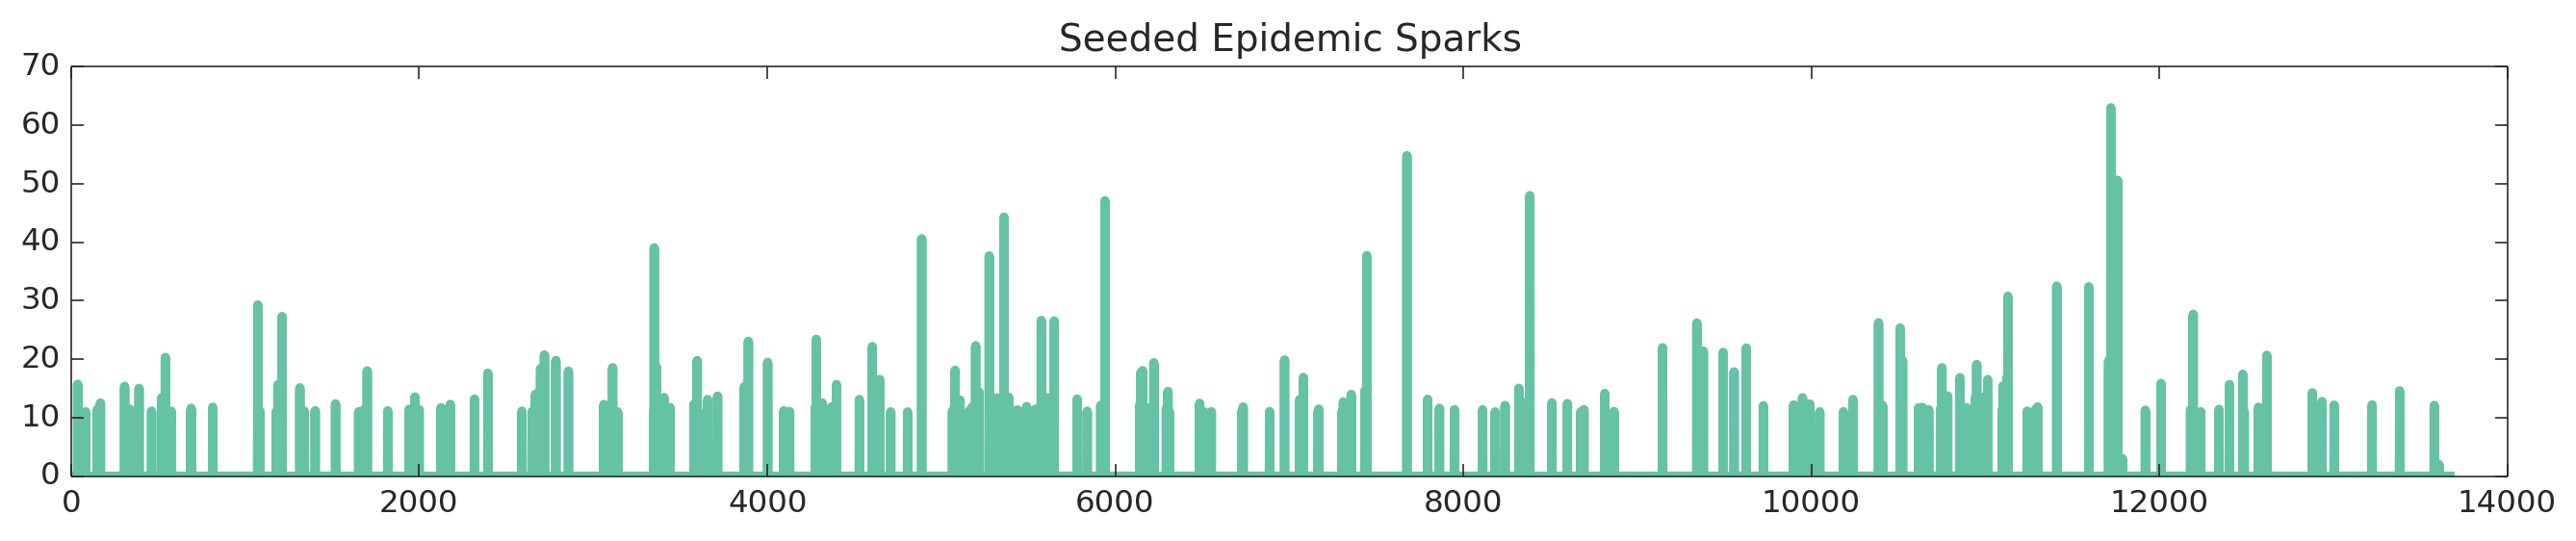
\includegraphics[max size={\textwidth}{\textheight}]{notebook_files/notebook_26_2.png}
    \par
    \end{center}
    
            \end{InvisibleVerbatim}
            
        
    


    % Make sure that atleast 4 lines are below the HR
    \needspace{4\baselineskip}

    
        \vspace{6pt}
        \makebox[0.1\linewidth]{\smaller\hfill\tt\color{nbframe-in-prompt}In\hspace{4pt}{[}{]}:\hspace{4pt}}\\*
        \vspace{-2.65\baselineskip}
        \begin{ColorVerbatim}
            \vspace{-0.7\baselineskip}
            \begin{Verbatim}[commandchars=\\\{\}]
\PY{n}{plt}\PY{o}{.}\PY{n}{plot}\PY{p}{(}\PY{n}{zz}\PY{p}{[}\PY{o}{\PYZhy{}}\PY{n+nb}{len}\PY{p}{(}\PY{n}{C}\PY{p}{)}\PY{p}{:}\PY{p}{]}\PY{p}{)}
\end{Verbatim}

            
                \vspace{-0.2\baselineskip}
            
        \end{ColorVerbatim}
    


    % Make sure that atleast 4 lines are below the HR
    \needspace{4\baselineskip}

    
        \vspace{6pt}
        \makebox[0.1\linewidth]{\smaller\hfill\tt\color{nbframe-in-prompt}In\hspace{4pt}{[}{]}:\hspace{4pt}}\\*
        \vspace{-2.65\baselineskip}
        \begin{ColorVerbatim}
            \vspace{-0.7\baselineskip}
            \begin{Verbatim}[commandchars=\\\{\}]

\end{Verbatim}

            
                \vspace{0.3\baselineskip}
            
        \end{ColorVerbatim}
    


    % Make sure that atleast 4 lines are below the HR
    \needspace{4\baselineskip}

    
        \vspace{6pt}
        \makebox[0.1\linewidth]{\smaller\hfill\tt\color{nbframe-in-prompt}In\hspace{4pt}{[}{]}:\hspace{4pt}}\\*
        \vspace{-2.65\baselineskip}
        \begin{ColorVerbatim}
            \vspace{-0.7\baselineskip}
            \begin{Verbatim}[commandchars=\\\{\}]
\PY{n}{xax} \PY{o}{=} \PY{n}{np}\PY{o}{.}\PY{n}{array}\PY{p}{(}\PY{p}{[}\PY{n}{predSs}\PY{p}{[}\PY{n}{e}\PY{p}{[}\PY{l+m+mi}{0}\PY{p}{]}\PY{p}{]} \PY{k}{for} \PY{n}{e} \PY{o+ow}{in} \PY{n}{epis}\PY{p}{]}\PY{p}{)}\PY{o}{.}\PY{n}{reshape}\PY{p}{(}\PY{n+nb}{len}\PY{p}{(}\PY{n}{actualsizess}\PY{p}{)}\PY{p}{,}\PY{l+m+mi}{1}\PY{p}{)}

\PY{n}{sizelines2} \PY{o}{=} \PY{n}{linear\PYZus{}model}\PY{o}{.}\PY{n}{BayesianRidge}\PY{p}{(}\PY{n}{compute\PYZus{}score}\PY{o}{=}\PY{n+nb+bp}{True}\PY{p}{,} \PY{n}{fit\PYZus{}intercept}\PY{o}{=}\PY{n+nb+bp}{True}\PY{p}{)}
\PY{n}{sizelines3} \PY{o}{=} \PY{n}{linear\PYZus{}model}\PY{o}{.}\PY{n}{BayesianRidge}\PY{p}{(}\PY{n}{compute\PYZus{}score}\PY{o}{=}\PY{n+nb+bp}{True}\PY{p}{,} \PY{n}{fit\PYZus{}intercept}\PY{o}{=}\PY{n+nb+bp}{True}\PY{p}{)}
\PY{n}{sizelines2}\PY{o}{.}\PY{n}{fit}\PY{p}{(}\PY{n}{xax}\PY{p}{,} \PY{n}{actualsizess}\PY{p}{)}
\PY{n}{sizelines3}\PY{o}{.}\PY{n}{fit}\PY{p}{(}\PY{n}{xax}\PY{p}{,} \PY{n}{predictedsizess}\PY{p}{)}

\PY{n}{plt}\PY{o}{.}\PY{n}{scatter}\PY{p}{(}\PY{n}{xax}\PY{p}{,} \PY{n}{actualsizess}\PY{p}{,} \PY{n}{color}\PY{o}{=}\PY{n}{colours}\PY{p}{[}\PY{l+m+mi}{2}\PY{p}{]}\PY{p}{)}
\PY{n}{plt}\PY{o}{.}\PY{n}{scatter}\PY{p}{(}\PY{n}{xax}\PY{p}{,} \PY{n}{predictedsizess}\PY{p}{,} \PY{n}{color}\PY{o}{=}\PY{n}{colours}\PY{p}{[}\PY{l+m+mi}{1}\PY{p}{]}\PY{p}{)}
\PY{n}{plt}\PY{o}{.}\PY{n}{plot}\PY{p}{(}\PY{n}{xax}\PY{p}{,} \PY{n}{sizelines2}\PY{o}{.}\PY{n}{predict}\PY{p}{(}\PY{n}{xax}\PY{p}{)}\PY{p}{,} \PY{n}{linewidth}\PY{o}{=}\PY{l+m+mi}{3}\PY{p}{,} \PY{n}{color}\PY{o}{=}\PY{n}{colours}\PY{p}{[}\PY{l+m+mi}{2}\PY{p}{]}\PY{p}{)}
\PY{n}{plt}\PY{o}{.}\PY{n}{plot}\PY{p}{(}\PY{n}{xax}\PY{p}{,} \PY{n}{sizelines3}\PY{o}{.}\PY{n}{predict}\PY{p}{(}\PY{n}{xax}\PY{p}{)}\PY{p}{,} \PY{n}{linewidth}\PY{o}{=}\PY{l+m+mi}{3}\PY{p}{,} \PY{n}{color}\PY{o}{=}\PY{n}{colours}\PY{p}{[}\PY{l+m+mi}{1}\PY{p}{]}\PY{p}{)}

\PY{n}{legend}\PY{p}{(}\PY{p}{[}\PY{l+s}{r\PYZdq{}}\PY{l+s}{Actual Sizes, \PYZdl{}R\PYZca{}2\PYZdl{} = }\PY{l+s}{\PYZdq{}} \PY{o}{+} \PY{n+nb}{str}\PY{p}{(}\PY{n}{sizelines2}\PY{o}{.}\PY{n}{score}\PY{p}{(}\PY{n}{xax}\PY{p}{,} \PY{n}{actualsizess}\PY{p}{)}\PY{p}{)}\PY{p}{,} \PY{l+s}{r\PYZdq{}}\PY{l+s}{Predicted Sizes, \PYZdl{}R\PYZca{}2\PYZdl{} = }\PY{l+s}{\PYZdq{}} \PY{o}{+} \PY{n+nb}{str}\PY{p}{(}\PY{n}{sizelines3}\PY{o}{.}\PY{n}{score}\PY{p}{(}\PY{n}{xax}\PY{p}{,} \PY{n}{predictedsizess}\PY{p}{)}\PY{p}{)}\PY{p}{]}\PY{p}{)}
\PY{n}{xlabel}\PY{p}{(}\PY{l+s}{r\PYZdq{}}\PY{l+s}{Initial Susceptibles, \PYZdl{}S\PYZus{}0\PYZdl{}}\PY{l+s}{\PYZdq{}}\PY{p}{)}
\PY{n}{ylabel}\PY{p}{(}\PY{l+s}{\PYZdq{}}\PY{l+s}{Size of Epidemic}\PY{l+s}{\PYZdq{}}\PY{p}{)}
\PY{n}{title}\PY{p}{(}\PY{l+s}{\PYZdq{}}\PY{l+s}{Epidemic Sizes vs Initial Susceptible Number}\PY{l+s}{\PYZdq{}}\PY{p}{)}
\end{Verbatim}

            
                \vspace{-0.2\baselineskip}
            
        \end{ColorVerbatim}
    


    % Make sure that atleast 4 lines are below the HR
    \needspace{4\baselineskip}

    
        \vspace{6pt}
        \makebox[0.1\linewidth]{\smaller\hfill\tt\color{nbframe-in-prompt}In\hspace{4pt}{[}{]}:\hspace{4pt}}\\*
        \vspace{-2.65\baselineskip}
        \begin{ColorVerbatim}
            \vspace{-0.7\baselineskip}
            \begin{Verbatim}[commandchars=\\\{\}]

\end{Verbatim}

            
                \vspace{0.3\baselineskip}
            
        \end{ColorVerbatim}
    


    % Make sure that atleast 4 lines are below the HR
    \needspace{4\baselineskip}

    
        \vspace{6pt}
        \makebox[0.1\linewidth]{\smaller\hfill\tt\color{nbframe-in-prompt}In\hspace{4pt}{[}{]}:\hspace{4pt}}\\*
        \vspace{-2.65\baselineskip}
        \begin{ColorVerbatim}
            \vspace{-0.7\baselineskip}
            \begin{Verbatim}[commandchars=\\\{\}]
\PY{c}{\PYZsh{} OLD CODE}

\PY{l+s+sd}{\PYZdq{}\PYZdq{}\PYZdq{}    }
\PY{l+s+sd}{    }
\PY{l+s+sd}{\PYZsh{} Run some R nastiness to obtain the most likely Sbar as well as periodicity and alpha}
\PY{l+s+sd}{\PYZsh{} This is currently being replaced by some Python magic}



\PY{l+s+sd}{\PYZsh{} Write a dataframe to file}
\PY{l+s+sd}{d = \PYZob{}\PYZcb{}}
\PY{l+s+sd}{d[\PYZdq{}logIt\PYZdq{}] = np.log(rho[z[1:]] * C[z[1:]])}
\PY{l+s+sd}{d[\PYZdq{}Z\PYZdq{}] = Z[z[:\PYZhy{}1]]}
\PY{l+s+sd}{d[\PYZdq{}logIt1\PYZdq{}] = np.log(rho[z[:\PYZhy{}1]] * C[z[:\PYZhy{}1]])}
\PY{l+s+sd}{d[\PYZdq{}r\PYZdq{}] = np.tile(range(int(periodicity)), 100)[z[1:]]}

\PY{l+s+sd}{df = DataFrame(d)}
\PY{l+s+sd}{df.to\PYZus{}csv(\PYZdq{}dataframe.csv\PYZdq{})}




\PY{l+s+sd}{\PYZsh{} Call R, load dataframe, run a generalised linear model fit}
\PY{l+s+sd}{ro.r(\PYZsq{}d \PYZlt{}\PYZhy{} read.csv(\PYZdq{}dataframe.csv\PYZdq{})\PYZsq{})}
\PY{l+s+sd}{ro.r(\PYZsq{}S \PYZlt{}\PYZhy{}seq(abs(min(d\PYZdl{}Z))+1, abs(min(d\PYZdl{}Z))*13, by=500)\PYZsq{})}
\PY{l+s+sd}{ro.r(\PYZsq{}l \PYZlt{}\PYZhy{} rep(NA, length(S))\PYZsq{})}
\PY{l+s+sd}{ro.r(\PYZsq{}d\PYZdl{}r\PYZlt{}\PYZhy{}as.factor(d\PYZdl{}r)\PYZsq{})}

\PY{l+s+sd}{ro.r(\PYZdq{}for(i in 1:length(S)) \PYZob{} \PYZbs{}}
\PY{l+s+sd}{                                 logS \PYZlt{}\PYZhy{} log(S[i] + d\PYZdl{}Z);     \PYZbs{}}
\PY{l+s+sd}{                                 m \PYZlt{}\PYZhy{} glm( d\PYZdl{}logIt \PYZti{} \PYZhy{}1 + d\PYZdl{}r + d\PYZdl{}logIt1 + offset(logS) );     \PYZbs{}}
\PY{l+s+sd}{                                 l[i] = m\PYZdl{}deviance     \PYZbs{}}
\PY{l+s+sd}{                            \PYZcb{}\PYZdq{})}
\PY{l+s+sd}{ro.r(\PYZdq{}m2 \PYZlt{}\PYZhy{} glm( d\PYZdl{}logIt \PYZti{} \PYZhy{}1 + d\PYZdl{}r + d\PYZdl{}logIt1 + offset(log(S[l == min(l)] + d\PYZdl{}Z)) )\PYZdq{})}
\PY{l+s+sd}{ro.r(\PYZdq{}ci \PYZlt{}\PYZhy{} confint(m2)\PYZdq{})   }

\PY{l+s+sd}{    }
\PY{l+s+sd}{    }

\PY{l+s+sd}{\PYZsh{} Extract variables of interest from R}
\PY{l+s+sd}{L = \PYZhy{}np.array(ro.r[\PYZdq{}l\PYZdq{}])}
\PY{l+s+sd}{coefs = np.array(ro.r(\PYZdq{}coef(m2)\PYZdq{}))}
\PY{l+s+sd}{Svals = np.array(ro.r[\PYZdq{}S\PYZdq{}])}
\PY{l+s+sd}{Sbar = Svals[np.argmax(L)]}
\PY{l+s+sd}{r = np.exp(coefs[:periodicity])}
\PY{l+s+sd}{alphaSbar = coefs[periodicity]}
\PY{l+s+sd}{ci = np.exp(ro.r[\PYZdq{}ci\PYZdq{}])}




\PY{l+s+sd}{\PYZsh{} Plot}
\PY{l+s+sd}{subplot(121)}
\PY{l+s+sd}{plt.axvline(x=Sbar, color=colours[1], linewidth=2)}
\PY{l+s+sd}{plt.axvline(x=1/zeta, color=colours[2], linewidth=2)}
\PY{l+s+sd}{plt.plot(Svals, np.exp(L), linewidth=3)}
\PY{l+s+sd}{title(\PYZdq{}Likelihood landscape vs Sbar\PYZdq{})}
\PY{l+s+sd}{legend([r\PYZdq{}Profile Likelihood \PYZdl{}\PYZbs{}bar\PYZob{}S\PYZcb{}\PYZdl{} = \PYZdq{} + str(int(Sbar)), r\PYZdq{}Taylor Expansion \PYZdl{}\PYZbs{}bar\PYZob{}S\PYZcb{}\PYZdl{} = \PYZdq{} + str(int(1/zeta))], loc=4)}

\PY{l+s+sd}{subplot(122)}
\PY{l+s+sd}{\PYZsh{}plt.plot(rstar, linewidth=2)}
\PY{l+s+sd}{plt.plot(r, linewidth=3)}
\PY{l+s+sd}{plt.fill\PYZus{}between(range(periodicity), ci[:\PYZhy{}1, 0], ci[:\PYZhy{}1, 1], color=colours[0], alpha=0.3)}
\PY{l+s+sd}{plt.plot(np.roll(rstar * zeta, 1), linewidth=3)}
\PY{l+s+sd}{xlim([0, periodicity])}
\PY{l+s+sd}{title(\PYZdq{}Periodicity\PYZdq{})}
\PY{l+s+sd}{legend([\PYZdq{}Using Full Equation\PYZdq{}, \PYZdq{}Using Taylor Expansion\PYZdq{}])}
\PY{l+s+sd}{\PYZdq{}\PYZdq{}\PYZdq{}}
\end{Verbatim}

            
                \vspace{-0.2\baselineskip}
            
        \end{ColorVerbatim}
    


    % Make sure that atleast 4 lines are below the HR
    \needspace{4\baselineskip}

    
        \vspace{6pt}
        \makebox[0.1\linewidth]{\smaller\hfill\tt\color{nbframe-in-prompt}In\hspace{4pt}{[}{]}:\hspace{4pt}}\\*
        \vspace{-2.65\baselineskip}
        \begin{ColorVerbatim}
            \vspace{-0.7\baselineskip}
            \begin{Verbatim}[commandchars=\\\{\}]
\PY{c}{\PYZsh{} What about inferring using pure MCMC ?}
\PY{c}{\PYZsh{} Let\PYZsq{}s infer from Equation 12}

\PY{c}{\PYZsh{}\PYZsh{} CURRENTLY COMMENTED OUT}

\PY{l+s+sd}{\PYZdq{}\PYZdq{}\PYZdq{}}
\PY{l+s+sd}{with pymc.Model() as model :}
\PY{l+s+sd}{    }
\PY{l+s+sd}{    \PYZsh{} The prior on Sbar can be informed from earlier calculation}
\PY{l+s+sd}{    SbarMC = pymc.Normal(\PYZdq{}SbarMC\PYZdq{}, Sbar, 1e\PYZhy{}10)}
\PY{l+s+sd}{    }
\PY{l+s+sd}{    \PYZsh{} Alpha}
\PY{l+s+sd}{    alphaMC = pymc.Beta(\PYZdq{}alphaMC\PYZdq{}, 2., 1.)}
\PY{l+s+sd}{    }
\PY{l+s+sd}{    \PYZsh{} r}
\PY{l+s+sd}{    rMC = pymc.Normal(\PYZdq{}rMC\PYZdq{}, \PYZhy{}12., 0.3, shape=periodicity)}
\PY{l+s+sd}{    }
\PY{l+s+sd}{    EIMC = np.tile(rMC, 2*len(C)/periodicity)[:len(rho[:\PYZhy{}1])] + alphaMC * np.log(rho*C)[:\PYZhy{}1] + np.log(Sbar + Z[:\PYZhy{}1])}
\PY{l+s+sd}{    }
\PY{l+s+sd}{    }
\PY{l+s+sd}{    \PYZsh{} Expected cases}
\PY{l+s+sd}{    @pymc.deterministic}
\PY{l+s+sd}{    def EIMC(r = rMC, a = alphaMC, Sbar = SbarMC, It = np.log(rho * C), Z = Z) :}
\PY{l+s+sd}{        out = np.zeros\PYZus{}like(It)}
\PY{l+s+sd}{        out[0] = It[0]}
\PY{l+s+sd}{        for i in range(1, len(It)) :}
\PY{l+s+sd}{            out[i] = r[i \PYZpc{} periodicity] + a * It[i\PYZhy{}1] + np.log(Sbar + Z[i\PYZhy{}1])}
\PY{l+s+sd}{        return out}
\PY{l+s+sd}{    }
\PY{l+s+sd}{    }
\PY{l+s+sd}{    \PYZsh{} Observed cases}
\PY{l+s+sd}{    IMC = pymc.Normal(\PYZdq{}IMC\PYZdq{}, EIMC, 1./np.var(np.log(rho*C)), observed=True, value=np.log(rho * C))}
\PY{l+s+sd}{    }
\PY{l+s+sd}{    start = find\PYZus{}MAP() \PYZsh{} Find starting value by optimization}
\PY{l+s+sd}{    step = NUTS(state=start) \PYZsh{} Instantiate MCMC sampling algorithm}
\PY{l+s+sd}{    trace = sample(2000, step, start=start, progressbar=False) \PYZsh{} draw 2000 posterior }
\PY{l+s+sd}{    }
\PY{l+s+sd}{    }
\PY{l+s+sd}{    \PYZsh{}model = pymc.Model((SbarMC, alphaMC, rMC, EIMC, IMC))}
\PY{l+s+sd}{    \PYZsh{}mcmc = pymc.MCMC(model)}
\PY{l+s+sd}{    \PYZsh{}mcmc.sample(200000)}
\PY{l+s+sd}{\PYZdq{}\PYZdq{}\PYZdq{}}
\end{Verbatim}

            
                \vspace{-0.2\baselineskip}
            
        \end{ColorVerbatim}
    


    % Make sure that atleast 4 lines are below the HR
    \needspace{4\baselineskip}

    
        \vspace{6pt}
        \makebox[0.1\linewidth]{\smaller\hfill\tt\color{nbframe-in-prompt}In\hspace{4pt}{[}{]}:\hspace{4pt}}\\*
        \vspace{-2.65\baselineskip}
        \begin{ColorVerbatim}
            \vspace{-0.7\baselineskip}
            \begin{Verbatim}[commandchars=\\\{\}]

\end{Verbatim}

            
                \vspace{0.3\baselineskip}
            
        \end{ColorVerbatim}
    


    % Make sure that atleast 4 lines are below the HR
    \needspace{4\baselineskip}

    
        \vspace{6pt}
        \makebox[0.1\linewidth]{\smaller\hfill\tt\color{nbframe-in-prompt}In\hspace{4pt}{[}{]}:\hspace{4pt}}\\*
        \vspace{-2.65\baselineskip}
        \begin{ColorVerbatim}
            \vspace{-0.7\baselineskip}
            \begin{Verbatim}[commandchars=\\\{\}]

\end{Verbatim}

            
                \vspace{0.3\baselineskip}
            
        \end{ColorVerbatim}
    

        

        \renewcommand{\indexname}{Index}
        \printindex

    % End of document
    \end{document}


